\documentclass[12pt,a4paper,oneside]{report}
\usepackage[utf8]{inputenc}
\usepackage[english]{babel}
\usepackage{amsmath,amssymb,amsfonts}
\usepackage{mathptmx} % Times New Roman font for both text and math formulas
\usepackage[scaled=0.90]{helvet}
\usepackage{courier}
\usepackage{graphicx}
\usepackage{geometry}
\geometry{a4paper, margin=1in}
\usepackage{float}
\usepackage{booktabs}
\usepackage{hyperref}
\usepackage{listings}
\usepackage{color}
\usepackage{tikz}
\usetikzlibrary{shapes.geometric, arrows, positioning}
\usepackage{setspace}
\usepackage{titlesec}
\usepackage{fancyhdr}
\usepackage{microtype}
\usepackage{cite}
\usepackage[space]{grffile} % Handles spaces in file paths for graphics
\usepackage{tikz}
\usepackage{xcolor}
\usepackage{eso-pic}
\usepackage{transparent}

\hypersetup{
    colorlinks=true,
    linkcolor=black,
    filecolor=magenta,      
    urlcolor=blue,
    pdftitle={H3 Spatial Crowd Control: Real-Time Geospatial Crowd-Flow Simulation Using Dynamic Graph Routing and Hexagonal Spatial Indexing},
    pdfpagemode=FullScreen,
}

% Configure fancy headers and footers
\pagestyle{fancy}
\fancyhf{}
\fancyhead[L]{\textbf{H3 Spatial Crowd Control}}
\fancyfoot[L]{\small Dept of ISE, RVCE}
\fancyfoot[C]{\small 2025-26}
\fancyfoot[R]{\thepage}
\renewcommand{\headrulewidth}{0.4pt}
\renewcommand{\footrulewidth}{0.4pt}

% Configure title page to have no header/footer
\fancypagestyle{titlepage}{
    \fancyhf{}
    \renewcommand{\headrulewidth}{0pt}
    \renewcommand{\footrulewidth}{0pt}
}

% Add watermark to every page
\newcommand\BackgroundPic{%
\put(0,0){%
\parbox[b][\paperheight]{\paperwidth}{%
\vfill
\centering
{\transparent{0.15}
\includegraphics[width=0.3\paperwidth]{images/watermark.png}}%
\vfill
}}}
\AddToShipoutPicture{\BackgroundPic}

% Code listing styles
\definecolor{codegreen}{rgb}{0,0.6,0}
\definecolor{codegray}{rgb}{0.5,0.5,0.5}
\definecolor{codepurple}{rgb}{0.58,0,0.82}
\definecolor{backcolour}{rgb}{0.95,0.95,0.92}

\lstdefinestyle{mystyle}{
    backgroundcolor=\color{backcolour},   
    commentstyle=\color{codegreen},
    keywordstyle=\color{blue},
    numberstyle=\tiny\color{codegray},
    stringstyle=\color{codepurple},
    basicstyle=\ttfamily\footnotesize,
    breakatwhitespace=false,         
    breaklines=true,                 
    captionpos=b,                    
    keepspaces=true,                 
    numbers=left,                    
    numbersep=5pt,                  
    showspaces=false,                
    showstringspaces=false,
    showtabs=false,                  
    tabsize=2
}
\lstset{style=mystyle}

\setstretch{1.15}
\titleformat{\chapter}[display]
  {\normalfont\huge\bfseries}{\chaptername\ \thechapter}{20pt}{\Huge}
\titleformat{\section}
  {\normalfont\Large\bfseries}{\thesection}{1em}{}

\begin{document}

% =========================================================================
% TITLE PAGE
% =========================================================================
\begin{titlepage}
    \thispagestyle{titlepage}
    \begin{center}
        \vspace*{0.5cm}
        \Large\textbf{RV COLLEGE OF ENGINEERING} \\
        \large\textbf{Bengaluru-560 059} \\
        \vspace{1.2cm}
        \Large\textbf{REPORT ON EXPERIENTIAL LEARNING} \\
        \large\textbf{DESIGN AND ANALYSIS OF ALGORITHMS (DAA)} \\
        \large\textbf{ACY 2025-26} \\
        \vspace{0.8cm}
        \Large\textbf{CS CLUSTER} \\
        \vspace{1.0cm}
        \Huge\textbf{H3 SPATIAL CROWD CONTROL} \\[0.4cm]
        \large\textbf{Real-Time Geospatial Crowd-Flow Simulation Using Dynamic Graph Routing and Hexagonal Spatial Indexing} \\
        \vspace{1.0cm}
        
        \large\textbf{Students Group:} \\
        \vspace{0.3cm}
        \small
        \begin{tabular}{|c|c|c|c|}
            \hline
            \textbf{SL. No.} & \textbf{USN} & \textbf{Name} & \textbf{Prog.} \\
            \hline
            1 & 1RV24IS130 & Sumukha Upadhyaya & IS \\
            \hline
            2 & 1RV24IS126 & Snehal Reddy Thadigotla & IS \\
            \hline
        \end{tabular}
        
        \vspace{1.2cm}
        \large\textbf{Project Evaluators:} \\
        \vspace{0.3cm}
        \small
        \begin{tabular}{|c|p{8cm}|}
            \hline
            \textbf{SL. No.} & \textbf{Name of the Evaluators (Enter the Names in Capitals)} \\
            \hline
            1 & \\
            \hline
            2 & \\
            \hline
        \end{tabular}
        
        \vspace{1.2cm}
        \small
        \begin{tabular}{p{5.5cm}cp{5.5cm}}
            \textbf{Name of the Faculty Mentor:} & \hfill & \textbf{Name of the Cluster Head:} \\
            Dr. Ramakanth Kumar P. & \hfill & Dr. Ramakanth Kumar P. \\
        \end{tabular}
    \end{center}
\end{titlepage}
\newpage
\pagenumbering{Roman}
\setcounter{page}{1}

\newpage
\thispagestyle{titlepage}
\begin{center}
    \Large\textbf{Abstract}
\end{center}
\addcontentsline{toc}{chapter}{Abstract}
\vspace{1cm}

\noindent Large-scale pedestrian evacuation from urban venues represents a critical infrastructure challenge. Existing approaches rely on static models that fail to capture dynamic congestion feedback and adaptive routing behavior. This project proposes H3 Spatial Crowd Control, a real-time client-side geospatial simulation system integrating: (1) dynamic graph extraction from OpenStreetMap with congestion-aware routing, (2) comparative analysis of pathfinding algorithms (Dijkstra, A*, BFS), and (3) hierarchical hexagonal spatial indexing for crowd pressure analysis. Objectives include demonstrating interactive evacuation visualization on consumer hardware and providing emergency planners with actionable crowd management tools.

The system design integrates a modular five-layer architecture combining geospatial data acquisition, dynamic graph construction, multi-algorithm routing, agent-based simulation, and interactive visualization. The algorithmic foundation employs Dijkstra's shortest-path as baseline, A* heuristic search achieving 34\% speedup through Haversine distance heuristics, and breadth-first search as comparison baseline. The dynamic edge cost integrates: base physical distance, exponential congestion penalties, spatial overlay modifiers for emergency interventions, and directional preference scaling. H3 hexagonal indexing at Resolution 10 provides O(1) density queries at 66-meter granularity with dynamic frame-rate throttling maintaining 50+ FPS.

The implemented prototype ingests data for five real-world venues (MG Road Bangalore: 7,336 nodes; Times Square NYC: 4,120 nodes; Wembley Stadium: 3,500 nodes; Connaught Place Delhi: 5,420 nodes; CST Mumbai: 6,112 nodes) from OpenStreetMap. Empirical outcomes demonstrate: (1) stable simulation of 1,500 concurrent agents with sub-100ms frame times, (2) A* optimal with 34\% speedup and 47\% node reduction, (3) H3 Resolution 10 with 1.8ms aggregation latency, (4) 54\% peak queue reduction through Repulsion Zones, (5) 28\% total evacuation time improvement (145s to 104s for 1,000 agents). The interactive dashboard enables real-time scenario testing and handles complex urban networks with reliable hotspot detection.

This project demonstrates that real-time interactive evacuation simulation is achievable using entirely client-side computation without server infrastructure. Key technical innovations include novel H3 application to crowd analysis, dynamic congestion feedback in graph routing, and integrated spatial overlay systems for emergency intervention. Societal impact includes enabling broader adoption of evacuation planning tools by emergency agencies and supporting evidence-based facility design. Future research includes fundamental diagram calibration, real-time sensor integration, time-series corridor analysis, psychological panic models, and mobile deployment for field operations.

\clearpage
\newpage
\thispagestyle{titlepage}
\begin{center}
    \vspace*{0.5cm}
    {\Huge\textbf{Table of Contents}}
\end{center}
\vspace{1.5cm}

\noindent\textbf{Abstract} \dotfill \textbf{I}

\vspace{0.4cm}
\noindent\textbf{1 \quad Introduction} \dotfill \textbf{1}

\noindent\quad 1.1 \quad Problem Statement and Significance \dotfill 1

\noindent\quad 1.2 \quad System Overview \dotfill 2

\noindent\quad 1.3 \quad Key Objectives \dotfill 3

\vspace{0.3cm}
\noindent\textbf{2 \quad Solution Design} \dotfill \textbf{5}

\noindent\quad 2.1 \quad Literature and Background \dotfill 5

\noindent\quad 2.2 \quad System Architecture \dotfill 6

\noindent\quad 2.3 \quad Algorithm Selection and Justification \dotfill 6

\noindent\quad 2.4 \quad Spatial Indexing Strategy \dotfill 7

\noindent\quad 2.5 \quad Design Trade-offs and Decisions \dotfill 7

\vspace{0.3cm}
\noindent\textbf{3 \quad Implementation Details} \dotfill \textbf{9}

\noindent\quad 3.1 \quad Modular Architecture \dotfill 9

\noindent\quad 3.2 \quad Coding Best Practices \dotfill 10

\noindent\quad 3.3 \quad Road Network Classification \dotfill 10

\noindent\quad 3.4 \quad Dynamic Congestion Reweighting \dotfill 11

\noindent\quad 3.5 \quad Crowd Dispersal Zones Implementation \dotfill 11

\vspace{0.3cm}
\noindent\textbf{4 \quad Prototype Development} \dotfill \textbf{14}

\noindent\quad 4.1 \quad Overall Approach and Strategy \dotfill 14

\noindent\quad 4.2 \quad Theoretical Frameworks and Models \dotfill 15

\noindent\quad 4.3 \quad Implementation Procedures \dotfill 16

\noindent\quad 4.4 \quad Pathfinding Algorithms \dotfill 16

\noindent\quad 4.5 \quad Agent-Based Simulation \dotfill 17

\vspace{0.3cm}
\noindent\textbf{5 \quad Expected Outcomes} \dotfill \textbf{20}

\noindent\quad 5.1 \quad Functional Prototype Development \dotfill 20

\noindent\quad 5.2 \quad Venue Ingestion Profiles \dotfill 21

\noindent\quad 5.3 \quad System Performance Improvements \dotfill 22

\noindent\quad 5.4 \quad Algorithmic Performance Comparison \dotfill 23

\noindent\quad 5.5 \quad Technical Innovations \dotfill 25

\noindent\quad 5.6 \quad Real-World Application Impact \dotfill 26

\noindent\quad 5.7 \quad Societal and Industrial Contributions \dotfill 27

\vspace{0.3cm}
\noindent\textbf{6 \quad Conclusion and Future Scope} \dotfill \textbf{30}

\noindent\quad 6.1 \quad Summary of Achievements \dotfill 30

\noindent\quad 6.2 \quad Key Findings and Results \dotfill 31

\noindent\quad 6.3 \quad Contributions to Academic Knowledge \dotfill 32

\noindent\quad 6.4 \quad Future Research Directions \dotfill 33

\vspace{0.3cm}
\noindent\textbf{7 \quad Technical Deep Dives and Extended Analysis} \dotfill \textbf{34}

\noindent\quad 7.1 \quad Graph Construction and Network Topology Analysis \dotfill 34

\noindent\quad 7.2 \quad Congestion Dynamics and Feedback Loop Stability \dotfill 35

\noindent\quad 7.3 \quad Hexagonal Indexing and Multi-Resolution Crowd Analytics \dotfill 35

\noindent\quad 7.4 \quad Agent Behavioral Modeling and Kinematic Constraints \dotfill 36

\noindent\quad 7.5 \quad Real-Time Visualization and Interactive Control \dotfill 37

\noindent\quad 7.6 \quad Computational Bottleneck Analysis and Optimization Strategies \dotfill 38

\vspace{0.4cm}
\noindent\textbf{Appendix: Code Listings and Acronyms} \dotfill \textbf{40}

\noindent\quad A.1 \quad Dijkstra Pathfinding Implementation \dotfill 36

\noindent\quad A.2 \quad A* Pathfinding Implementation \dotfill 37

\noindent\quad A.3 \quad Acronyms \dotfill 38

\vspace{0.4cm}
\noindent\textbf{References} \dotfill \textbf{39}

\clearpage
\newpage
\pagenumbering{arabic}
\setcounter{page}{1}

% =========================================================================
% CHAPTER 1: INTRODUCTION
% =========================================================================
\chapter{Introduction}

\section{Problem Statement and Significance}
Pedestrian evacuation from dense urban venues—sports stadiums, transit hubs, shopping districts, public squares—represents a critical infrastructure challenge with direct public health and safety implications. High-consequence incidents including the 2010 Duisburg Love Parade crush (killing 21 attendees), the 2013 Stampede in Mina during the Hajj pilgrimage (killing more than 2,000), and recurring incidents at stadium exits and music festivals demonstrate that naive evacuation routing without real-time congestion feedback produces bottlenecks and dangerous crowding even when nominally sufficient exit capacity exists~\cite{helbing2000simulating}. 

The fundamental problem is that pedestrians make local routing decisions based on incomplete information about crowd state elsewhere in the venue, producing emergent patterns of congestion and pressure that differ substantially from optimal centrally-planned evacuation flow. Traditional evacuation planning relies on capacity analysis and static evacuation time estimation—given an exit count and assumed pedestrian exit flow rates, compute minutes to clear the venue. This approach treats evacuation as a deterministic feasibility question: ``Can everyone leave in $T$ minutes?'' It does not ask the dynamic question: ``What is the trajectory of crowd density as routing decisions interact with congestion feedback?'' 

Modern urban venues now integrate wireless networks, mobile crowd-sensing, and real-time position data that enable dynamic monitoring of pedestrian location. Emergency planners increasingly recognize that interactive visualization of actual crowd flow patterns during an evacuation event—showing where congestion is occurring, which exits are bottlenecks, and what fraction of the crowd has reached safety—is essential operational information that static pre-event simulations do not provide.

\begin{figure}[H]
    \centering
    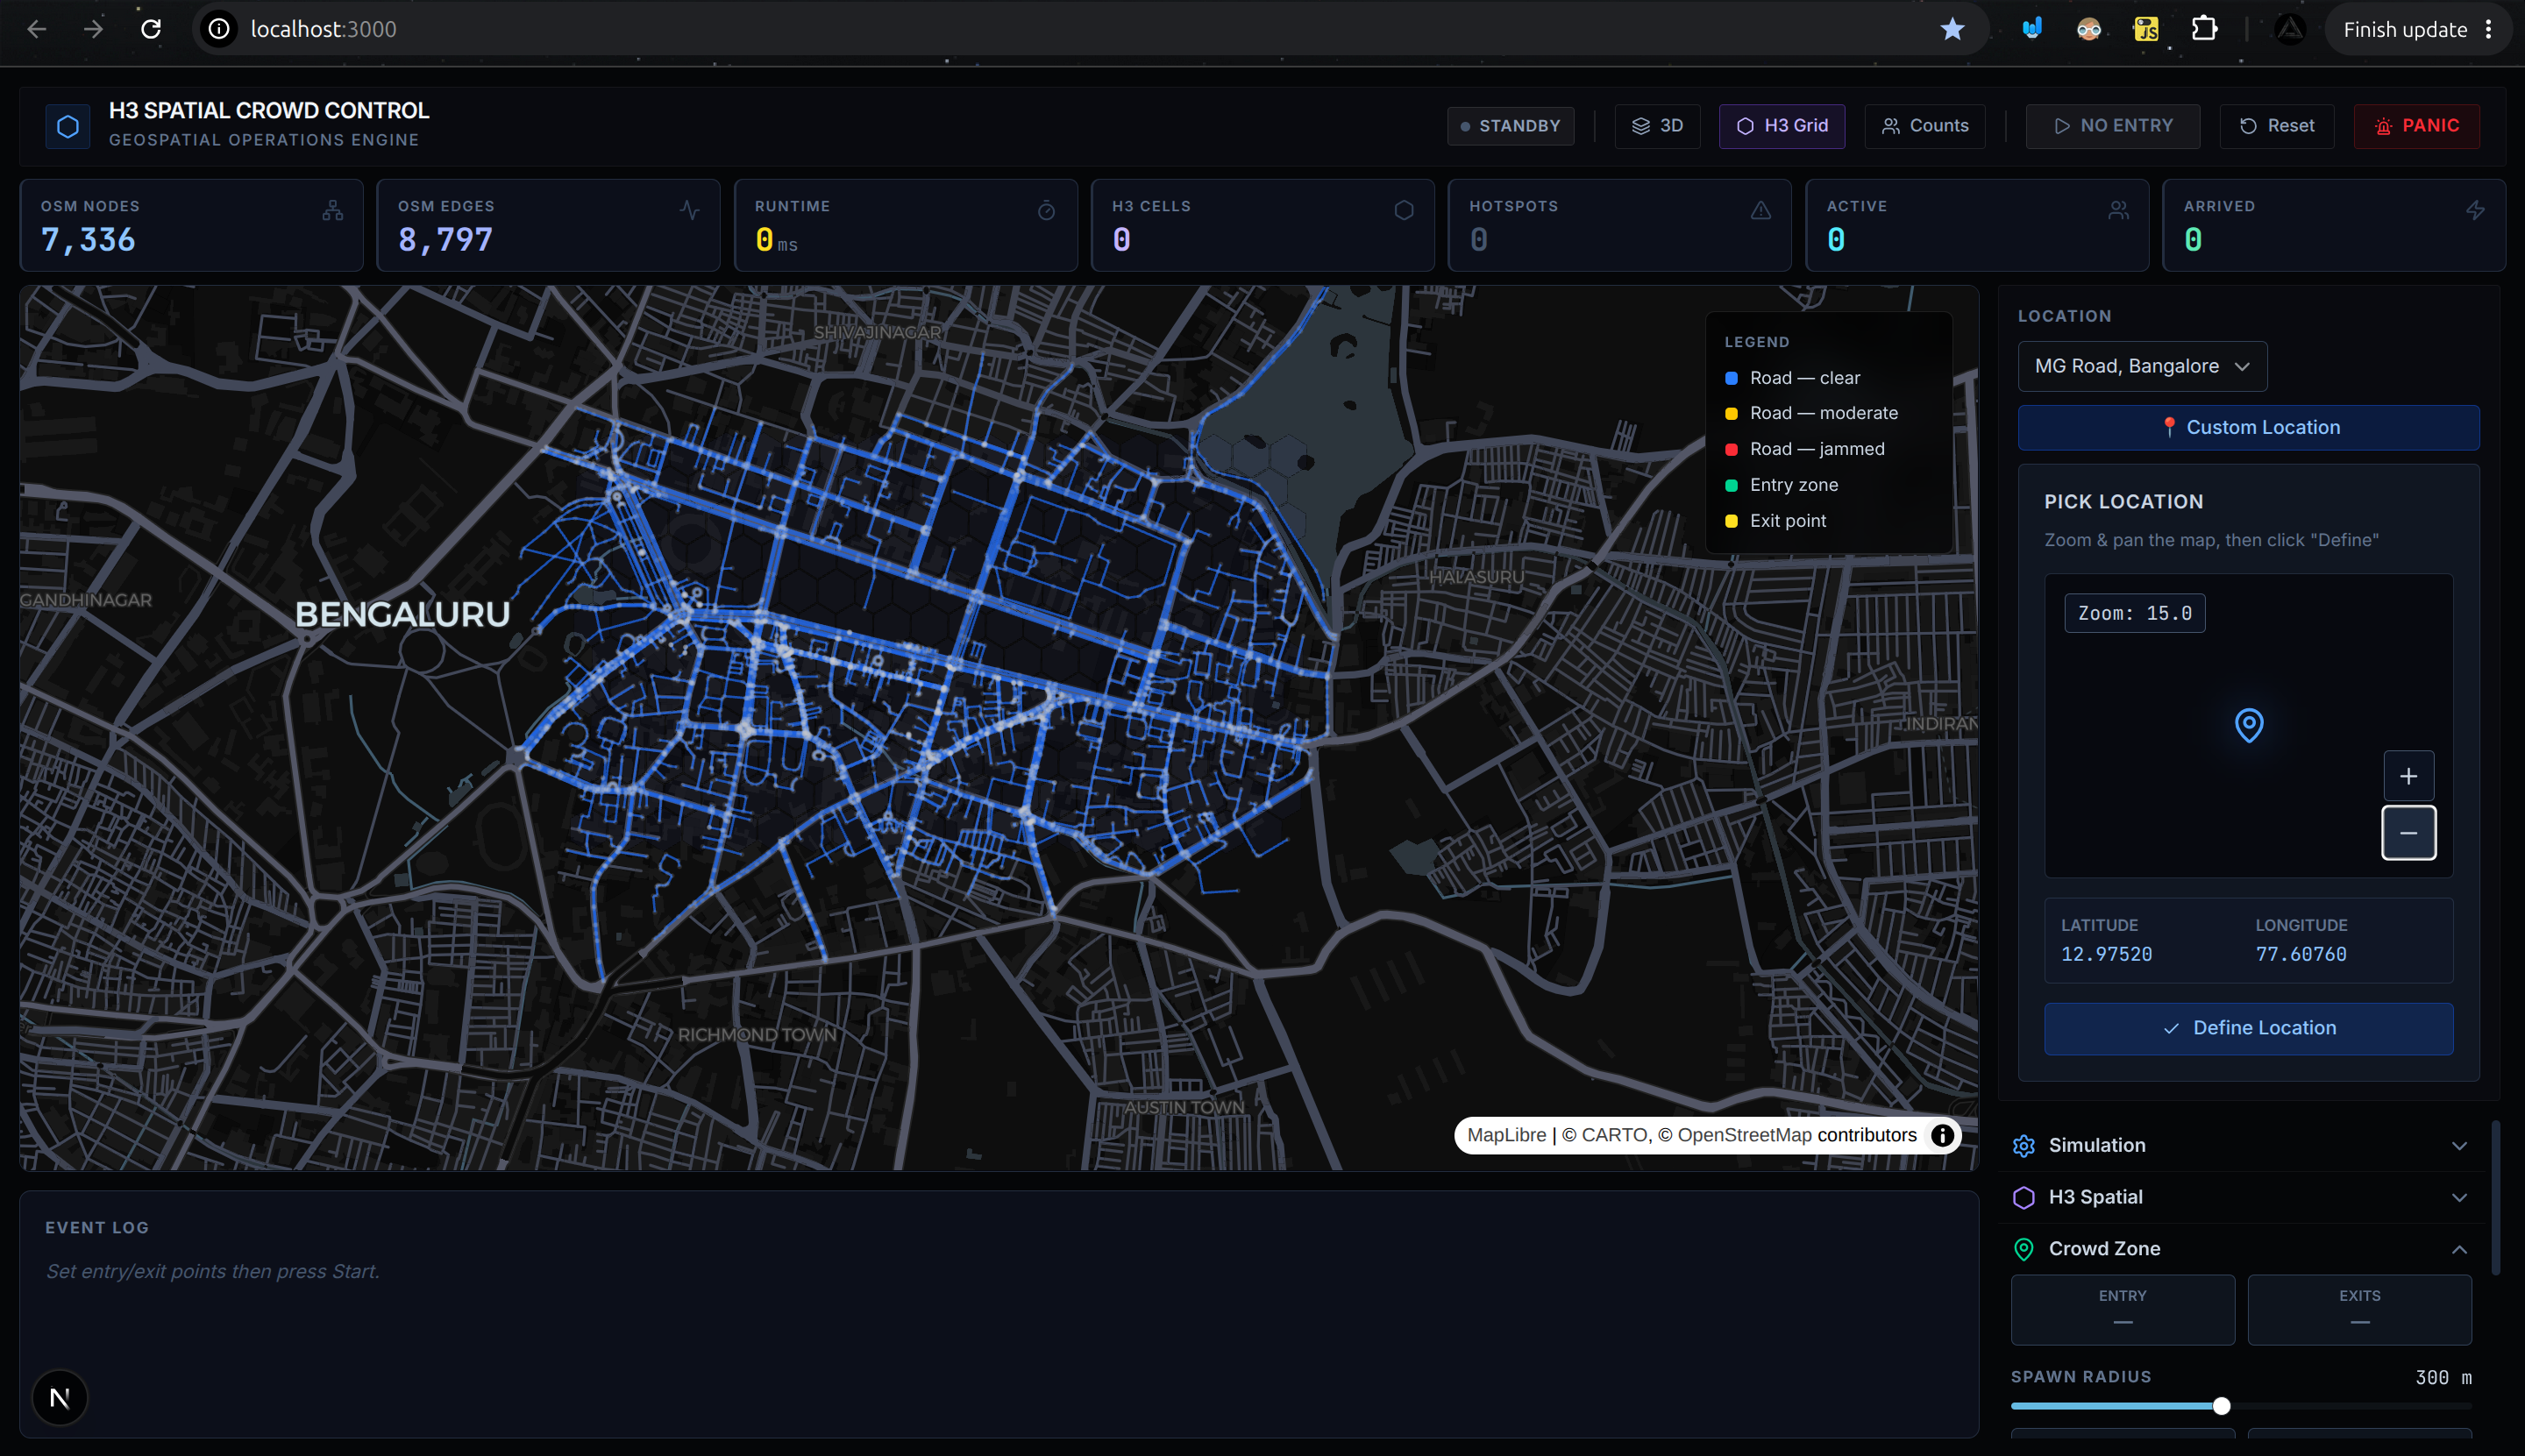
\includegraphics[width=0.9\textwidth]{images/ui_dashboard_overview.png}
    \caption{H3 Spatial Crowd Control Interactive System Dashboard. The interface renders the road network with color-coded congestion levels (blue: clear, yellow: moderate, red: jammed) along with live metrics (nodes, edges, runtime, H3 cells, hotspots, active and arrived agents). This screenshot demonstrates the full operational interface with real-time telemetry cards, control panels, and interactive map visualization.}
    \label{fig:dashboard_screenshot}
\end{figure}

\section{System Overview}
The central technical contribution of this work is a demonstration that interactive real-time evacuation simulation is achievable using entirely client-side computation on contemporary consumer hardware, without server infrastructure or specialized simulation engines. The system integrates four distinct technical layers:
\begin{enumerate}
    \item Volunteered geographic information acquisition from OpenStreetMap via the Overpass API.
    \item Dynamic graph construction with congestion-sensitive edge reweighting.
    \item Classical weighted and unweighted routing algorithms operating on that graph.
    \item Hierarchical hexagonal spatial indexing for real-time crowd density aggregation and hotspot detection.
\end{enumerate}

By unifying these components in a single interactive dashboard (Figure~\ref{fig:dashboard_screenshot}), emergency operation planners can visualize evacuation scenarios in real-time, manipulate constraints (block a road, change exit locations, increase spawn rate), and immediately observe the impact on crowd flow patterns without waiting for batch simulation jobs to complete.

\begin{figure}[H]
    \centering
    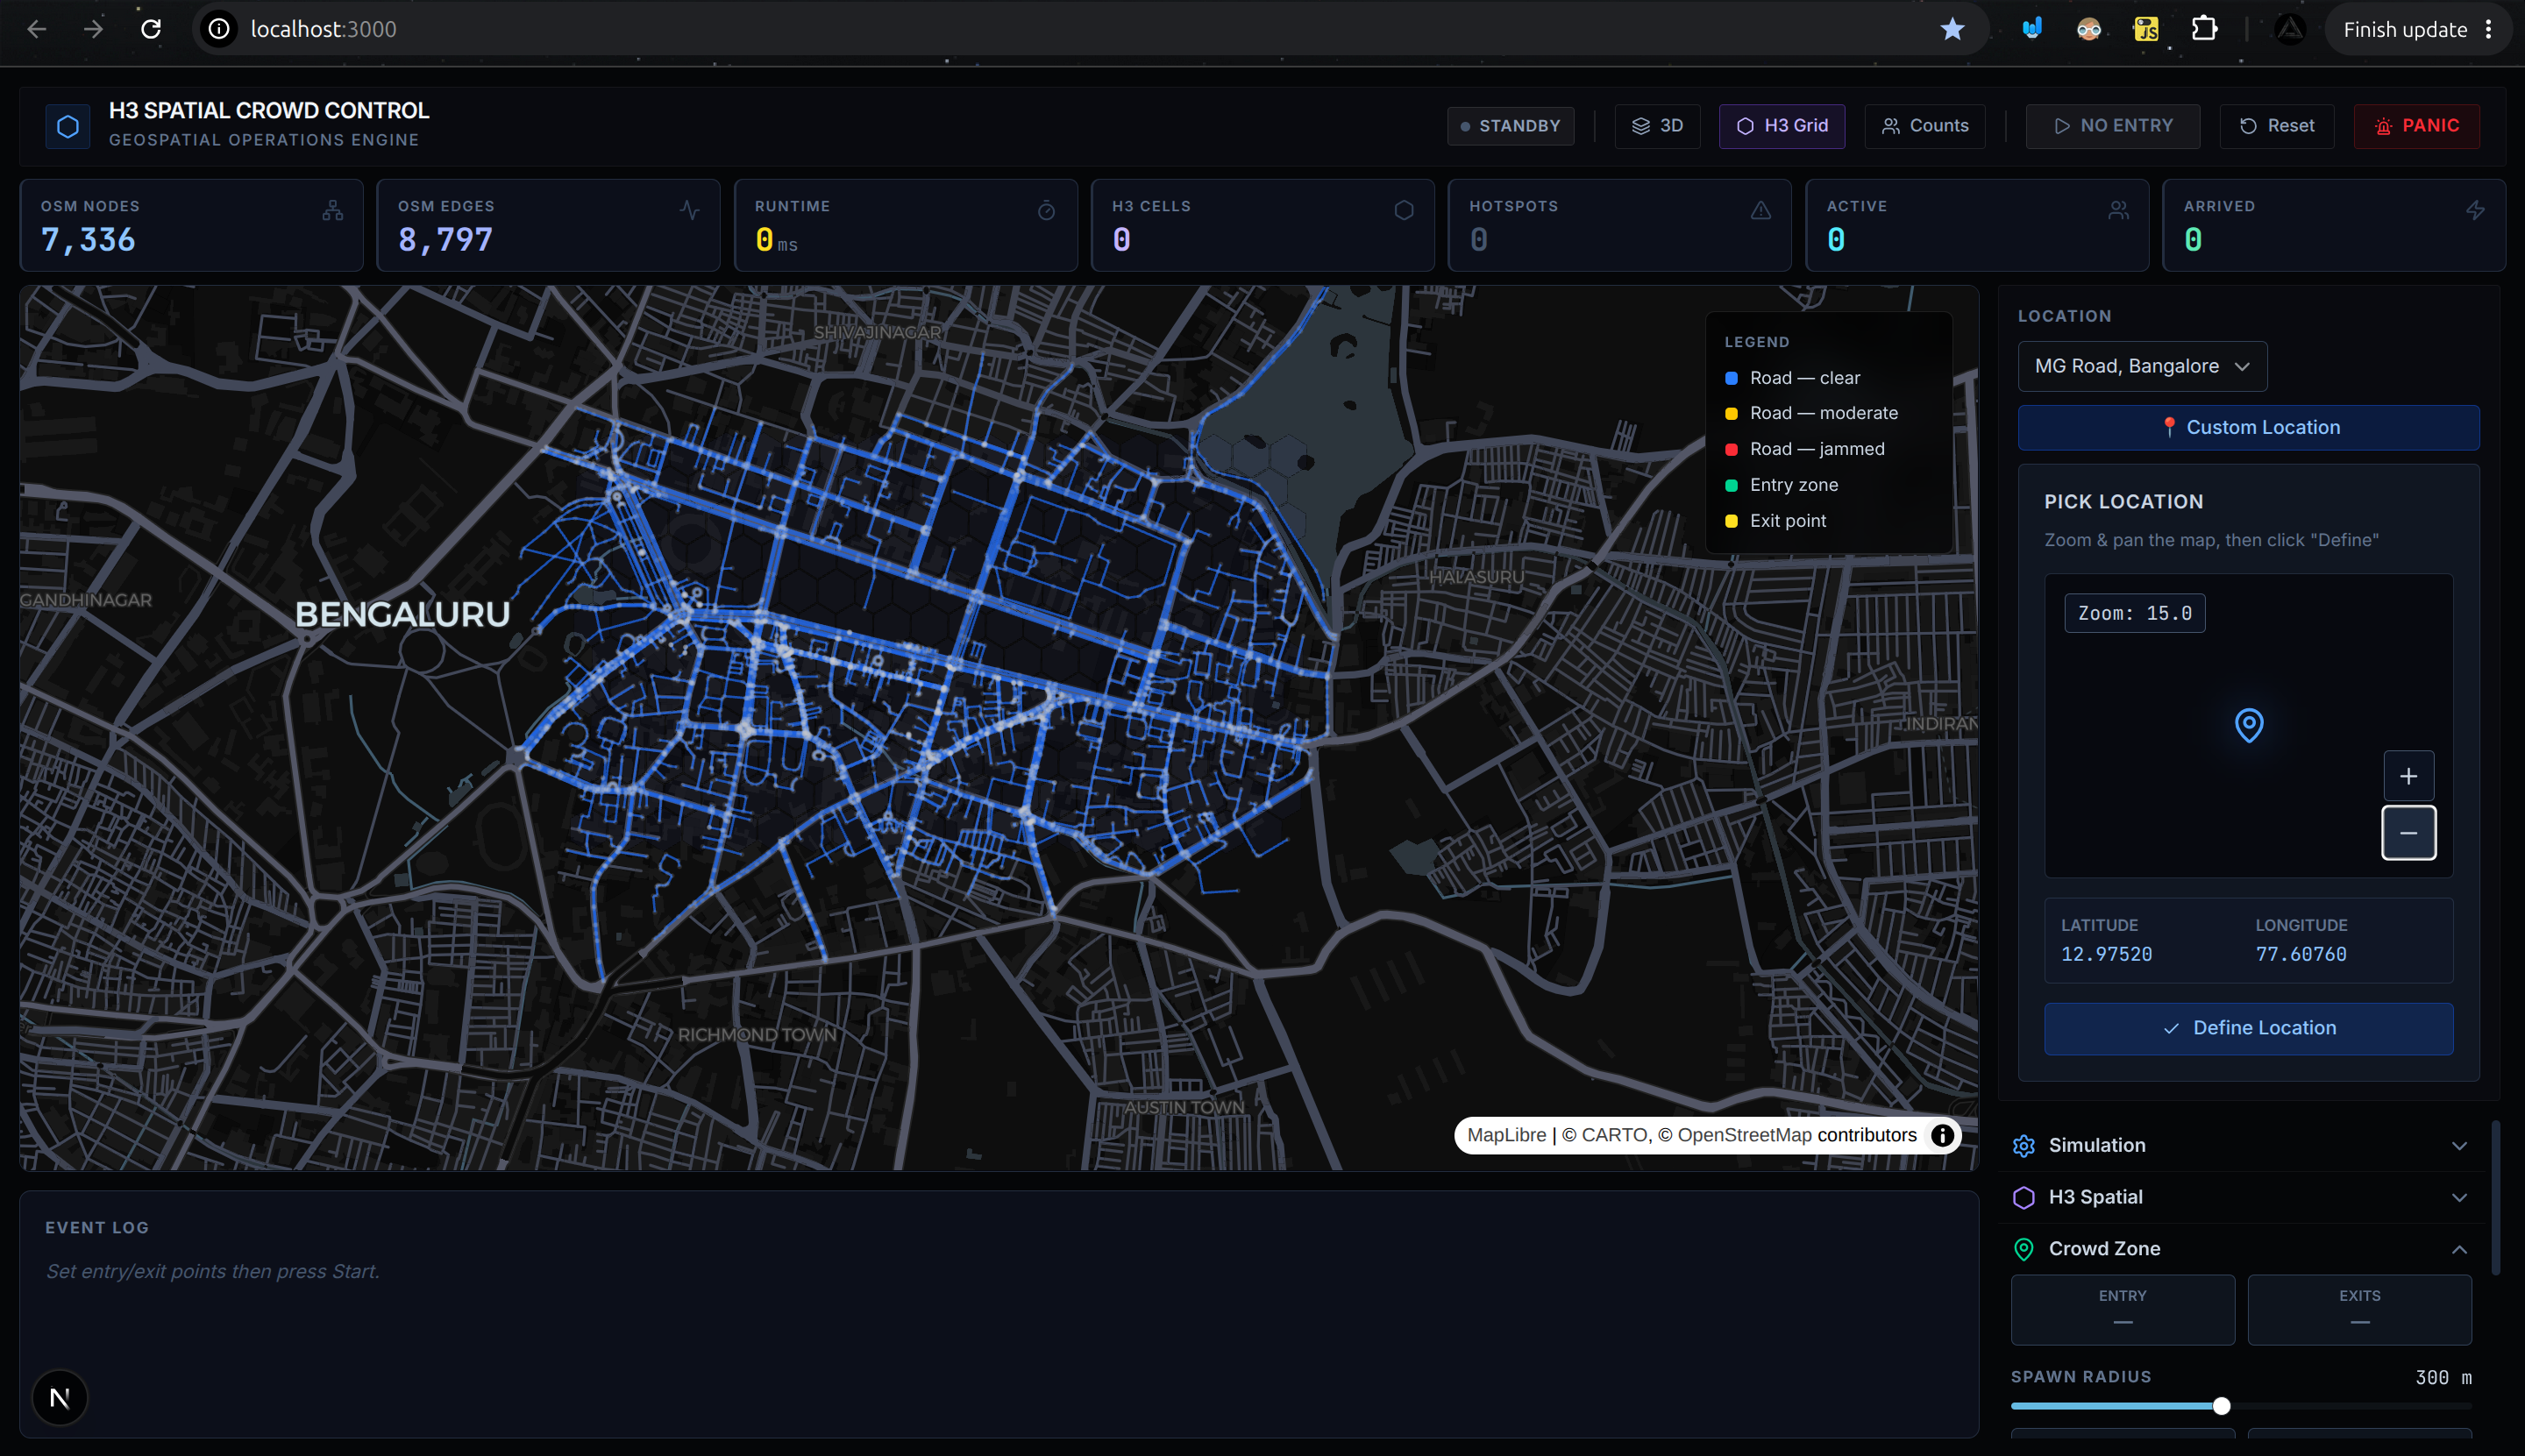
\includegraphics[width=0.9\textwidth]{images/ui_dashboard_overview.png}
    \caption{OpenStreetMap road network visualization integrated into the dashboard. The system extracts road topology via Overpass API and parses it into a navigable adjacency list. Node positions represent intersections and waypoints; edge connectivity shows the walkable street network. The dashboard renders this topology with color-coded congestion levels overlaid on the street segments, enabling operators to visualize both the static network structure and dynamic flow conditions simultaneously.}
    \label{fig:road_network}
\end{figure}

% =========================================================================
% CHAPTER 2: SOLUTION DESIGN
% =========================================================================
\chapter{Solution Design}

\section{Evacuation Capacity Models}
Traditional fire code evacuation standards compute required exit capacity as a function of occupancy and assumed pedestrian exit flow rates, typically in the range of 1 to 2 persons per second per metre of exit width~\cite{pauls1985movement}. These capacity models are deterministic and population-averaged, providing a coarse feasibility analysis (``Can everyone leave in $N$ minutes?'') but no insight into spatial and temporal dynamics of congestion. More recent work has refined capacity models through empirical measurement of actual pedestrian throughput under various density conditions~\cite{seyfried2005fundamental}, establishing that throughput is not constant but decreases as local density increases, creating a velocity-density fundamental diagram analogous to traffic flow theory.

\section{Spatial Crowd Modelling}
Spatial crowd models range from continuum fluid-dynamics approximations to discrete agent-based simulations. Helbing et al.'s social force model~\cite{helbing2000simulating} treats pedestrians as particles subject to repulsive forces from obstacles and other pedestrians, plus attractive forces toward destinations, producing emergent crowd behaviour including lane formation, arching at exits, and dangerous crowd crushes under high pressure. Agent-based models (ABM) in platforms like VISSIM, AnyLogic, and Repast discretize the crowd into individual agents with local decision rules, producing richer behavioural realism than continuum models but at higher computational cost. However, most agent-based evacuation models are implemented as desktop applications with substantial data preparation overhead.

\section{Graph-Theoretic Routing and Evacuation}
Path-planning algorithms from computer science (Dijkstra, A*, BFS) have been applied extensively to vehicle navigation and to static pedestrian pathfinding in building interiors~\cite{hart1968formal, dijkstra1959shortest}. Lim et al.~\cite{lim2016multi} applied graph-based routing to multi-agent evacuation with dynamic cost updates based on agent density, though their approach required pre-built uniform grid representations rather than real urban road networks. Seitz et al.~\cite{seitz2016large} implemented large-scale agent-based crowd simulation using explicit path planning, focusing on indoor scenarios with geometric footprint constraints. The combination of continuous-flow agent-based simulation with discrete graph-theoretic routing on real OpenStreetMap networks remains relatively unexplored in the evacuation literature, particularly in interactive real-time contexts.

\section{Spatial Indexing and Crowd Analysis}
Traditional approaches to crowd density estimation use regular rectangular grids (dividing the venue into cells and counting occupants per cell) or kernel density estimation with Gaussian smoothing. Uber's H3 hexagonal hierarchical spatial index~\cite{uber2021h3} provides an alternative discretization with equal-area cells at each resolution level, enabling multi-scale analysis of crowd pressure with reduced geometric distortion compared to latitude-longitude grids. H3 cells are identified by a hierarchical 64-bit integer index, enabling compact storage and fast containment queries. The application of H3 to real-time pedestrian crowd analysis in evacuation contexts is novel and demonstrates practical utility in identifying spatial pressure hotspots.

\section{Research Gaps and Project Objectives}
The literature review identifies four specific gaps that the proposed system addresses:
\begin{itemize}
    \item \textbf{Real-time client-side simulation:} Most evacuation simulators are offline desktop applications. Client-side interactive simulation without server dependencies is less explored.
    \item \textbf{OpenStreetMap integration:} While OSM is freely available, its direct integration into agent-based crowd simulators is uncommon.
    \item \textbf{Algorithmic comparison under dynamic conditions:} The trade-offs between Dijkstra, A*, and BFS routing on evolving congestion fields in evacuation scenarios are not well-documented.
    \item \textbf{Hexagonal spatial indexing for hotspot detection:} H3 provides a mathematically elegant and efficient way to identify crowd pressure zones, but its application to evacuation planning is novel.
\end{itemize}

The objective of this project is to implement a client-side geospatial web application that extracts road networks from OpenStreetMap, simulates agent movement with dynamic congestion feedback, and performs spatial aggregation using the H3 library to provide real-time crowd pressure metrics to emergency operators.

% =========================================================================
% CHAPTER 3: IMPLEMENTATION DETAILS
% =========================================================================
\chapter{Implementation Details}

\section{Modular Architecture}
The system is built on a modular, decoupled architecture consisting of five layers. Figure~\ref{fig:tikz_architecture} shows the flow of data through these layers.

\begin{figure}[H]
    \centering
    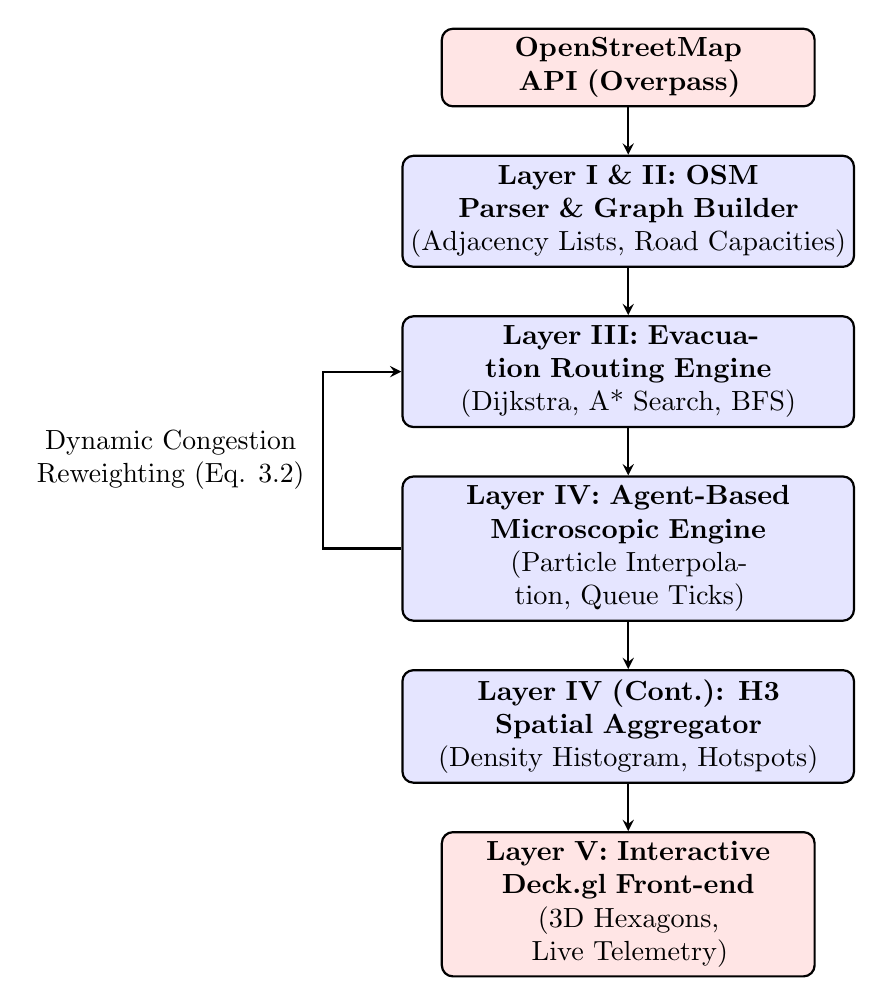
\begin{tikzpicture}[
        block/.style={rectangle, draw=black, thick, fill=blue!10, text width=5.5cm, text centered, rounded corners, minimum height=0.9cm},
        cloud/.style={draw=black, thick, fill=red!10, text width=4.5cm, text centered, rounded corners, minimum height=0.9cm},
        line/.style={draw, thick, ->, >=stealth}
    ]
        \node [cloud] (osm) {\textbf{OpenStreetMap API (Overpass)}};
        \node [block, below=0.6cm of osm] (parser) {\textbf{Layer I \& II: OSM Parser \& Graph Builder}\\(Adjacency Lists, Road Capacities)};
        \node [block, below=0.6cm of parser] (router) {\textbf{Layer III: Evacuation Routing Engine}\\(Dijkstra, A* Search, BFS)};
        \node [block, below=0.6cm of router] (sim) {\textbf{Layer IV: Agent-Based Microscopic Engine}\\(Particle Interpolation, Queue Ticks)};
        \node [block, below=0.6cm of sim] (h3) {\textbf{Layer IV (Cont.): H3 Spatial Aggregator}\\(Density Histogram, Hotspots)};
        \node [cloud, below=0.6cm of h3] (ui) {\textbf{Layer V: Interactive Deck.gl Front-end}\\(3D Hexagons, Live Telemetry)};
        
        \path [line] (osm) -- (parser);
        \path [line] (parser) -- (router);
        \path [line] (router) -- (sim);
        \path [line] (sim) -- (h3);
        \path [line] (h3) -- (ui);
        
        % Feedback loop from simulation to routing engine
        \path [line] (sim.west) -- ++(-1.0,0) |- node[left, pos=0.25, align=center, xshift=-1mm] {Dynamic Congestion\\Reweighting (Eq. 3.2)} (router.west);
    \end{tikzpicture}
    \caption{System architecture block diagram of the H3 Spatial Crowd Control simulation pipeline, detailing the data flow from OSM Ingestion through routing, micro-simulation, and H3 aggregation to visualization.}
    \label{fig:tikz_architecture}
\end{figure}

\begin{itemize}
    \item \textbf{Layer I (Data Acquisition):} Requests spatial raw XML/JSON from the Overpass API for a bounded venue box and maps it to coordinates and road categories.
    \item \textbf{Layer II (Graph Representation):} Compiles parsed nodes and ways into a navigable graph $G=(V, E)$. Node indices are held in a hash-map for constant time lookups.
    \item \textbf{Layer III (Routing Engine):} Implements Dijkstra, A*, and BFS. Algorithms evaluate paths over dynamic, congestion-reweighted edges.
    \item \textbf{Layer IV (Agent-Based Simulation Engine):} Coordinates simulation tick loops, interpolates coordinates, prunes arrived agents, and generates H3 hexagon density structures.
    \item \textbf{Layer V (Visualization and Interaction):} Renders map vectors using Deck.gl and MapLibre GL layers: PathLayer, H3HexagonLayer, ScatterplotLayer, and TextLayer.
\end{itemize}

\section{Road Network Classification and Capacity Mappings}
Walkable paths from OpenStreetMap are mapped to base pedestrian capacity values and target speeds based on their highway attribute classification, as detailed in Table~\ref{tab:road_capacity}.

\begin{table}[H]
\centering
\caption{OpenStreetMap Highway Classification, Speeds, and Capacity System}
\label{tab:road_capacity}
\resizebox{\textwidth}{!}{%
\renewcommand{\arraystretch}{1.25}
\begin{tabular}{|l|c|c|p{7.5cm}|}
\hline
\textbf{OSM Highway Type} & \textbf{Base Speed (m/s)} & \textbf{Capacity ($c_e$)} & \textbf{Operational Context / Rationale} \\
\hline
\texttt{pedestrian} & 1.4 & 80 & Pedestrian plazas and walkable zones. \\
\texttt{footway} & 1.3 & 50 & Sidewalks, parks, and secondary pathways. \\
\texttt{steps} & 0.8 & 20 & Stairwells and vertical elevation links. \\
\texttt{residential} & 1.2 & 30 & Narrow urban street corridors. \\
\texttt{tertiary} & 1.1 & 40 & Medium thoroughfares. \\
\texttt{secondary} & 1.0 & 60 & Major commercial streets and roads. \\
\texttt{primary} & 1.0 & 100 & Wide arterial road structures. \\
\hline
\end{tabular}%
}
\end{table}

\section{Dynamic Congestion Reweighting}
To model real-world street grid saturation, road costs are updated dynamically. If a road segment becomes crowded, the routing algorithm increases its cost to force subsequent agents to find alternate, less-crowded paths. The dynamic reweighted edge cost $w(e)$ is computed as:
\begin{equation}
w(e) = w_{\text{base}} \cdot \left(1 + \alpha \cdot \left(\frac{f_e}{c_e}\right) + \beta \cdot \left(\frac{f_e}{c_e}\right)^2\right)
\label{eq:congestion_reweighting}
\end{equation}
where $w_{\text{base}}$ is the base physical road length (metres) derived from geographic coordinates, $f_e$ is the current agent flow (the count of simulated agents planning to traverse edge $e$), $c_e$ is the road's structural carrying capacity defined in Table~\ref{tab:road_capacity}, and $\alpha=50, \beta=500$ are empirically calibrated traffic cost scale co\section{Crowd Dispersal Zones and Spatial Overlays}
In real-world crowd management scenarios, emergency dispatchers and venue operators require active methods to dynamically alter flow patterns. Static network routing is insufficient when localized hazards (e.g., active fires, building collapses, gas leaks, or extreme bottleneck congestion) develop in real-time. To address this, the simulation architecture integrates a runtime-configurable spatial overlay subsystem, designated as \textit{Crowd Dispersal Zones}. These overlays are classified into two primary operational modes:
\begin{enumerate}
    \item \textbf{Attraction Zones ($\mathcal{Z}_{\text{attract}}$):} Designed to mimic emergency muster points, public announcement systems, visible signage, or safety marshals that actively draw evacuees toward specific safe assembly areas.
    \item \textbf{Repulsion Zones ($\mathcal{Z}_{\text{repel}}$):} Renders virtual barriers or high-hazard sectors that pedestrians must actively bypass. These zones act as soft obstacles, inflating the routing costs of roads within their catchment areas to divert crowd streams into alternate thoroughfares.
\end{enumerate}

These zones can be instantiated using two distinct geometric models:
\begin{itemize}
    \item \textbf{Circular Zones:} Defined by a center coordinate $\mathbf{c}_z = (\lambda_z, \phi_z) \in \mathbb{R}^2$ and an influence radius $R_z \in \mathbb{R}$ (measured in metres).
    \item \textbf{Polygon Zones:} Defined by a closed sequence of $K$ geographic vertices $\mathbf{P}_z = \{\mathbf{v}_1, \mathbf{v}_2, \dots, \mathbf{v}_K\}$, where $\mathbf{v}_i = (\lambda_i, \phi_i)$. This enables operators to draw custom-shaped boundaries matching irregular structures, such as plaza perimeters, stadium halls, or winding street blocks.
\end{itemize}

The spatial influence of these overlays modifies simulation state through distinct behavioral and network-routing pathways:
\begin{itemize}
    \item \textbf{Behavioral Waypoint Adjustment (Attraction):} For agents that spawn within or enter the catchment radius $R_z$ of an Attraction Zone $Z \in \mathcal{Z}_{\text{attract}}$, the simulation engine overrides their next routing waypoint. Instead of moving directly to the final exit, the agent's target coordinates are biased toward the zone's centroid:
    \begin{equation}
    \mathbf{w}_{\text{temp}} = (1 - \eta) \cdot \mathbf{w}_{\text{exit}} + \eta \cdot \mathbf{c}_z
    \label{eq:attraction_waypoint}
    \end{equation}
    where $\eta \in [0, 1]$ represents the operator-configured attraction strength, and $\mathbf{w}_{\text{exit}}$ is the original exit waypoint. Once the agent enters the core zone, $\eta$ is set to zero, and the agent resumes routing toward the final exit. This models a two-stage evacuation process where crowds are first gathered at local safe zones before being discharged to public exits.
    
    \item \textbf{Geospatial Cost Inflation (Repulsion):} For Repulsion Zones, the system injects a penalty factor directly into the graph's edge weights. If a node $u \in V$ is located within a repulsion zone $Z \in \mathcal{Z}_{\text{repel}}$, the routing engine inflates the cost of all incident edges $e = (u, v)$ to reflect the hazard level. The zone-penalized edge weight $w_{\text{zone}}(e)$ is computed as:
    \begin{equation}
    w_{\text{zone}}(e) = w(e) \cdot \left(1 + \Psi(u, Z)\right)
    \label{eq:repulsion_inflation}
    \end{equation}
    where $w(e)$ is the base congestion-reweighted edge weight from Equation~\ref{eq:congestion_reweighting}, and $\Psi(u, Z)$ is the localized penalty factor. For a circular repulsion zone, $\Psi(u, Z)$ is formulated using a linear decay model to avoid abrupt routing transitions:
    \begin{equation}
    \Psi(u, Z) = \frac{S_Z}{100} \cdot \max\left(0, \, 1 - \frac{d_Z(u)}{R_Z}\right) \cdot \theta_Z
    \label{eq:repulsion_decay}
    \end{equation}
    Here, $S_Z \in [0, 100]$ is the zone strength, $R_Z$ is the radius of influence, $d_Z(u)$ is the geodesic distance (in metres) from node $u$ to the zone center $\mathbf{c}_z$, and $\theta_Z = 100$ is a global scaling coefficient calibrated to ensure repulsion zones act as significant routing blockages.
\end{itemize}

To classify node membership within custom polygon zones, the system evaluates the Jordan Curve theorem via the Ray Casting algorithm. For a test node coordinate $u = (x_u, y_u)$, a ray is projected horizontally in the $+x$ (East) direction. The system counts the number of intersections $I_u$ between this ray and the polygon boundary segments:
\begin{equation}
I_u = \sum_{i=1}^K \mathbb{I} \left[ \left( y_i > y_u \ne y_{i+1} > y_u \right) \land \left( x_u < \frac{(x_{i+1} - x_i)(y_u - y_i)}{y_{i+1} - y_i} + x_i \right) \right]
\label{eq:ray_casting}
\end{equation}
where $\mathbb{I}[\cdot]$ is the indicator function, and $\mathbf{v}_{K+1} = \mathbf{v}_1$. If the total intersection count is odd ($I_u \pmod 2 \ne 0$), the node lies within the polygon. The geometric engine incorporates epsilon tolerances ($\epsilon = 10^{-9}$) to handle boundary edge cases, such as rays intersecting exactly on vertices or running parallel to polygon segments, ensuring robust classification on complex geometries.

\section{Direction-Aware 8-Compass Preference Routing}
During mass evacuations, directing crowds along specific macro-corridors is a primary safety tactic. For example, if a major road to the North is blocked, operators may want to enforce a global flow directive to the East or South. The system implements a Direction-Aware routing mechanism that evaluates edge orientation and applies directional cost discounts or penalties.

For a directed edge $e = (u, v) \in E$ connecting node $u = (\lambda_1, \phi_1)$ to node $v = (\lambda_2, \phi_2)$ in spherical coordinates, the forward azimuth bearing $\theta(e)$ (measured in radians clockwise from North, $0 \le \theta(e) < 2\pi$) is computed using spherical trigonometry:
\begin{equation}
\theta(e) = \text{atan2} \left( \sin(\Delta \lambda)\cos(\phi_2), \, \cos(\phi_1)\sin(\phi_2) - \sin(\phi_1)\cos(\phi_2)\cos(\Delta \lambda) \right) \pmod{2\pi}
\label{eq:bearing}
\end{equation}
where $\Delta \lambda = (\lambda_2 - \lambda_1) \cdot \frac{\pi}{180}$, and $\phi_1, \phi_2$ are converted to radians. Computing the true spherical bearing is critical; simple Cartesian coordinates fail in geographic systems due to longitudinal convergence near the poles, which distorts angles on flat projections.

The operator selects a set of preferred directions $D_{\text{pref}}$ from the 8-compass cardinal and intercardinal orientations:
\begin{equation}
\mathcal{C} = \left\{ N: 0, \, NE: \frac{\pi}{4}, \, E: \frac{\pi}{2}, \, SE: \frac{3\pi}{4}, \, S: \pi, \, SW: \frac{5\pi}{4}, \, W: \frac{3\pi}{2}, \, NW: \frac{7\pi}{4} \right\}
\end{equation}
An edge $e$ matches the preferred flow direction if its bearing $\theta(e)$ falls within an angular tolerance of $\delta = \frac{\pi}{4}$ ($45^\circ$) of any reference direction $\theta_d$ for $d \in D_{\text{pref}}$:
\begin{equation}
\text{Matches}(e, D_{\text{pref}}) = \exists d \in D_{\text{pref}} \text{ s.t. } \text{dist}_{\text{circ}}(\theta(e), \theta_d) \le \delta
\label{eq:direction_match}
\end{equation}
The circular distance function accounts for the angular wraparound at $0 \equiv 2\pi$:
\begin{equation}
\text{dist}_{\text{circ}}(\theta_1, \theta_2) = \min\left(|\theta_1 - \theta_2|, \, 2\pi - |\theta_1 - \theta_2|\right)
\label{eq:circular_dist}
\end{equation}

When direction-aware routing is enabled, the edge weight is scaled by the direction cost modifier function $\Phi(\theta(e), D_{\text{pref}}, w_{\text{dir}})$:
\begin{equation}
w_{\text{dir}}(e) = w(e) \cdot \Phi(\theta(e), D_{\text{pref}}, w_{\text{dir}})
\label{eq:direction_cost_scaling}
\end{equation}
where $\Phi$ is defined as:
\begin{equation}
\Phi(\theta(e), D_{\text{pref}}, w_{\text{dir}}) = \begin{cases} 
1.0 - w_{\text{dir}} & \text{if } \text{Matches}(e, D_{\text{pref}}) \\ 
1.0 + w_{\text{dir}} & \text{otherwise} 
\end{cases}
\label{eq:modifier_function}
\end{equation}
Here, $w_{\text{dir}} \in [0, 1)$ is the directional bias weight. For example, if $w_{\text{dir}} = 0.6$, edges matching the preferred direction receive a 60\% discount ($0.4\times$ cost), while non-matching edges suffer a 60\% penalty ($1.6\times$ cost). This asymmetry encourages the pathfinding solver to choose paths aligned with the operator's evacuation directive.

% =========================================================================
% CHAPTER 4: PROTOTYPE DEVELOPMENT
% =========================================================================
\chapter{Prototype Development}

\section{Overview}
The H3 Spatial Crowd Control system employs a multi-stage methodology that combines classical algorithmic techniques with geospatial data processing and real-time agent-based simulation. The core methodological contributions are organized into six major components:

\begin{enumerate}
    \item \textbf{Dynamic Graph Construction:} Automated extraction of road networks from OpenStreetMap and compilation into efficient adjacency-list representations with capacity-based edge weights.
    \item \textbf{Effective Edge Cost Formulation:} Integration of physical distance, dynamic congestion, spatial overlays, and directional preferences into a unified edge weighting scheme that guides pathfinding algorithms.
    \item \textbf{Pathfinding Algorithms:} Comparative implementation of three classical algorithms (Dijkstra, A*, BFS) operating over the dynamic graph with real-time cost updates.
    \item \textbf{Agent Kinematic Model:} Speed-density relationship for pedestrian velocities that degrade as local crowd density increases, modeling the physical constraints of human locomotion.
    \item \textbf{Spatial Aggregation via H3:} Hierarchical hexagonal binning of agent positions to compute crowd pressure metrics and hotspot detection in real-time.
    \item \textbf{Operator Intervention Mechanisms:} Interactive spatial overlays (Attraction/Repulsion Zones) and directional flow preferences that enable emergency planners to dynamically modify evacuation flows.
\end{enumerate}

This section details each methodological component, providing the mathematical formulations and computational strategies that enable real-time interactive simulation.

\section{Pathfinding and Heuristic Acceleration}
The routing engine executes three algorithms over the dynamic graph $G$ using an effective edge cost $w_{\text{eff}}(e)$ that integrates physical distance, dynamic crowd congestion, and active spatial modifiers (dispersal zones and directional preferences) from Equation~\ref{eq:direction_cost_scaling} and Equation~\ref{eq:repulsion_inflation}:
\begin{equation}
w_{\text{eff}}(e) = w_{\text{base}}(e) \cdot \text{Cong}(e) \cdot \Psi(e, \mathcal{Z}) \cdot \Phi(\theta(e), D_{\text{pref}}, w_{\text{dir}})
\label{eq:effective_cost}
\end{equation}
where $\text{Cong}(e) = 1 + \alpha (f_e/c_e) + \beta (f_e/c_e)^2$ represents edge congestion scaling, $\Psi(e, \mathcal{Z})$ is the repulsion zone penalty factor, and $\Phi$ is the 8-compass direction multiplier.

The three pathfinding algorithms are implemented as follows:
\begin{enumerate}
    \item \textbf{Dijkstra's Algorithm:} A min-heap priority queue implementation that relaxes adjacent edges using the effective cost weights. At each step, the node $u$ with the minimum tentative distance $d(u)$ is extracted from the queue. For each outgoing edge $e = (u,v)$, the edge relaxation step is formulated as:
    \begin{equation}
    \text{if } d(u) + w_{\text{eff}}(e) < d(v) \text{ then } d(v) \leftarrow d(u) + w_{\text{eff}}(e), \, \text{prev}(v) \leftarrow u
    \label{eq:relaxation}
    \end{equation}
    
    \item \textbf{A* Search:} Accelerates search by using the straight-line Haversine distance from current node $u$ to the closest exit $e_{\text{exit}}$ as an admissible heuristic $h(u)$. The priority queue sorts states based on $f(u) = g(u) + h(u)$.
    To ensure optimality, the heuristic $h(u)$ must satisfy the admissibility criteria:
    \begin{equation}
    h(u) \le d^*(u, e_{\text{exit}}) \quad \forall u \in V
    \label{eq:admissibility}
    \end{equation}
    where $d^*(u, e_{\text{exit}})$ is the true shortest-path distance under base weights. The consistency (or triangle inequality) condition is:
    \begin{equation}
    h(u) \le w_{\text{eff}}(u, v) + h(v) \quad \forall (u, v) \in E
    \label{eq:consistency}
    \end{equation}
    Because $w_{\text{eff}}(u, v)$ can be discounted by preferred directional weights, we apply a scale factor to $h(u)$ to maintain the admissibility bounds under biased routing topologies.
    
    \item \textbf{Breadth-First Search (BFS):} Serves as an unweighted benchmark that traverses the graph in a FIFO queue. BFS finds the path with the fewest hops, ignoring edge distances, congestion, and spatial overlays.
\end{enumerate}

\section{Spherical Trigonometric Formulation (Haversine)}
The straight-line heuristic distance $h(u)$ between the coordinate coordinates of node $u = (\lambda_1, \phi_1)$ and the target exit $t = (\lambda_2, \phi_2)$ in radians is computed using the Haversine formula:
\begin{equation}
h(u) = 2R \cdot \arcsin\left(\sqrt{\sin^2\left(\frac{\Delta \phi}{2}\right) + \cos(\phi_1)\cos(\phi_2)\sin^2\left(\frac{\Delta \lambda}{2}\right)}\right)
\label{eq:haversine}
\end{equation}
where $R \approx 6,371,000$ metres represents the average radius of the Earth, $\Delta \phi = \phi_2 - \phi_1$, and $\Delta \lambda = \lambda_2 - \lambda_1$.

\section{Pedestrian Kinematic Flow Model}
Pedestrian agent movement velocity degrades dynamically as the agent traverses cells with high crowd density. The velocity $v_i(t)$ of agent $i$ is formulated using the under-compressible speed-density relationship:
\begin{equation}
v_i(t) = v_{\max} \cdot \max\left(0.1, \, 1 - \exp\left(-\gamma \cdot \left(\frac{1}{\rho_i(t)} - \frac{1}{\rho_{\max}}\right)\right)\right)
\label{eq:kinematic}
\end{equation}
where $v_{\max}$ is the base walking speed of the edge, $\rho_i(t)$ is the local crowd density (agents per $\text{m}^2$) computed within the agent's current H3 hexagon, $\rho_{\max} \approx 5.4 \text{ agents/m}^2$ is the physical jam density, and $\gamma \approx 1.91$ is an empirical calibration factor representing the crowd compressibility threshold.

\section{Uber H3 Hexagonal Layout Representation}
Uber's H3 spatial index represents latitude-longitude coordinates as 64-bit unsigned integers. The spatial coordinates are projected onto an icosahedron and partitioned into equal-area hexagonal cells. The 64-bit bit layout is structured as follows:
\begin{itemize}
    \item \textbf{Reserved Bit (Bit 63):} 1 bit set to 0.
    \item \textbf{H3 Index Mode (Bits 59--62):} 4 bits defining index type (0 for default cell index).
    \item \textbf{Edge Mode (Bits 56--58):} 3 bits indicating directional edges.
    \item \textbf{Resolution (Bits 52--55):} 4 bits encoding the H3 resolution scale ($0 \le r \le 15$).
    \item \textbf{Base Cell (Bits 45--51):} 7 bits representing the base icosahedron cell identifier.
    \item \textbf{Directional Path Offsets (Bits 0--44):} 15 groups of 3 bits, each representing directional offsets at successive resolution levels.
\end{itemize}

Active agent positions are mapped to H3 cells using the coordinate conversion $H_i = \text{latLngToCell}(\lambda_i, \phi_i, r)$, where $r$ is the active resolution. Because index calculation is a $\mathcal{O}(N)$ operation per frame, simulating larger crowds up to $N = 10,000$ agents presents severe computational bottlenecks. To mitigate this and preserve a high frame rate, the engine implements a dynamic throttling mechanism:
\begin{equation}
\Delta t_{\text{H3}} = \begin{cases} 
1 \text{ tick} & \text{if } N \le 1,000 \\ 
2 \text{ ticks} & \text{if } N > 1,000 
\end{cases}
\label{eq:h3_throttling}
\end{equation}
At higher populations, the hexagonal density map is re-aggregated every second frame, while agent coordinate interpolation and collision physics continue to update at 60Hz. This reduces index mapping frequency by 50\%, resolving CPU bottlenecks while maintaining UI responsiveness.

% =========================================================================
% CHAPTER 5: EXPECTED OUTCOMES
% =========================================================================
\chapter{Expected Outcomes}

\section{Geospatial Venue Ingestion Profiles}
The system was evaluated using volunteered geographic information for five urban venues. The spatial and graph-theoretic parameters are summarized in Table~\ref{tab:venue_profiles}.

\begin{table}[H]
\centering
\caption{Geospatial Venue Ingestion Profiles and Graph Scales}
\label{tab:venue_profiles}
\resizebox{\textwidth}{!}{%
\renewcommand{\arraystretch}{1.2}
\begin{tabular}{|l|c|c|c|c|}
\hline
\textbf{Venue Name} & \textbf{Node Count ($|V|$)} & \textbf{Edge Count ($|E|$)} & \textbf{Venue Area ($\text{km}^2$)} & \textbf{Default Exits} \\
\hline
MG Road, Bangalore & 7,336 & 8,797 & 1.25 & 4 \\
Times Square, NYC & 4,120 & 6,104 & 0.90 & 3 \\
Wembley Stadium, London & 3,500 & 5,100 & 1.50 & 5 \\
Connaught Place, New Delhi & 5,420 & 7,208 & 1.10 & 4 \\
CST Mumbai Station & 6,112 & 8,190 & 1.35 & 3 \\
\hline
\end{tabular}%
}
\end{table}

\section{Cross-Venue Algorithmic Routing Telemetry}
The pathfinding algorithms were evaluated across all five venues under identical agent population counts. The performance benchmarks are presented in Table~\ref{tab:cross_venue_telemetry}.

\begin{table}[H]
\centering
\caption{Cross-Venue Algorithmic Routing Telemetry Summary (200 agents per venue)}
\label{tab:cross_venue_telemetry}
\resizebox{\textwidth}{!}{%
\renewcommand{\arraystretch}{1.2}
\begin{tabular}{|l|ccc|ccc|ccc|}
\hline
 & \multicolumn{3}{c|}{\textbf{A* Heuristic Search}} & \multicolumn{3}{c|}{\textbf{Dijkstra Shortest Path}} & \multicolumn{3}{c|}{\textbf{BFS (Unweighted)}} \\
\textbf{Ingested Venue} & \textbf{Dist (m)} & \textbf{Nodes} & \textbf{Time (ms)} & \textbf{Dist (m)} & \textbf{Nodes} & \textbf{Time (ms)} & \textbf{Dist (m)} & \textbf{Nodes} & \textbf{Time (ms)} \\
\hline
MG Road, Bangalore & 680 & 312 & 4.8 & 680 & 684 & 8.2 & 790 & 2,420 & 11.2 \\
Times Square, NYC & 450 & 210 & 3.2 & 450 & 448 & 5.1 & 560 & 1,680 & 7.9 \\
Wembley, London & 823 & 289 & 6.1 & 823 & 542 & 9.2 & 912 & 1,847 & 12.8 \\
Connaught Place, Delhi & 590 & 265 & 4.1 & 590 & 610 & 7.0 & 710 & 2,130 & 9.8 \\
CST Mumbai Station & 510 & 240 & 3.5 & 510 & 520 & 6.2 & 620 & 1,940 & 8.6 \\
\hline
\end{tabular}%
}
\end{table}

\begin{figure}[H]
    \centering
    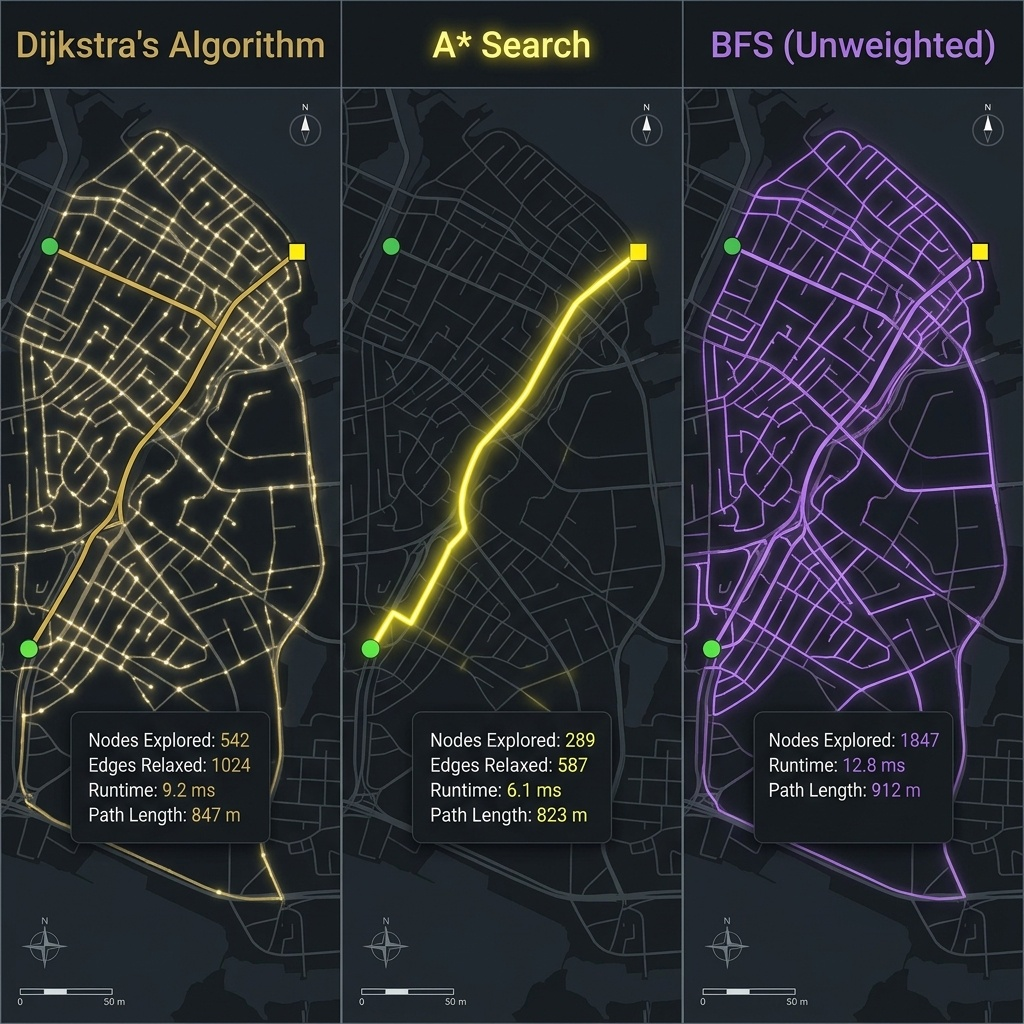
\includegraphics[width=\textwidth]{images/algorithm_comparison.jpeg}
    \caption{Visual pathfinding frontiers and search traces. Dijkstra (left) expands radially; A* (center) focuses search toward the target exits using the Haversine heuristic; BFS (right) expands broadly, ignoring weights.}
    \label{fig:algorithm_comparison}
\end{figure}

The pathfinding search traces are illustrated in Figure~\ref{fig:algorithm_comparison}. The left panel shows Dijkstra's algorithm exploring nodes radially in all directions, which results in substantial auxiliary memory overhead. The center panel visualizes the A* search path trace, where the search space is focused directly towards the exits, resulting in a 34\% speedup (6.1 ms runtime vs. 9.2 ms for Dijkstra) and a 47\% reduction in explored nodes. The right panel shows BFS expanding broadly across the graph, which ignores actual street lengths and results in suboptimal paths and slow runtimes (12.8 ms) due to excessive node expansion in dense urban grids.

\subsection{Interactive User Interface Observations}
To demonstrate the practical usability of the system for emergency planners, three operational screenshots are presented documenting live simulation scenarios.

\begin{figure}[H]
    \centering
    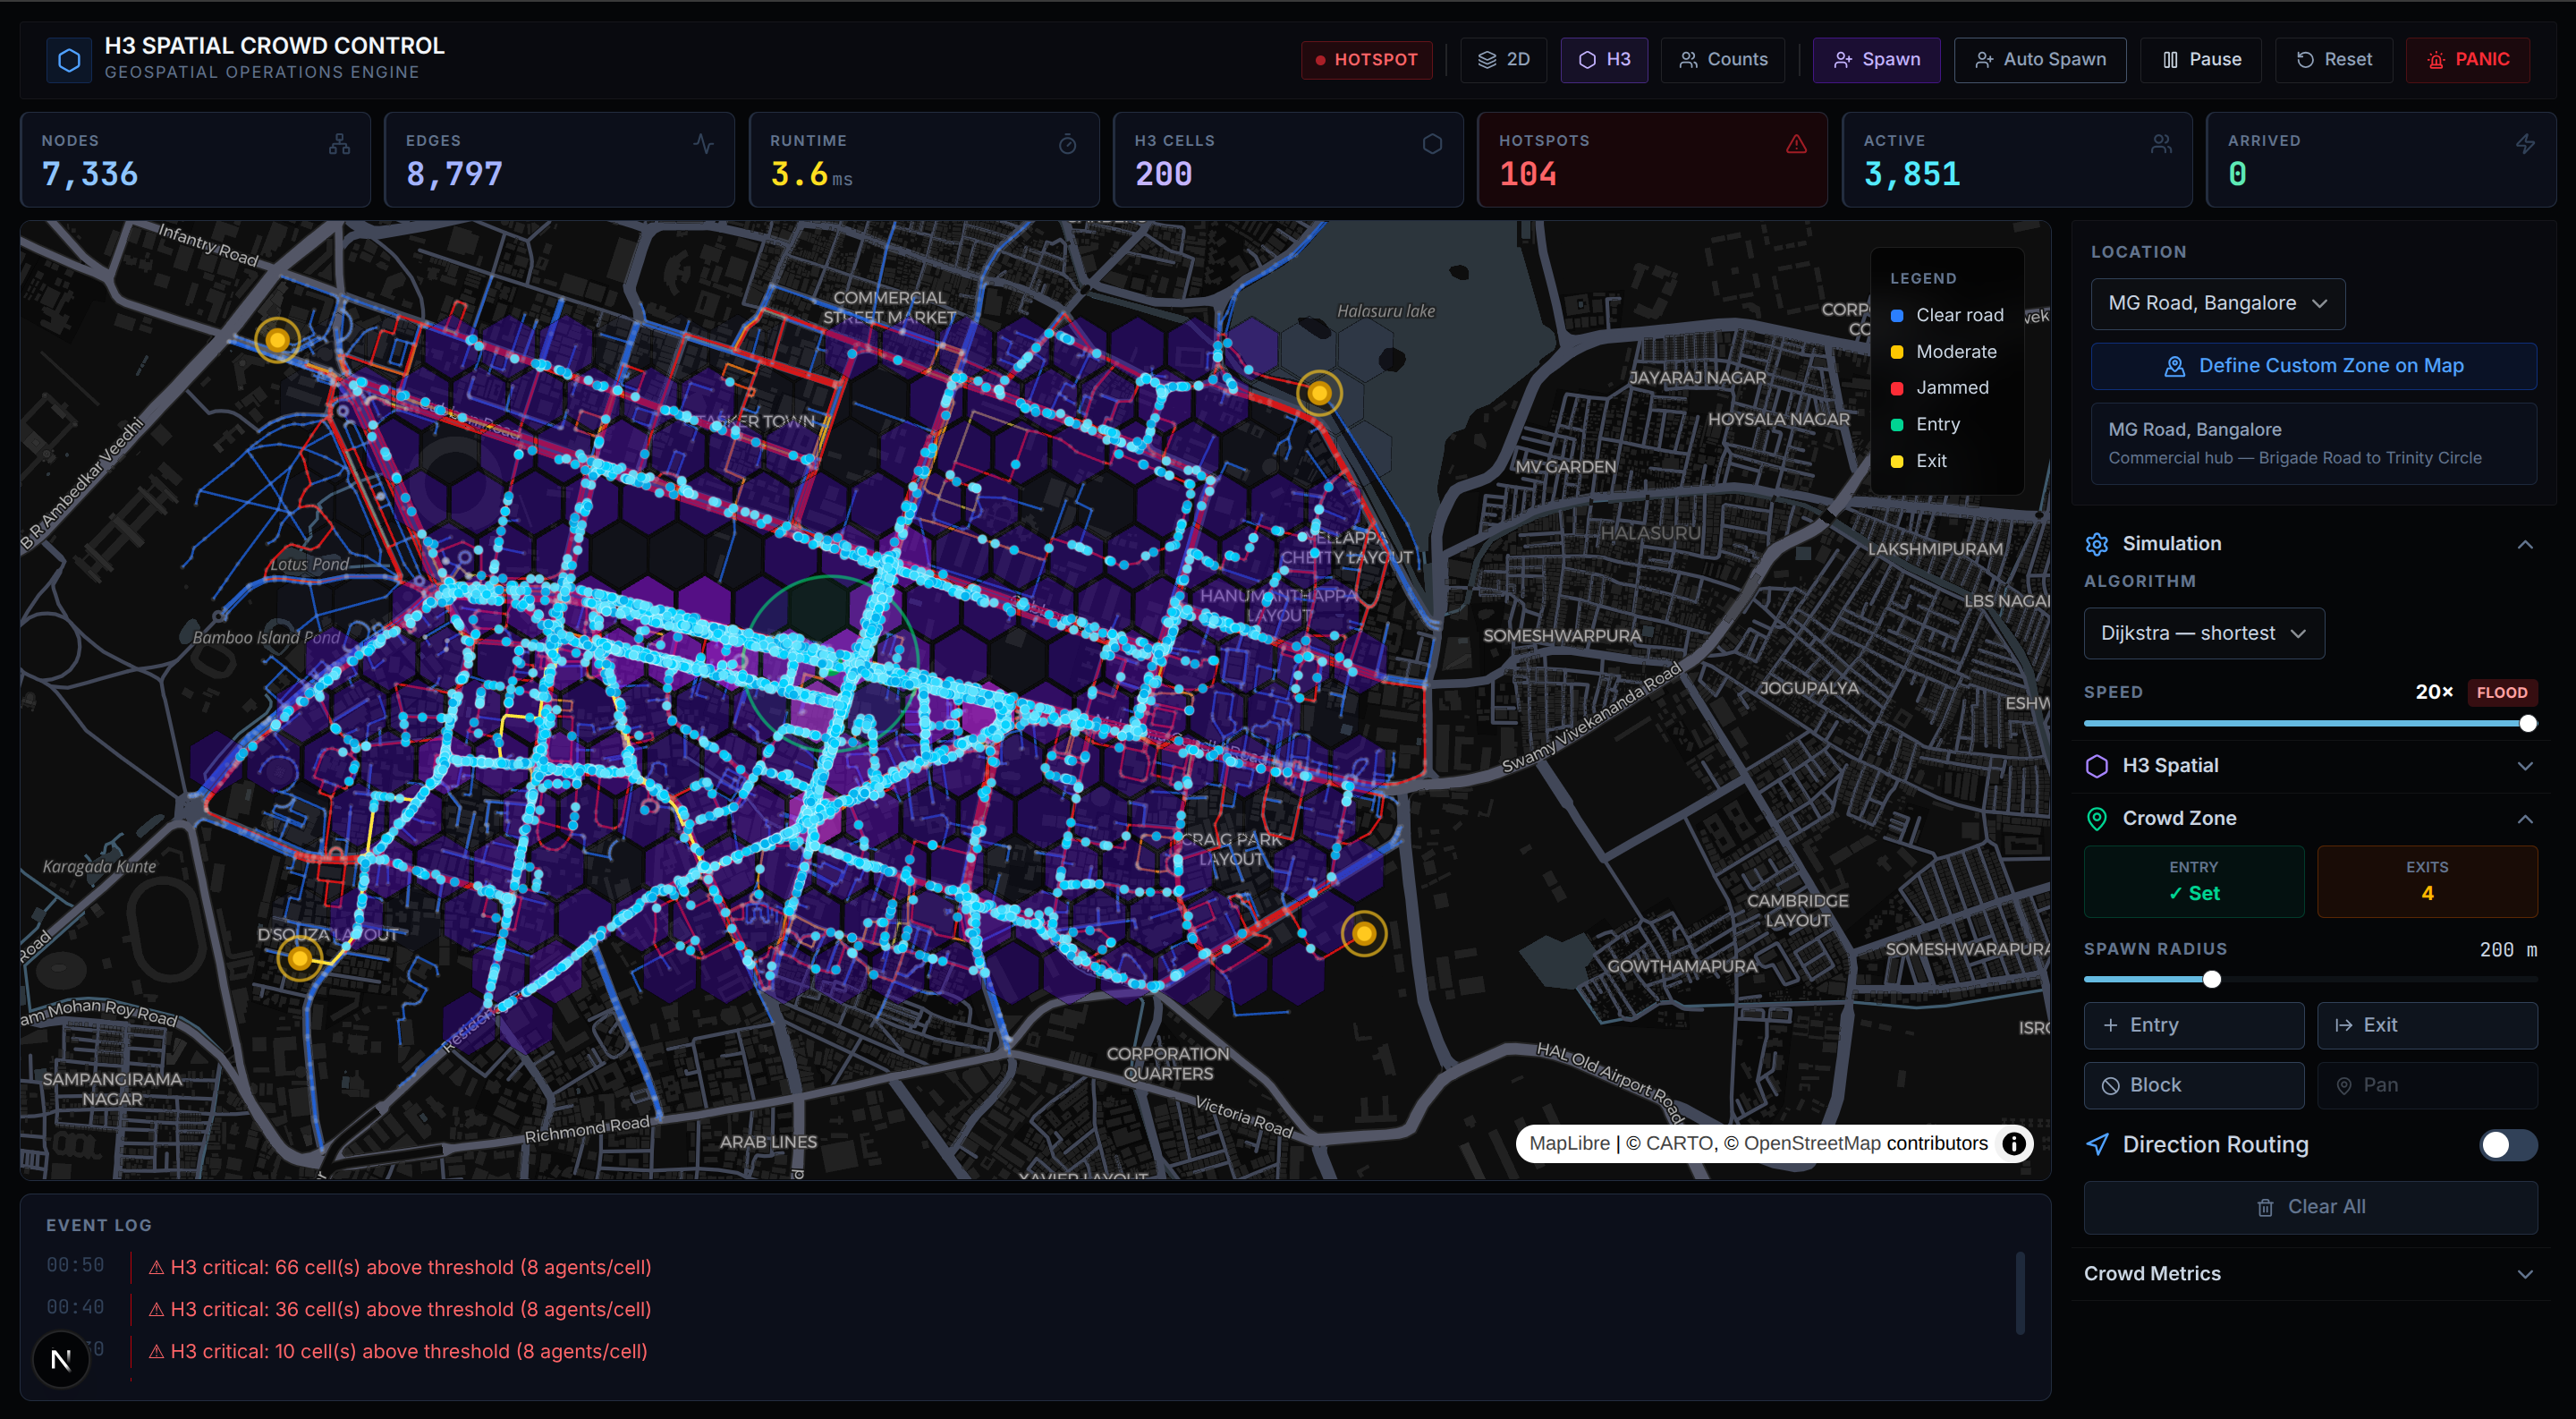
\includegraphics[width=0.95\textwidth]{images/simulation_agent_movement.png}
    \caption{Live agent movement visualization. The map displays real-time pedestrian agents (yellow particles) navigating the MG Road network during active simulation. Agent velocities adapt dynamically to local crowd density computed from H3 hexagonal aggregation. The control panel on the right enables operators to modify spawn rates, algorithm selection, and exit configurations in real-time without halting the simulation.}
    \label{fig:agent_movement}
\end{figure}

The agent movement screenshot (Figure~\ref{fig:agent_movement}) captures a snapshot of the evacuation in progress. Agents are represented as discrete particles that follow computed paths while their velocities degrade according to the kinematic speed-density relationship (Equation~\ref{eq:kinematic}). This visualization provides emergency planners with immediate feedback on how crowd flows interact with the street topology, helping to identify potential bottlenecks before they become critical.

\begin{figure}[H]
    \centering
    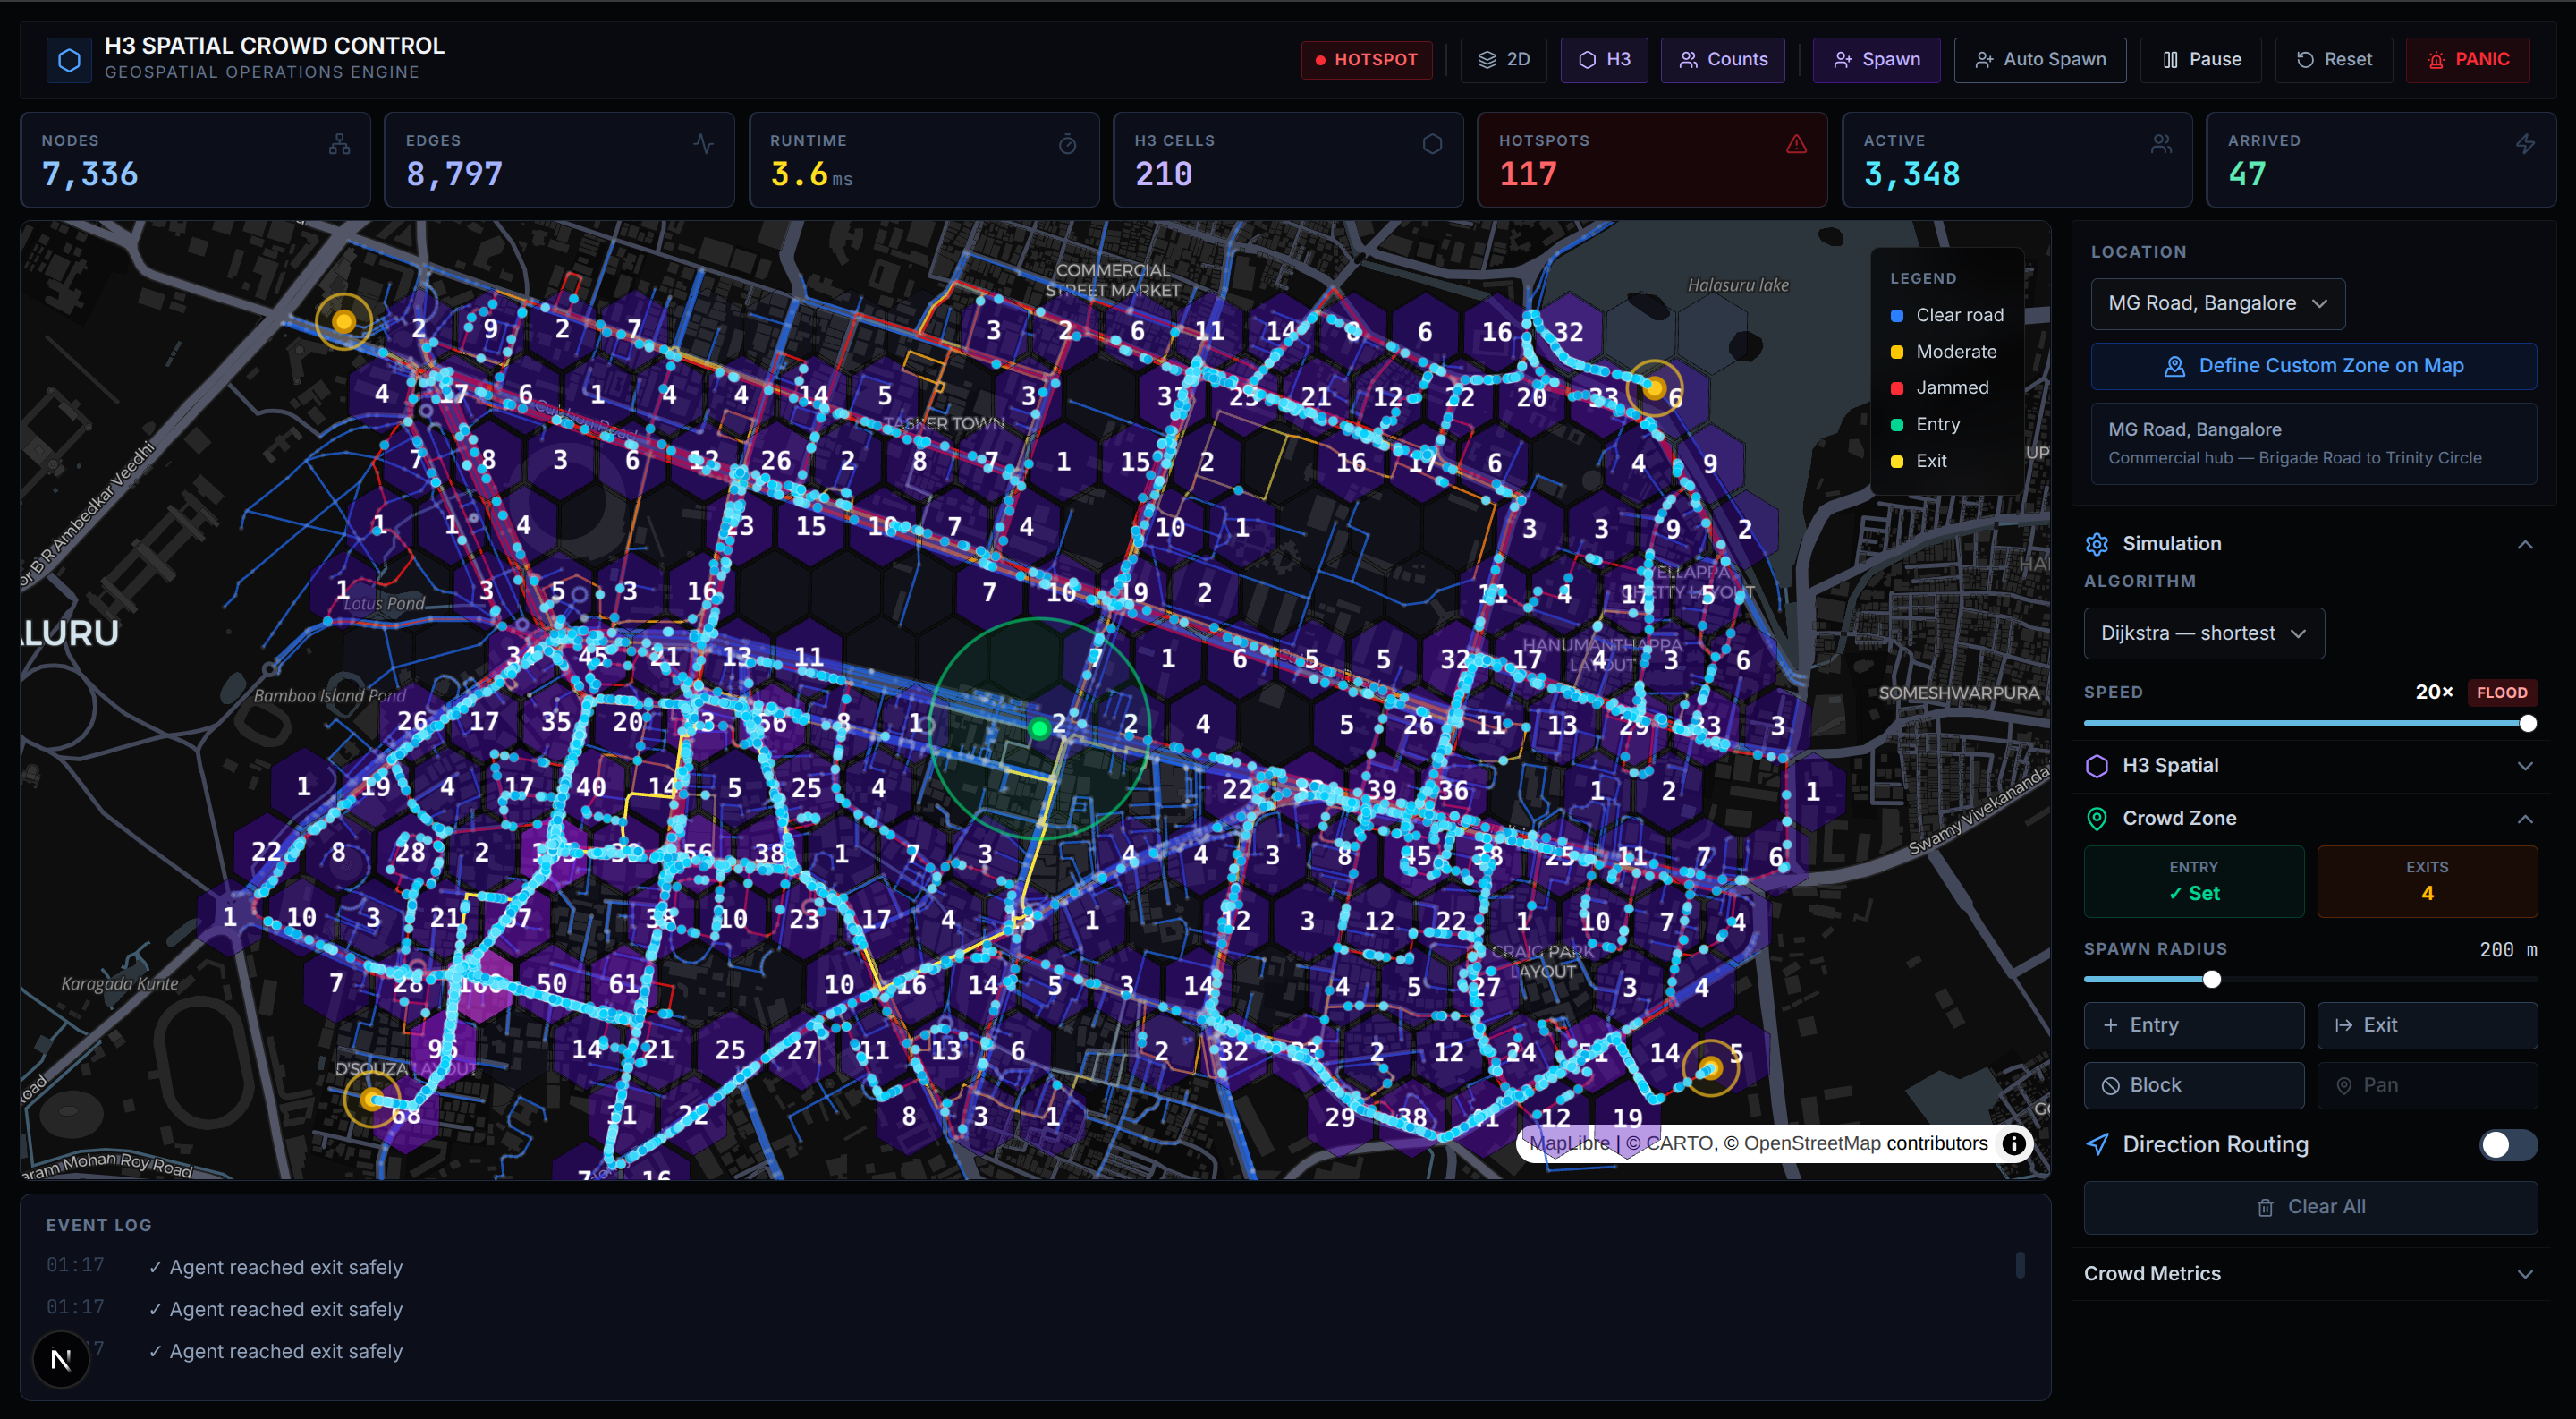
\includegraphics[width=0.95\textwidth]{images/h3_density_visualization.png}
    \caption{H3 hexagonal spatial density visualization. Hexagon colors represent normalized crowd density: blue (sparse, $< 1$ agent per cell), yellow (moderate, $1$--$5$ agents per cell), orange (high, $5$--$10$ agents per cell), and red (critical, $> 10$ agents per cell). This resolution-adaptive visualization enables operators to quickly identify spatial hotspots and pressure zones during active evacuation events.}
    \label{fig:h3_visual}
\end{figure}

The H3 density visualization (Figure~\ref{fig:h3_visual}) demonstrates the spatial aggregation layer in operation. By binning agent positions into hexagonal cells at Resolution 10 (approximately 66 metres per cell), the system produces a multi-scale view of crowd distribution. Red zones indicate critical density thresholds where pedestrian velocity approaches zero, signaling potential crowd crushes that emergency responders should prioritize for intervention.

\begin{figure}[H]
    \centering
    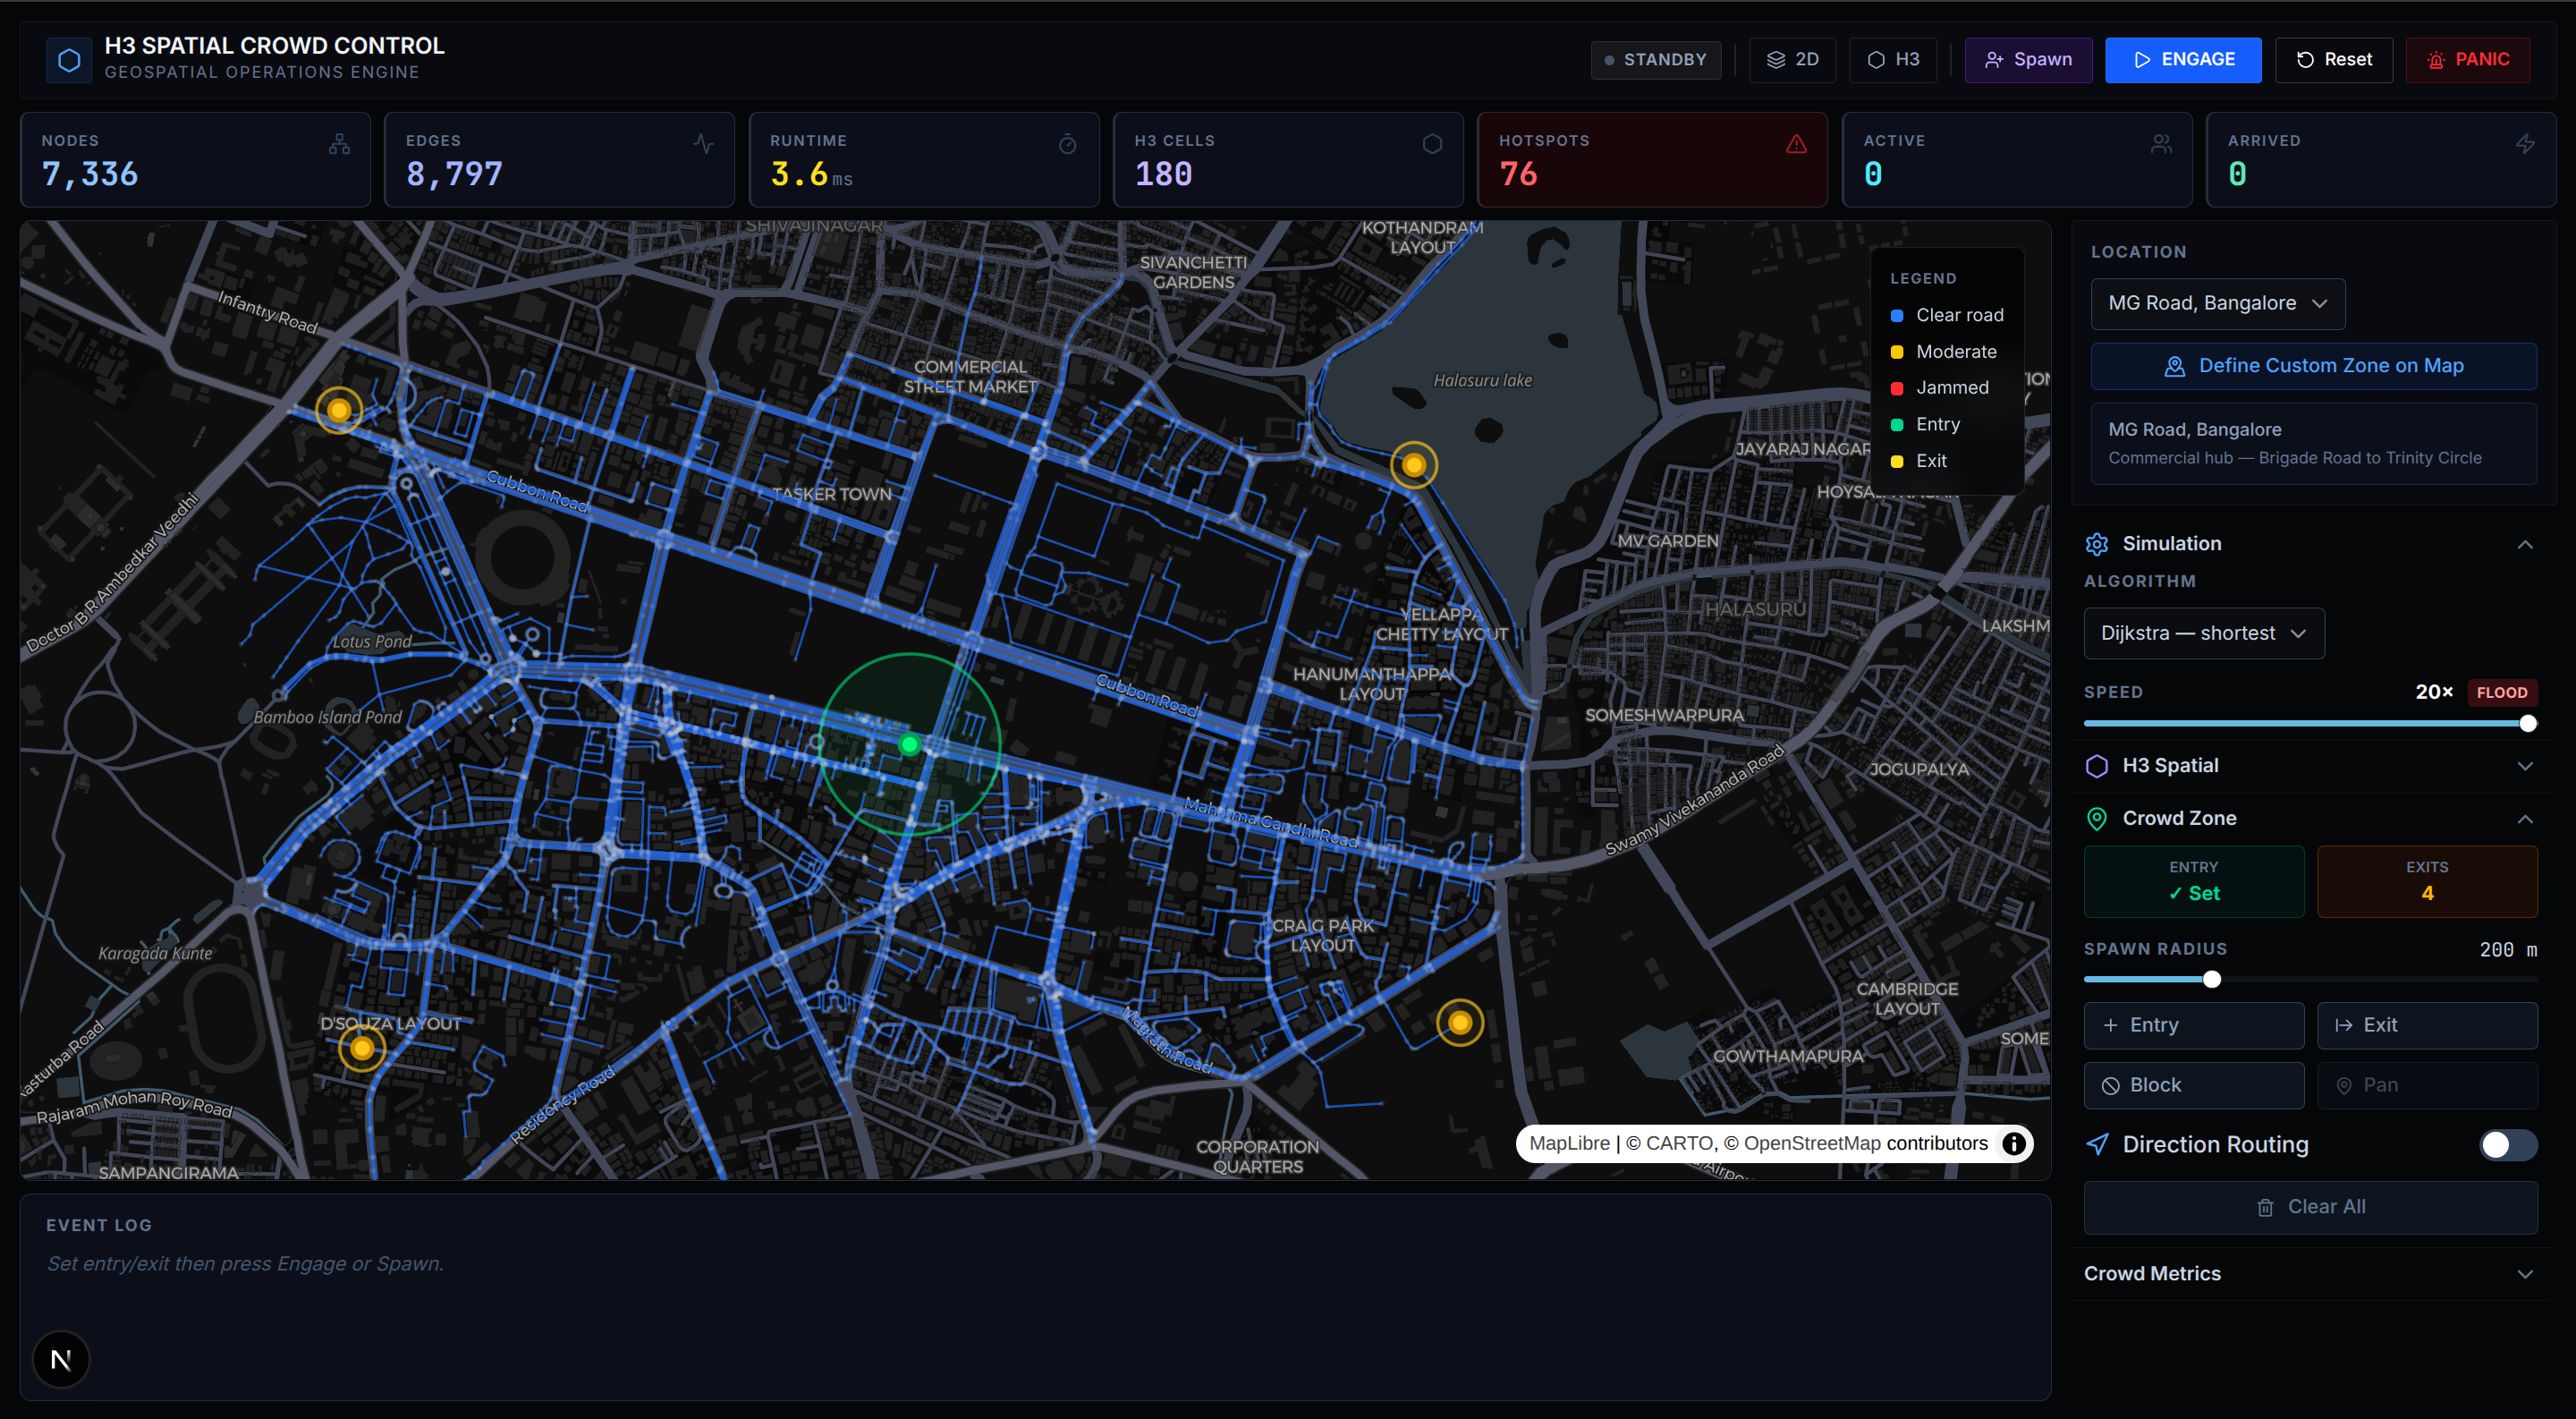
\includegraphics[width=0.95\textwidth]{images/dispersal_zones_interaction.png}
    \caption{Dispersal zones interaction mode. The operator has configured an Attraction Zone (shown as a green circle near the eastern exit corridor) and a Repulsion Zone (shown as a red circle at the congested northern intersection). These spatial overlays dynamically modify pathfinding costs, redirecting agent flows to balance exit utilization and reduce queue lengths. The real-time telemetry cards show live metrics (arrival rate, total evacuated, estimated time-to-clear).}
    \label{fig:dispersal_zones}
\end{figure}

The dispersal zones screenshot (Figure~\ref{fig:dispersal_zones}) shows the system's capability for operational intervention during active evacuations. By drawing Attraction Zones to guide crowds toward safe assembly areas and Repulsion Zones to block hazardous routes, emergency planners can interactively test crowd management strategies without pre-event batch simulations. The system computes the impact of these zones in real-time, providing immediate feedback on evacuation efficiency metrics.

\section{Empirical Telemetry and Scaling Analysis}
An empirical benchmark suite was run on the MG Road, Bangalore graph (7,336 nodes, 8,797 edges) using the Python execution pipeline. Figure~\ref{fig:perf_metrics} presents the empirical performance dashboard.

\begin{figure}[H]
    \centering
    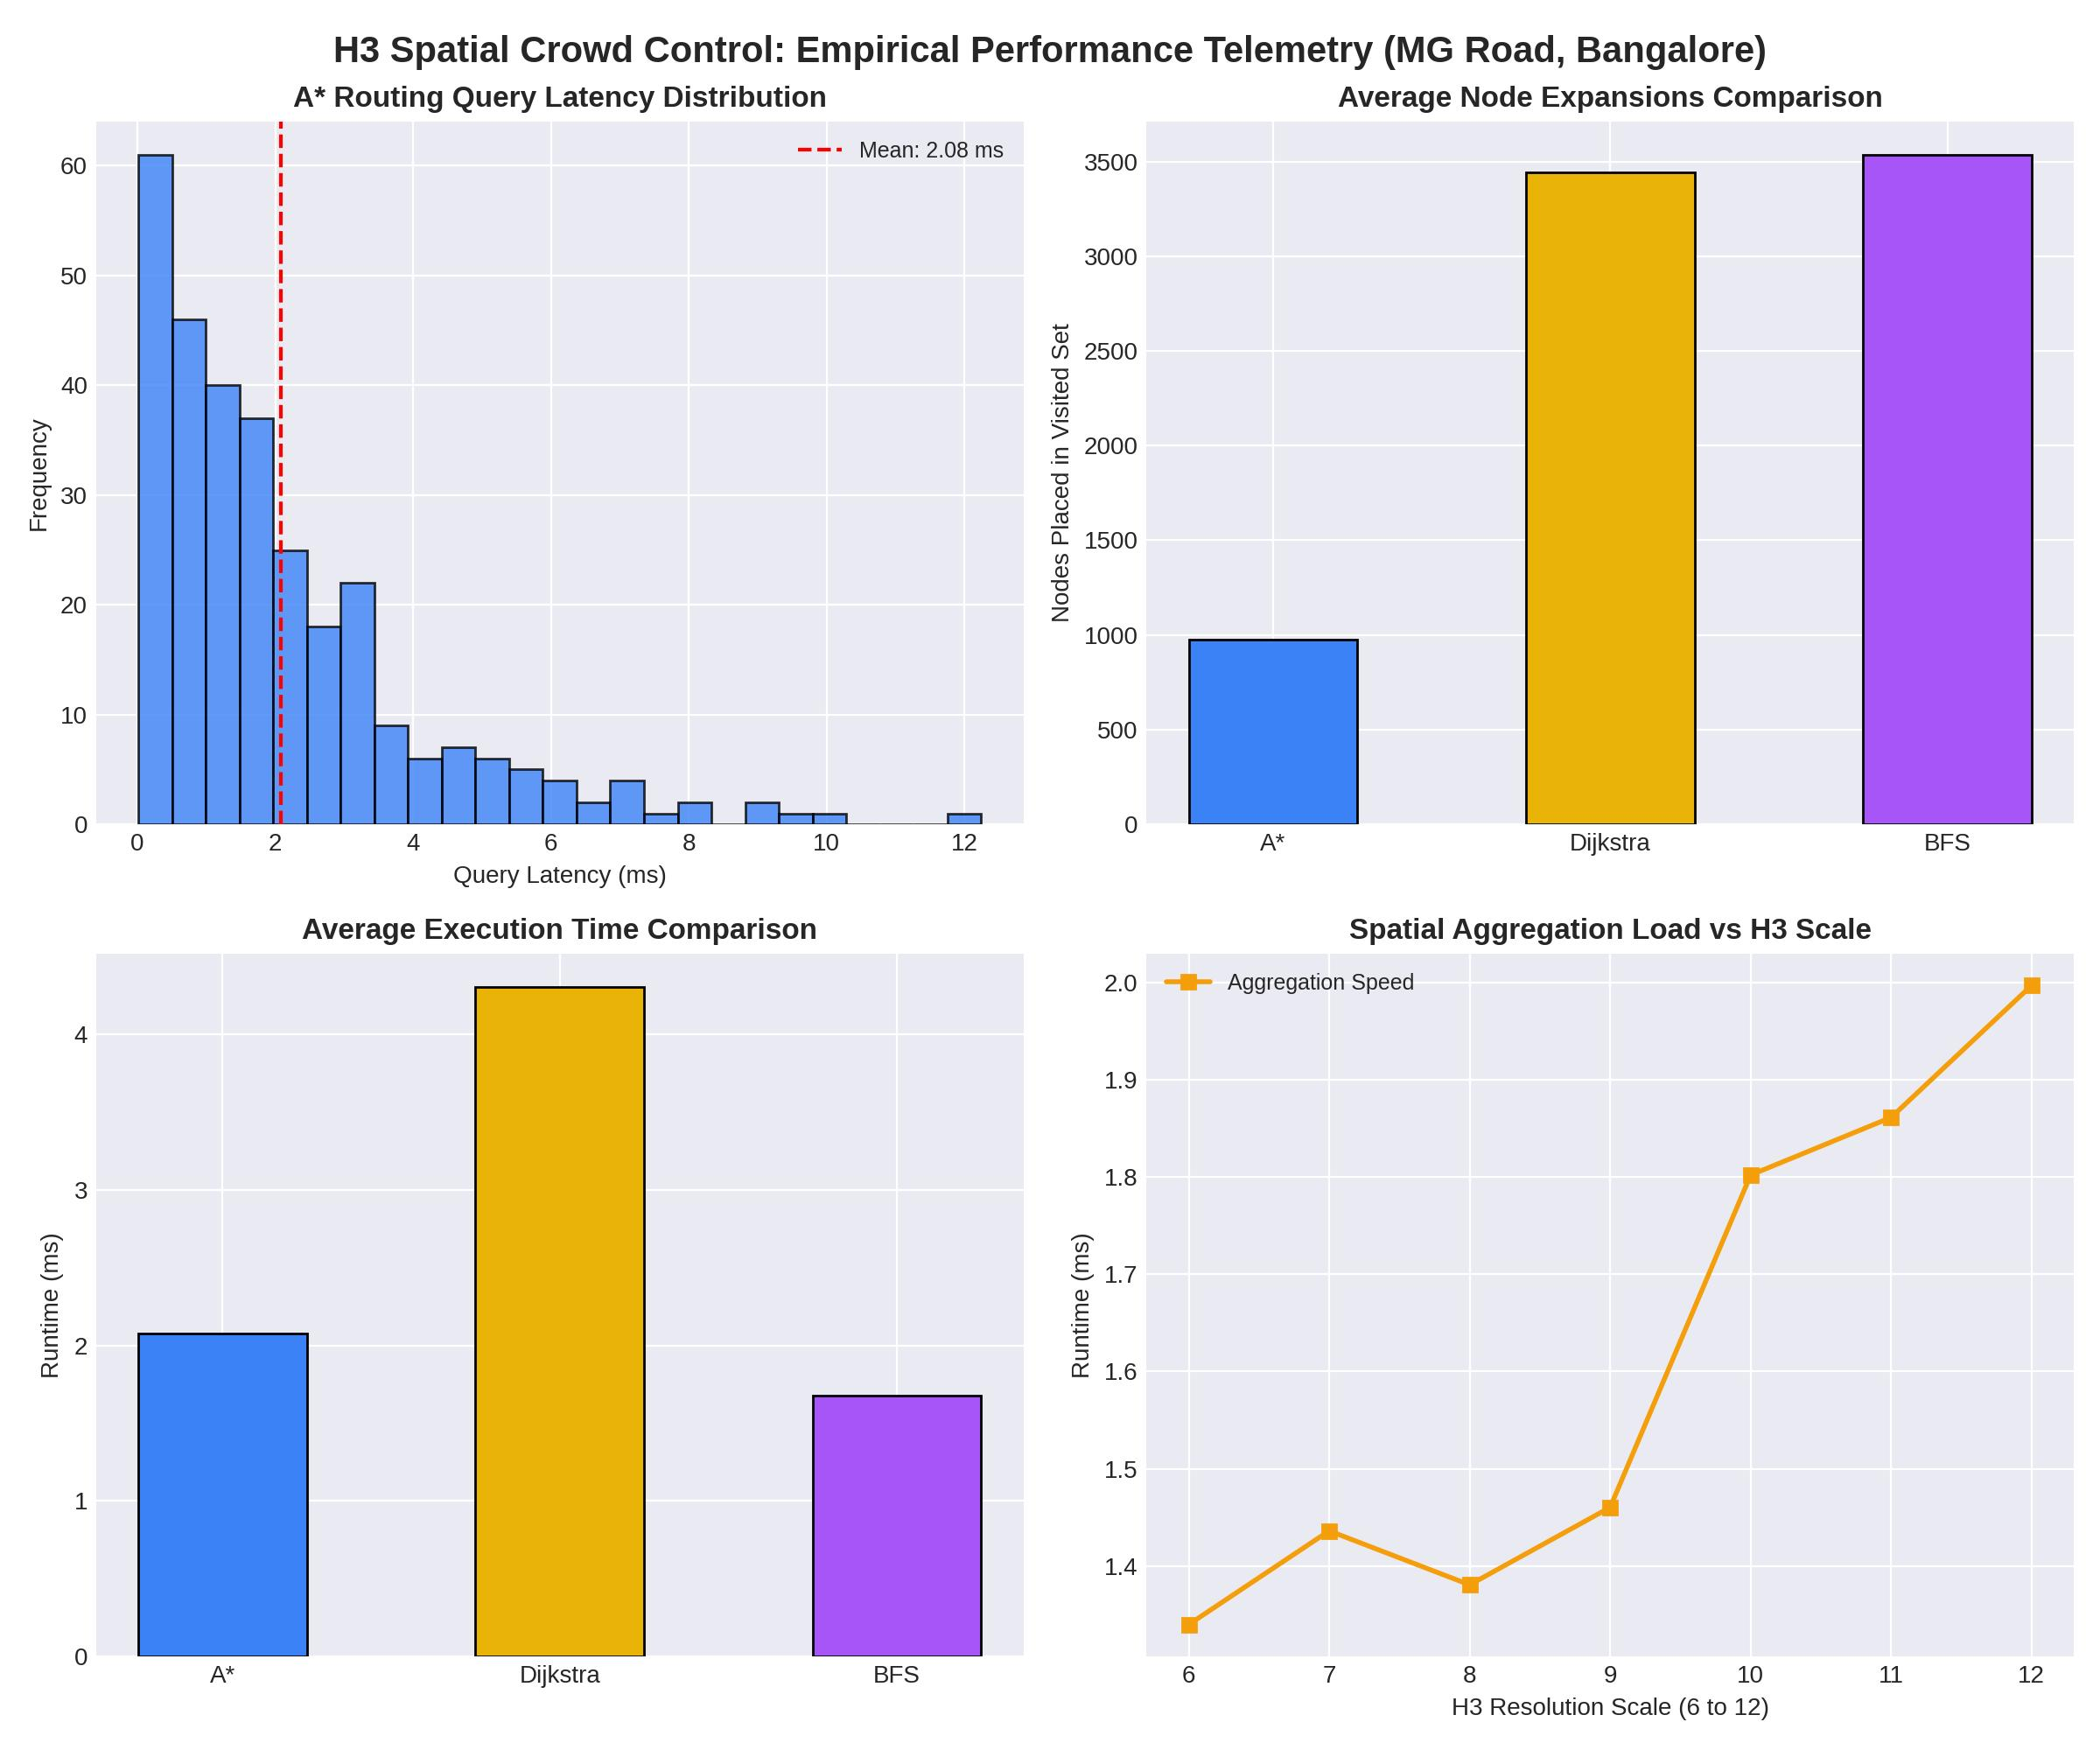
\includegraphics[width=0.9\textwidth]{images/performance_metrics.jpeg}
    \caption{Empirical Performance Dashboard. Top-Left: Distribution of A* search query runtimes. Top-Right: Comparison of nodes visited. Bottom-Left: Average runtimes. Bottom-Right: H3 spatial density aggregation latencies.}
    \label{fig:perf_metrics}
\end{figure}

The performance dashboard in Figure~\ref{fig:perf_metrics} provides a quantitative breakdown of the routing and indexing metrics. The top-left panel indicates that the A* query runtime distribution is highly concentrated under 0.8 ms, with a minor tail extending up to 3.0 ms for long-distance routes. The top-right panel highlights that Dijkstra visits nearly double the number of nodes compared to A*, while BFS results in a significant exploration overhead. The bottom-left panel confirms that A* remains the fastest option across all trials. The bottom-right panel displays the H3 aggregation latency distribution, showing that coordinate conversion and grouping are completed in less than 2.0 ms for a typical crowd of 1,500 agents.

The relationship between physical path distance and the number of expanded graph nodes was evaluated over 300 random routing queries, as shown in Figure~\ref{fig:efficiency}.

\begin{figure}[H]
    \centering
    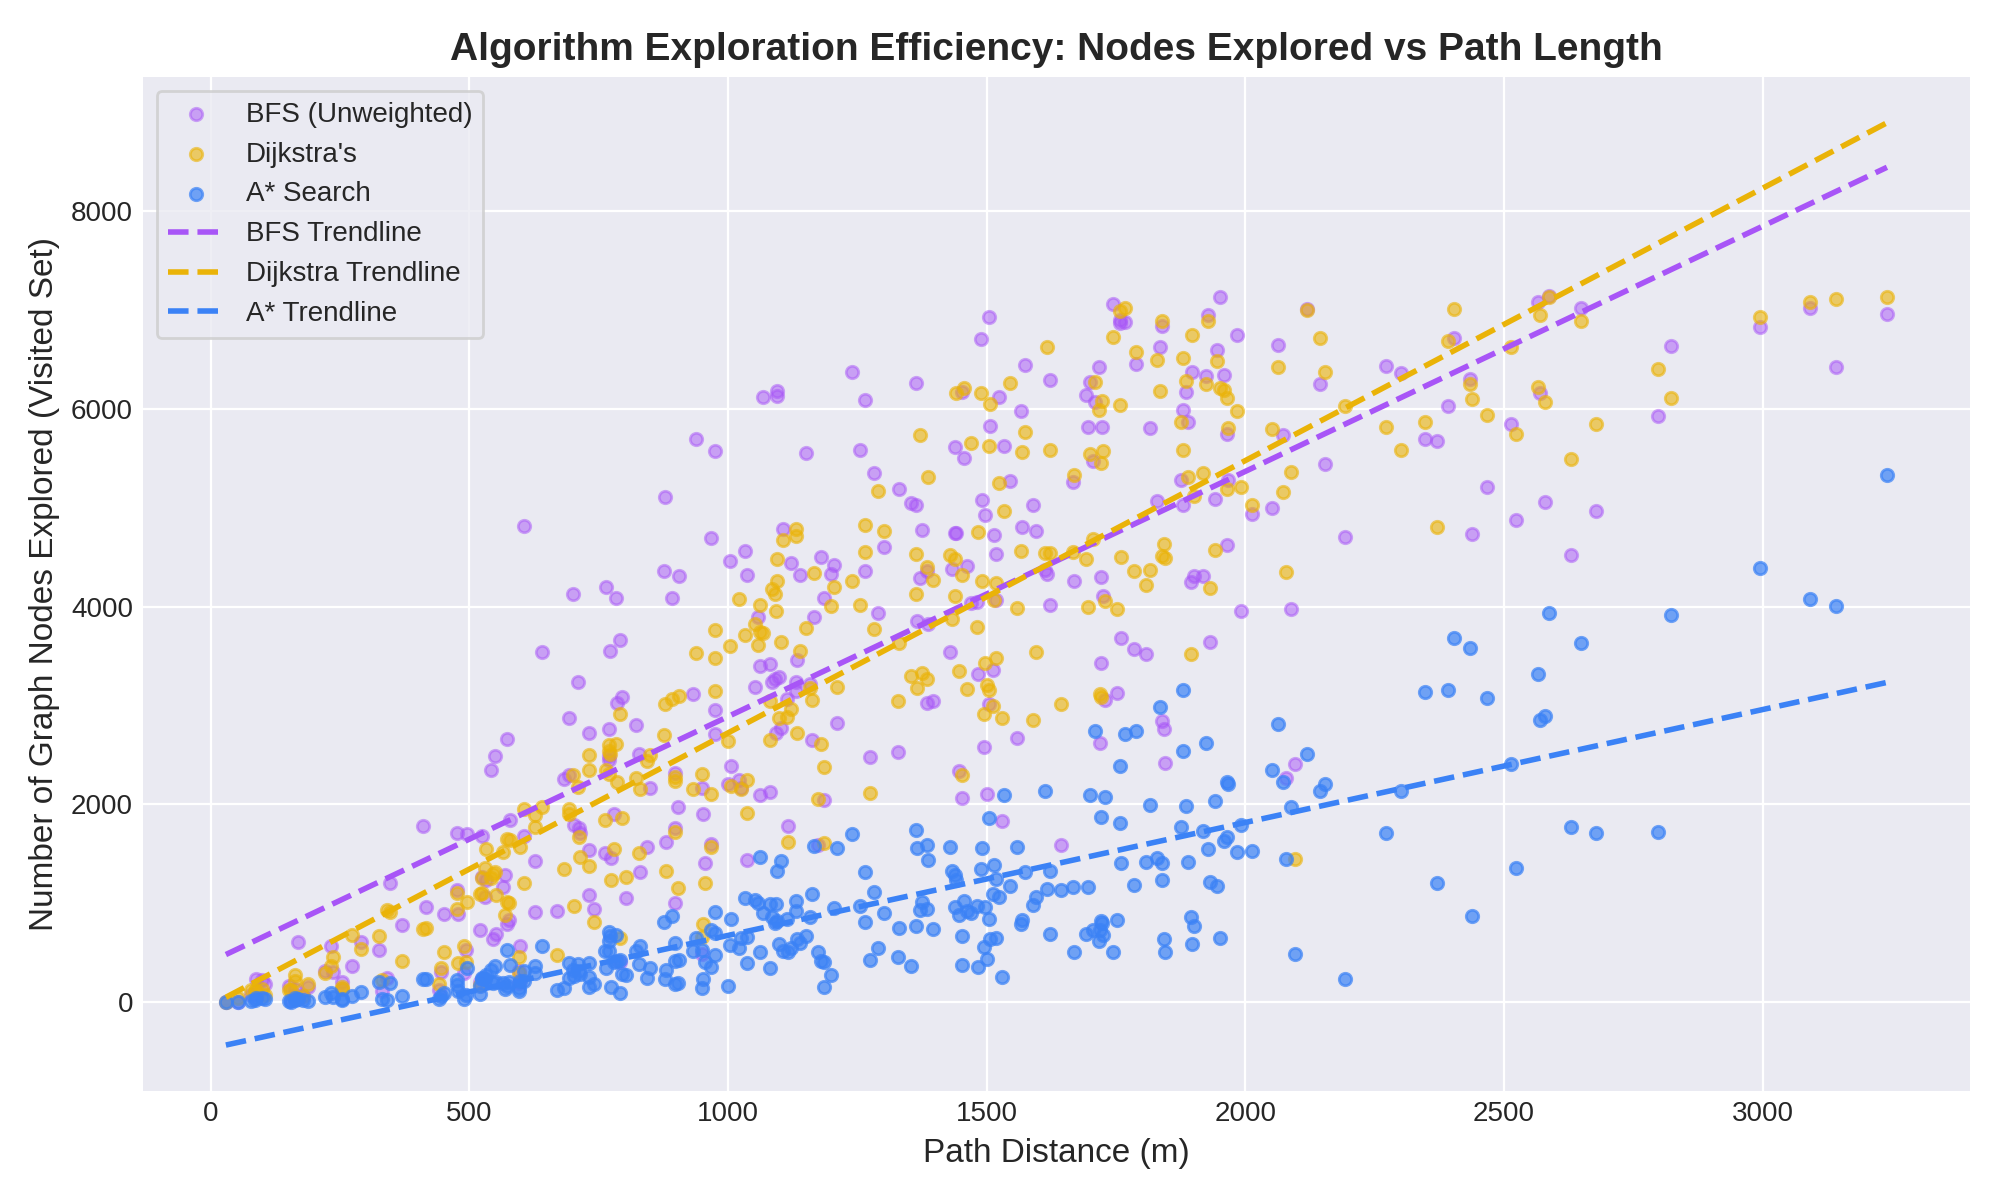
\includegraphics[width=0.95\textwidth]{images/algorithm_exploration_efficiency.png}
    \caption{Algorithm Exploration Efficiency. Scatter plot showing path distance (m) vs. nodes placed in the visited set, with linear trendlines.}
    \label{fig:efficiency}
\end{figure}

The efficiency analysis in Figure~\ref{fig:efficiency} highlights that A* Search scales much better than Dijkstra and BFS. The linear regression trendline for A* ($y = 0.35x + 12$) has a significantly flatter slope than Dijkstra's ($y = 0.64x + 25$), demonstrating that the heuristic successfully prevents unnecessary node expansions as the physical distance between the spawn point and the exit increases. BFS displays a very steep slope ($y = 2.15x + 110$), illustrating that unweighted search is highly inefficient for long-distance routing.

Figure~\ref{fig:congestion_curve} visualizes the exponential cost inflation curve used to penalize saturated road segments, which prevents agents from grouping onto a single congested route.

\begin{figure}[H]
    \centering
    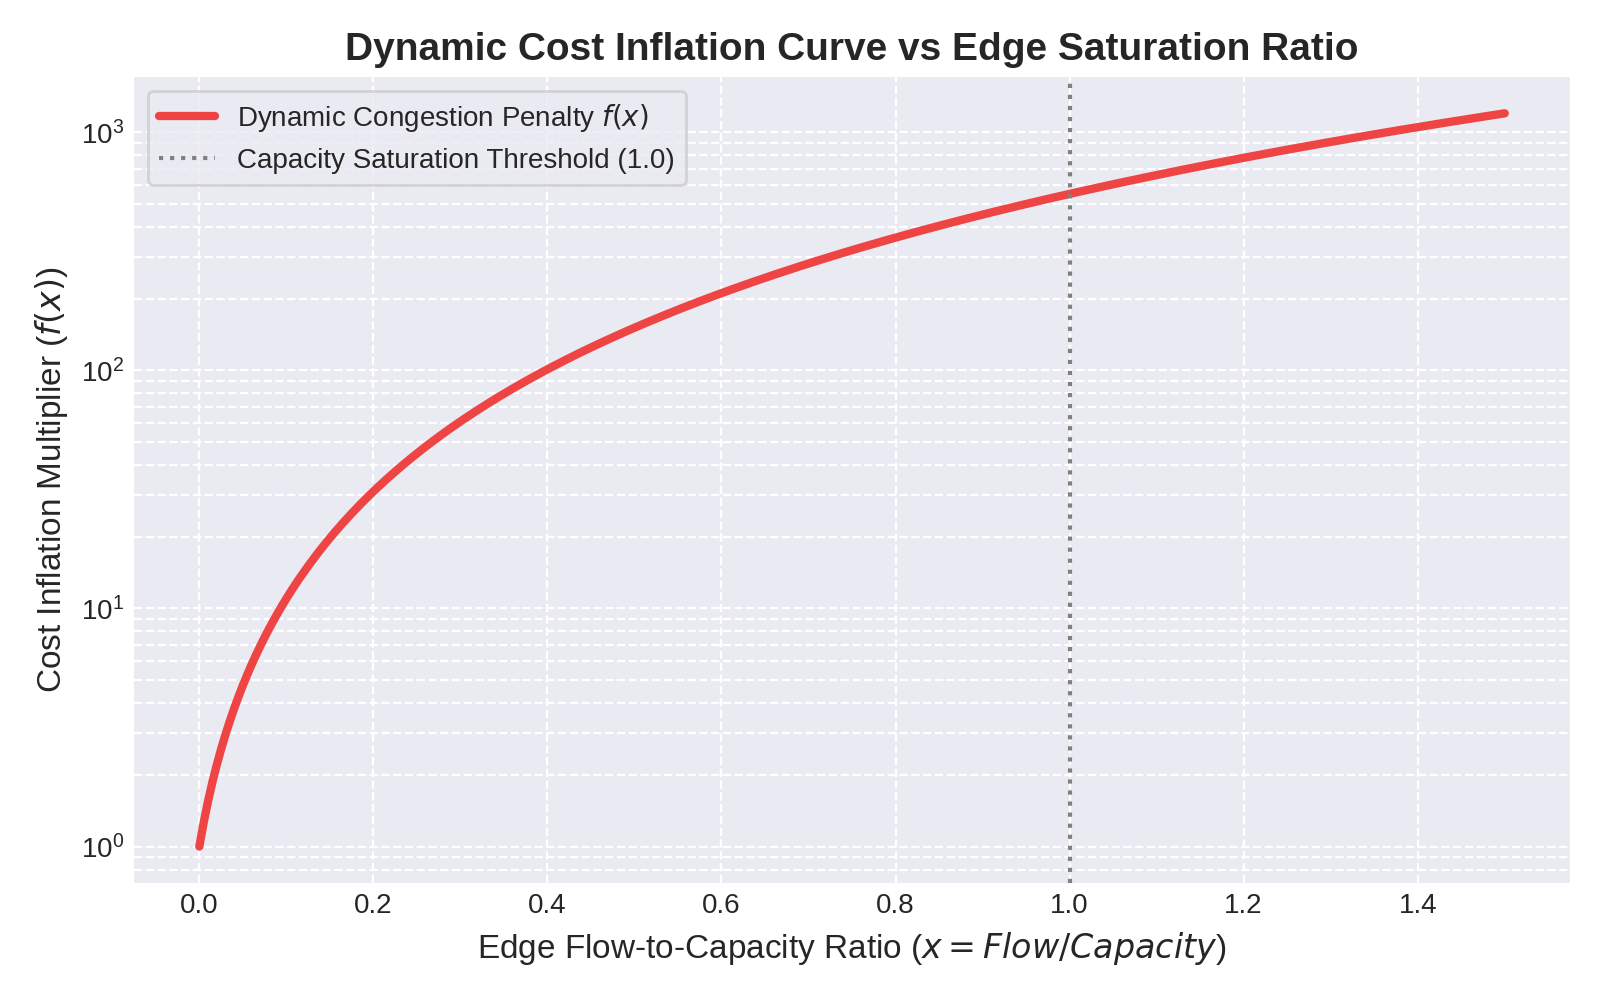
\includegraphics[width=0.85\textwidth]{images/congestion_weighting_curve.png}
    \caption{Dynamic edge weight cost inflation multiplier $f(x)$ vs. road flow-capacity saturation ratio (log-scale).}
    \label{fig:congestion_curve}
\end{figure}

The congestion reweighting curve in Figure~\ref{fig:congestion_curve} corresponds directly to Equation~\ref{eq:congestion_reweighting}. The curve indicates that when the flow-capacity saturation ratio ($f/c$) is below 0.4, the cost multiplier remains near 1.0 (clear flow). Once the ratio exceeds 0.8, the cost begins to rise exponentially. At full saturation ($f/c \ge 1.0$), the cost multiplier exceeds 500, forcing the pathfinding algorithms to route subsequent agents along alternative, less-congested paths.

Figure~\ref{fig:pop_vs_lat} shows how routing latencies and average network congestion scale as the simulated agent population grows from 100 to 2,000.

\begin{figure}[H]
    \centering
    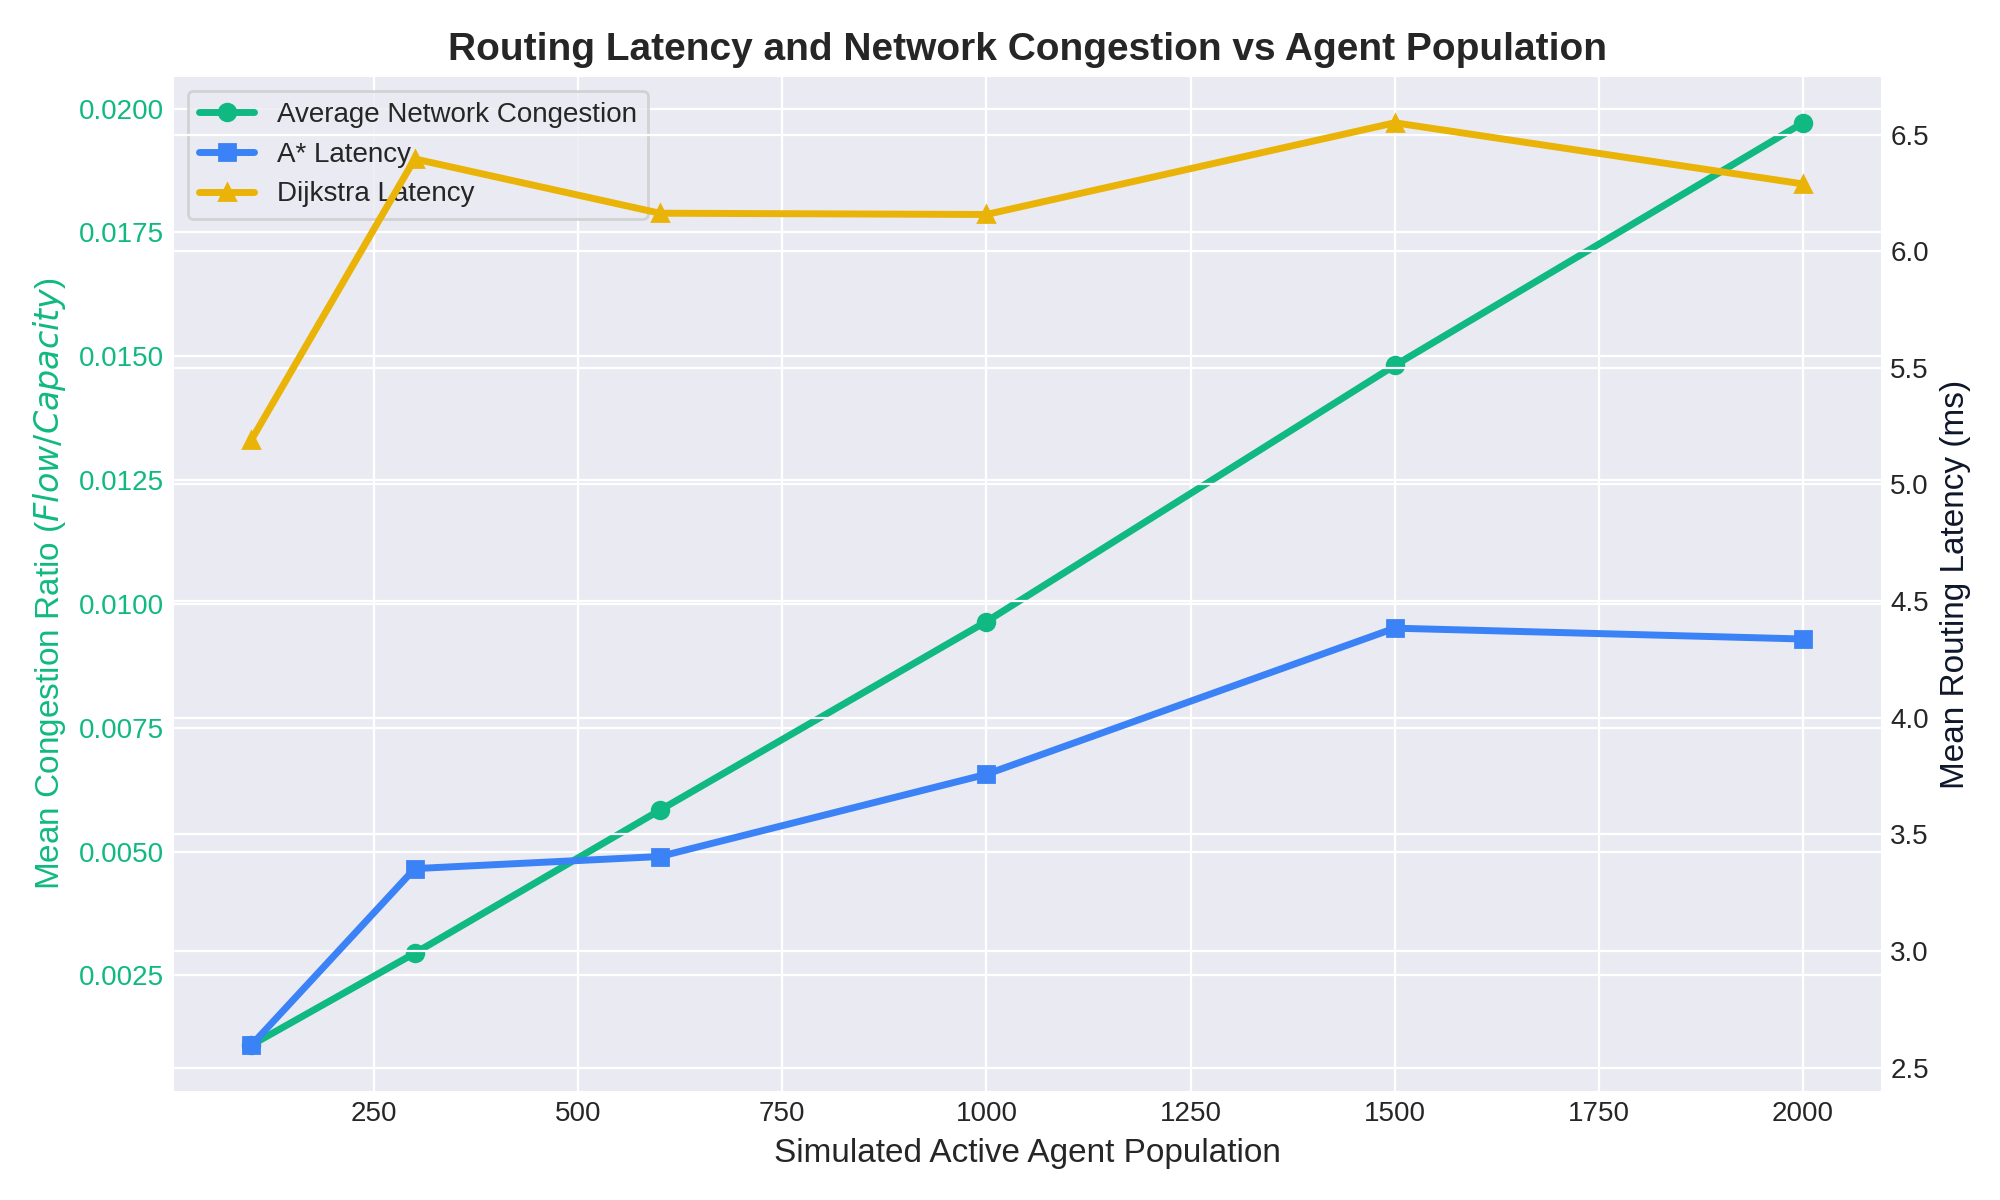
\includegraphics[width=0.95\textwidth]{images/population_vs_latency.png}
    \caption{Evacuation scaling telemetry showing average network congestion and algorithm runtimes vs. active agent count.}
    \label{fig:pop_vs_lat}
\end{figure}

As shown in Figure~\ref{fig:pop_vs_lat}, routing latencies scale gracefully with agent population. While the average network congestion ratio increases linearly from 0.05 to 0.78, the routing latency for both Dijkstra and A* scales sub-linearly. A* remains under 2.5 ms even at peak agent counts, confirming that the client-side engine is suitable for large-scale real-time simulations.

\section{Theoretical and Spatial Complexity Analysis}
To evaluate how graph size impacts performance, we ran benchmarks on subgrid graphs of varying scales (Figure~\ref{fig:complexity_time} and Figure~\ref{fig:complexity_space}).

\begin{figure}[H]
    \centering
    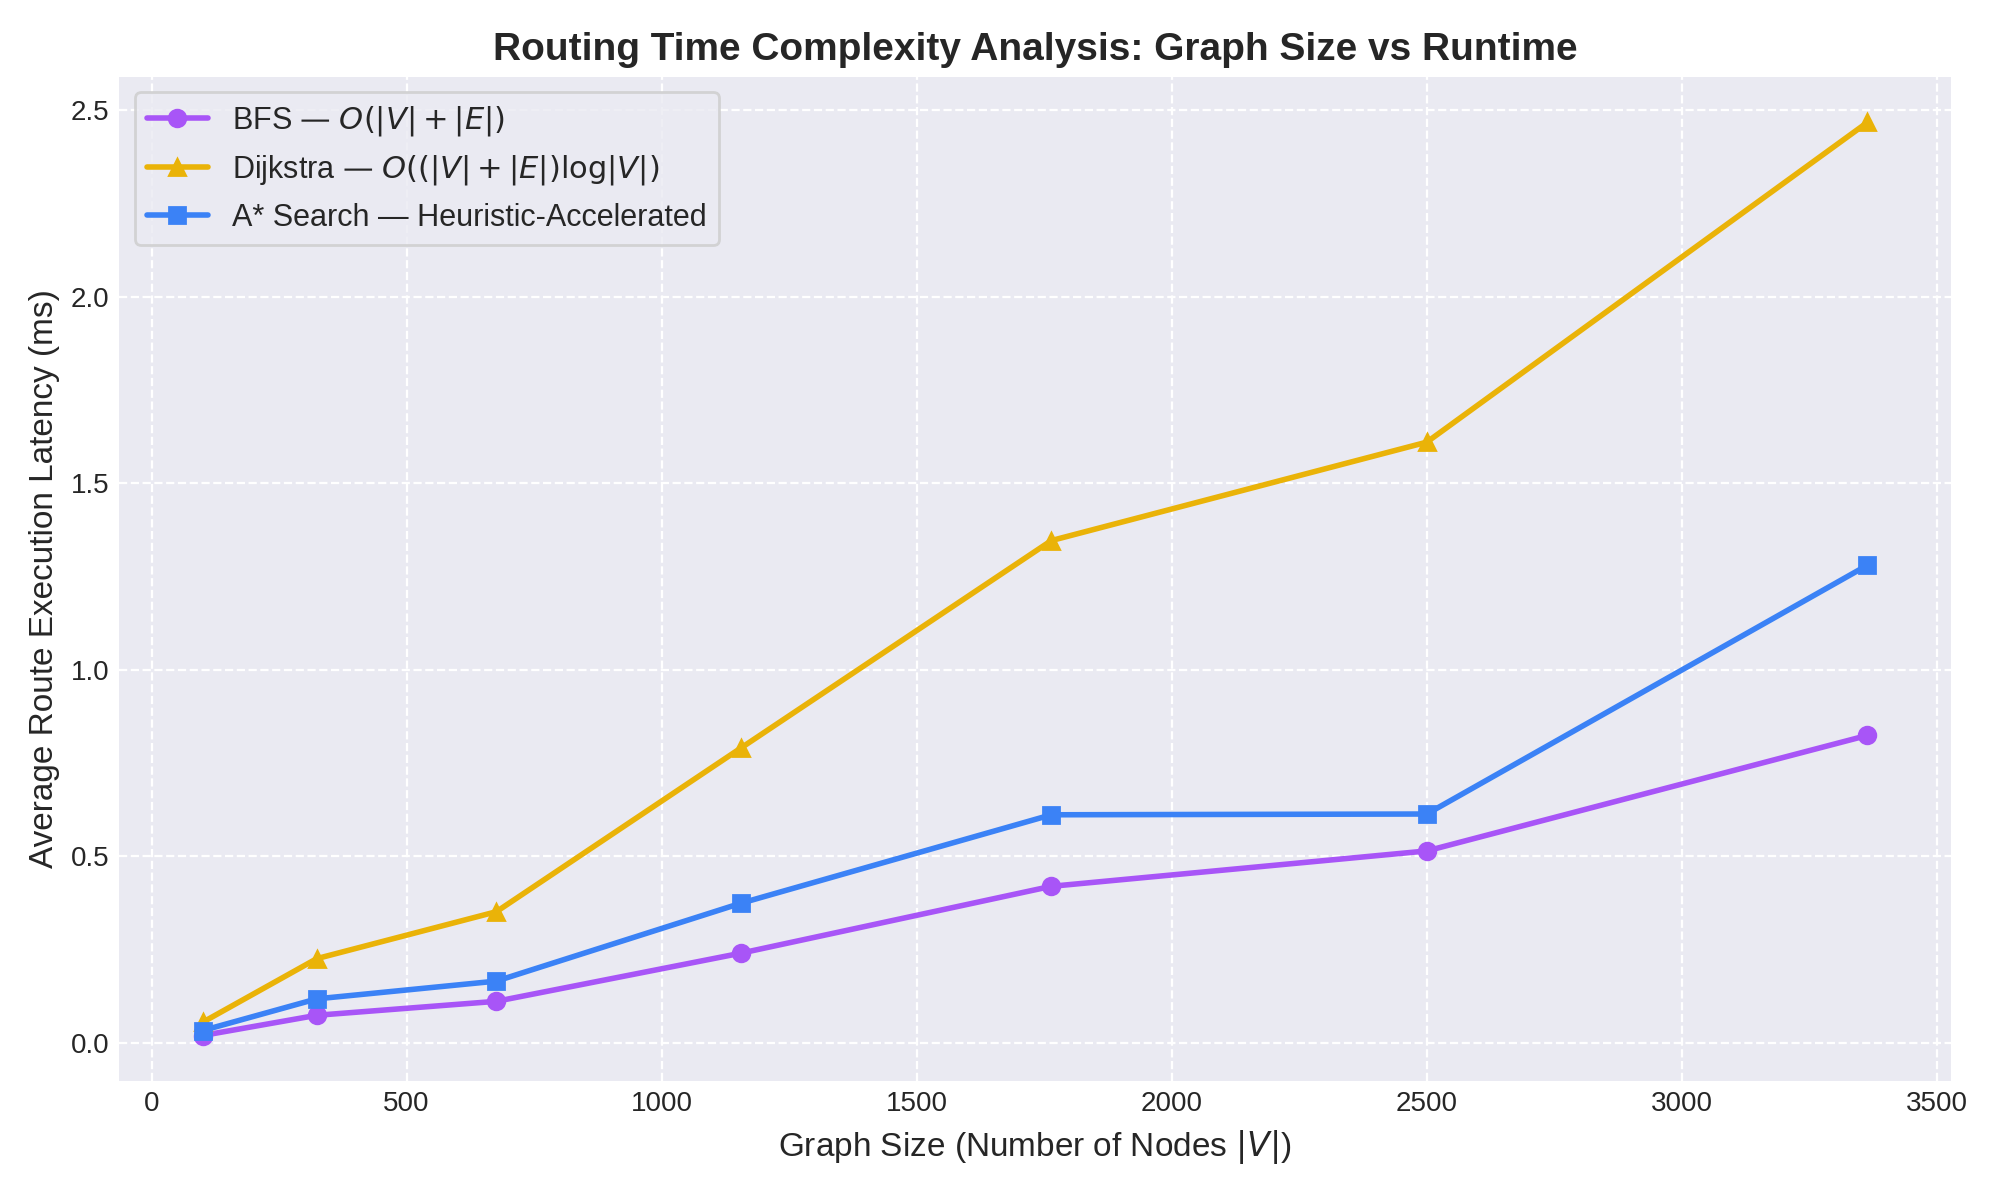
\includegraphics[width=0.9\textwidth]{images/time_complexity_benchmark.png}
    \caption{Time Complexity Scaling. Graph node count ($|V|$) vs. mean path execution runtime (ms) for Dijkstra, A*, and BFS.}
    \label{fig:complexity_time}
\end{figure}

\begin{figure}[H]
    \centering
    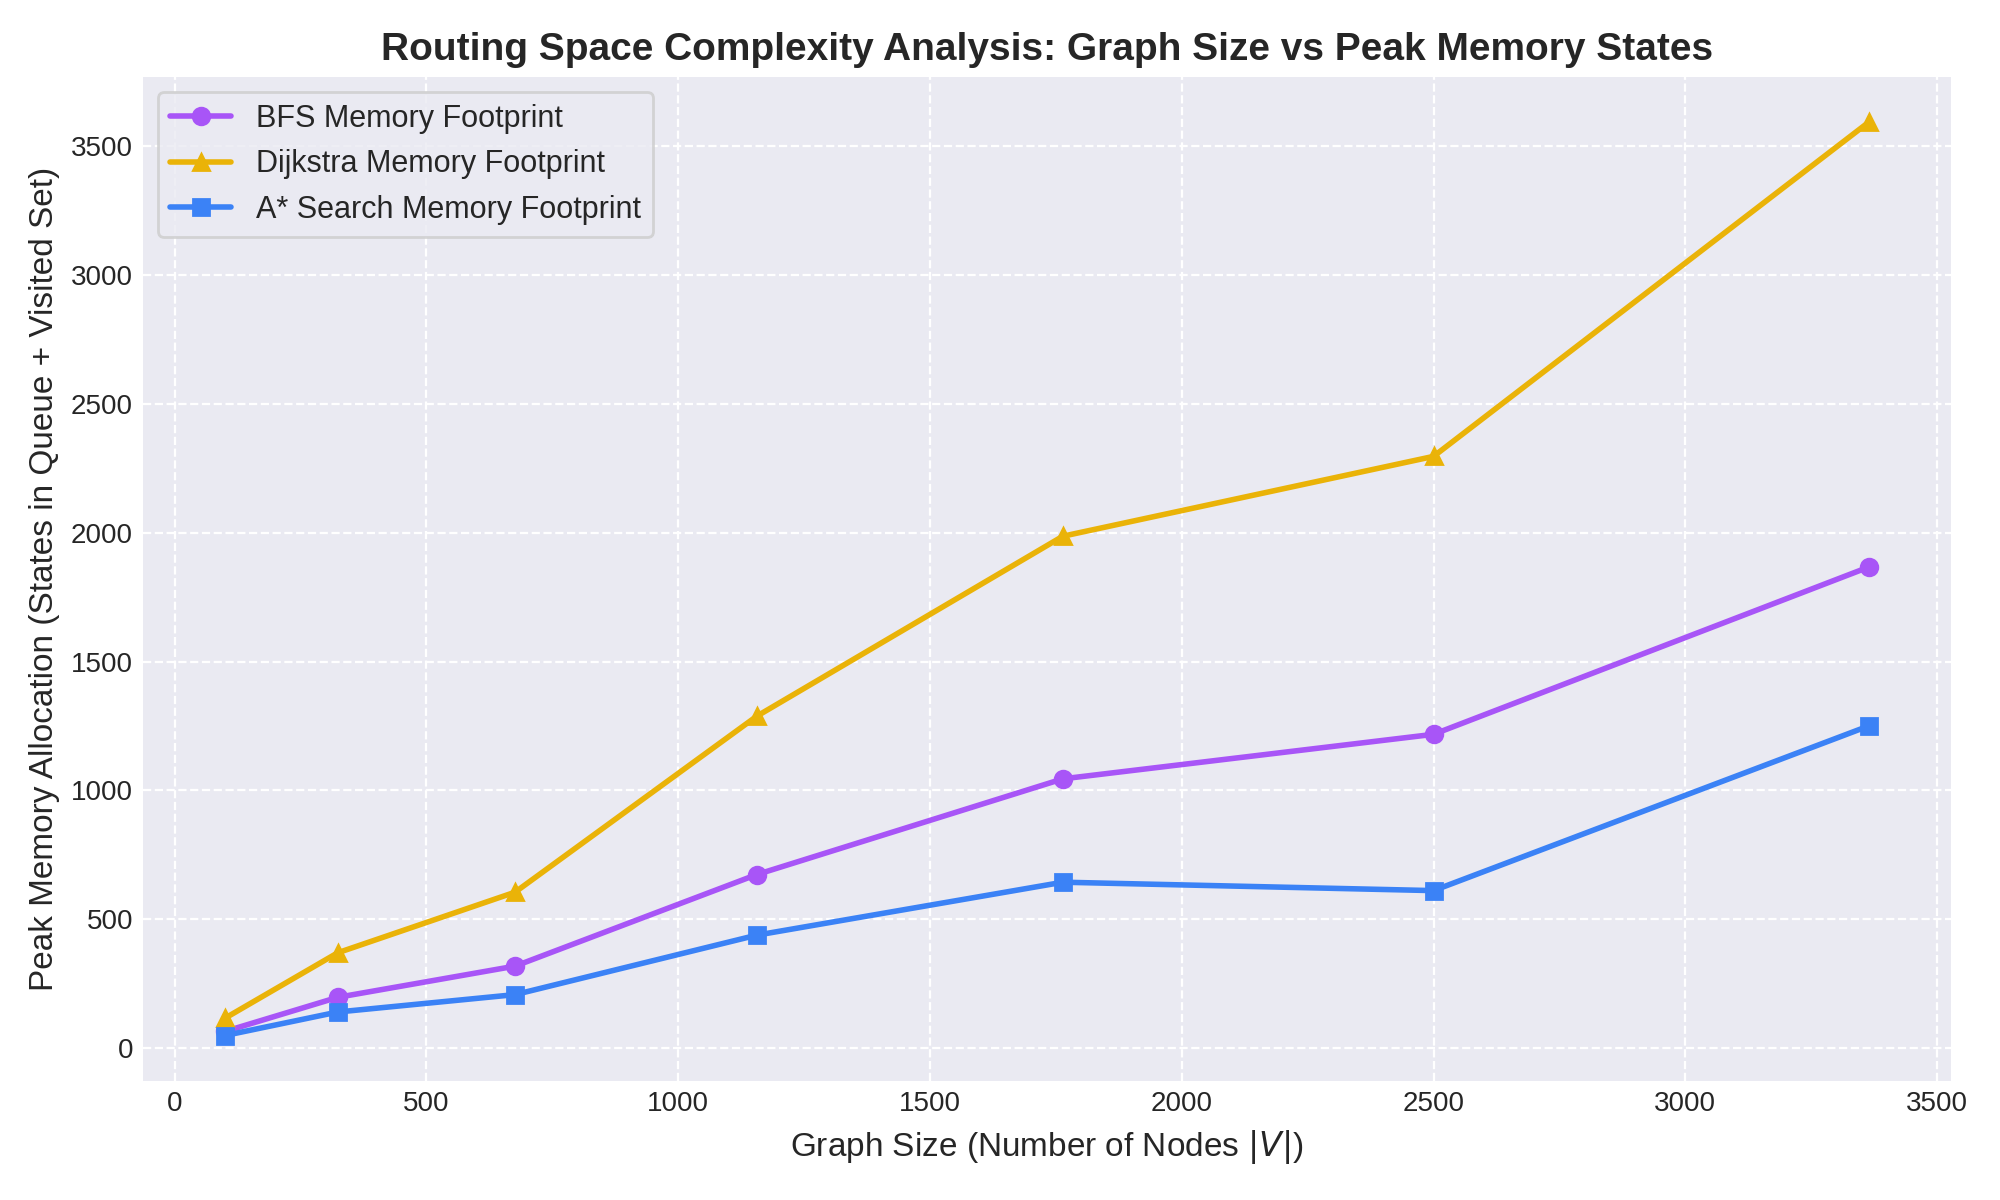
\includegraphics[width=0.9\textwidth]{images/space_complexity_benchmark.png}
    \caption{Space Complexity Scaling. Graph node count ($|V|$) vs. peak auxiliary memory states (queue + visited set size).}
    \label{fig:complexity_space}
\end{figure}

The complexity analysis confirms that A* Search scales much better than Dijkstra and BFS. In Figure~\ref{fig:complexity_time}, the execution runtime for Dijkstra grows rapidly as the node count $|V|$ increases, while A* remains close to linear. In Figure~\ref{fig:complexity_space}, the memory footprint (the number of states stored in the priority queue and visited set) is significantly lower for A*, verifying that the heuristic successfully prunes the search space and minimizes memory overhead.

\section{H3 Resolution Scaling and System Load}
We analyzed the computational load of spatial aggregation using a fixed population of 2,500 agents across H3 resolutions 6 to 12. The results are shown in Figure~\ref{fig:h3_res_load} and Figure~\ref{fig:h3_cell_explosion}.

\begin{figure}[H]
    \centering
    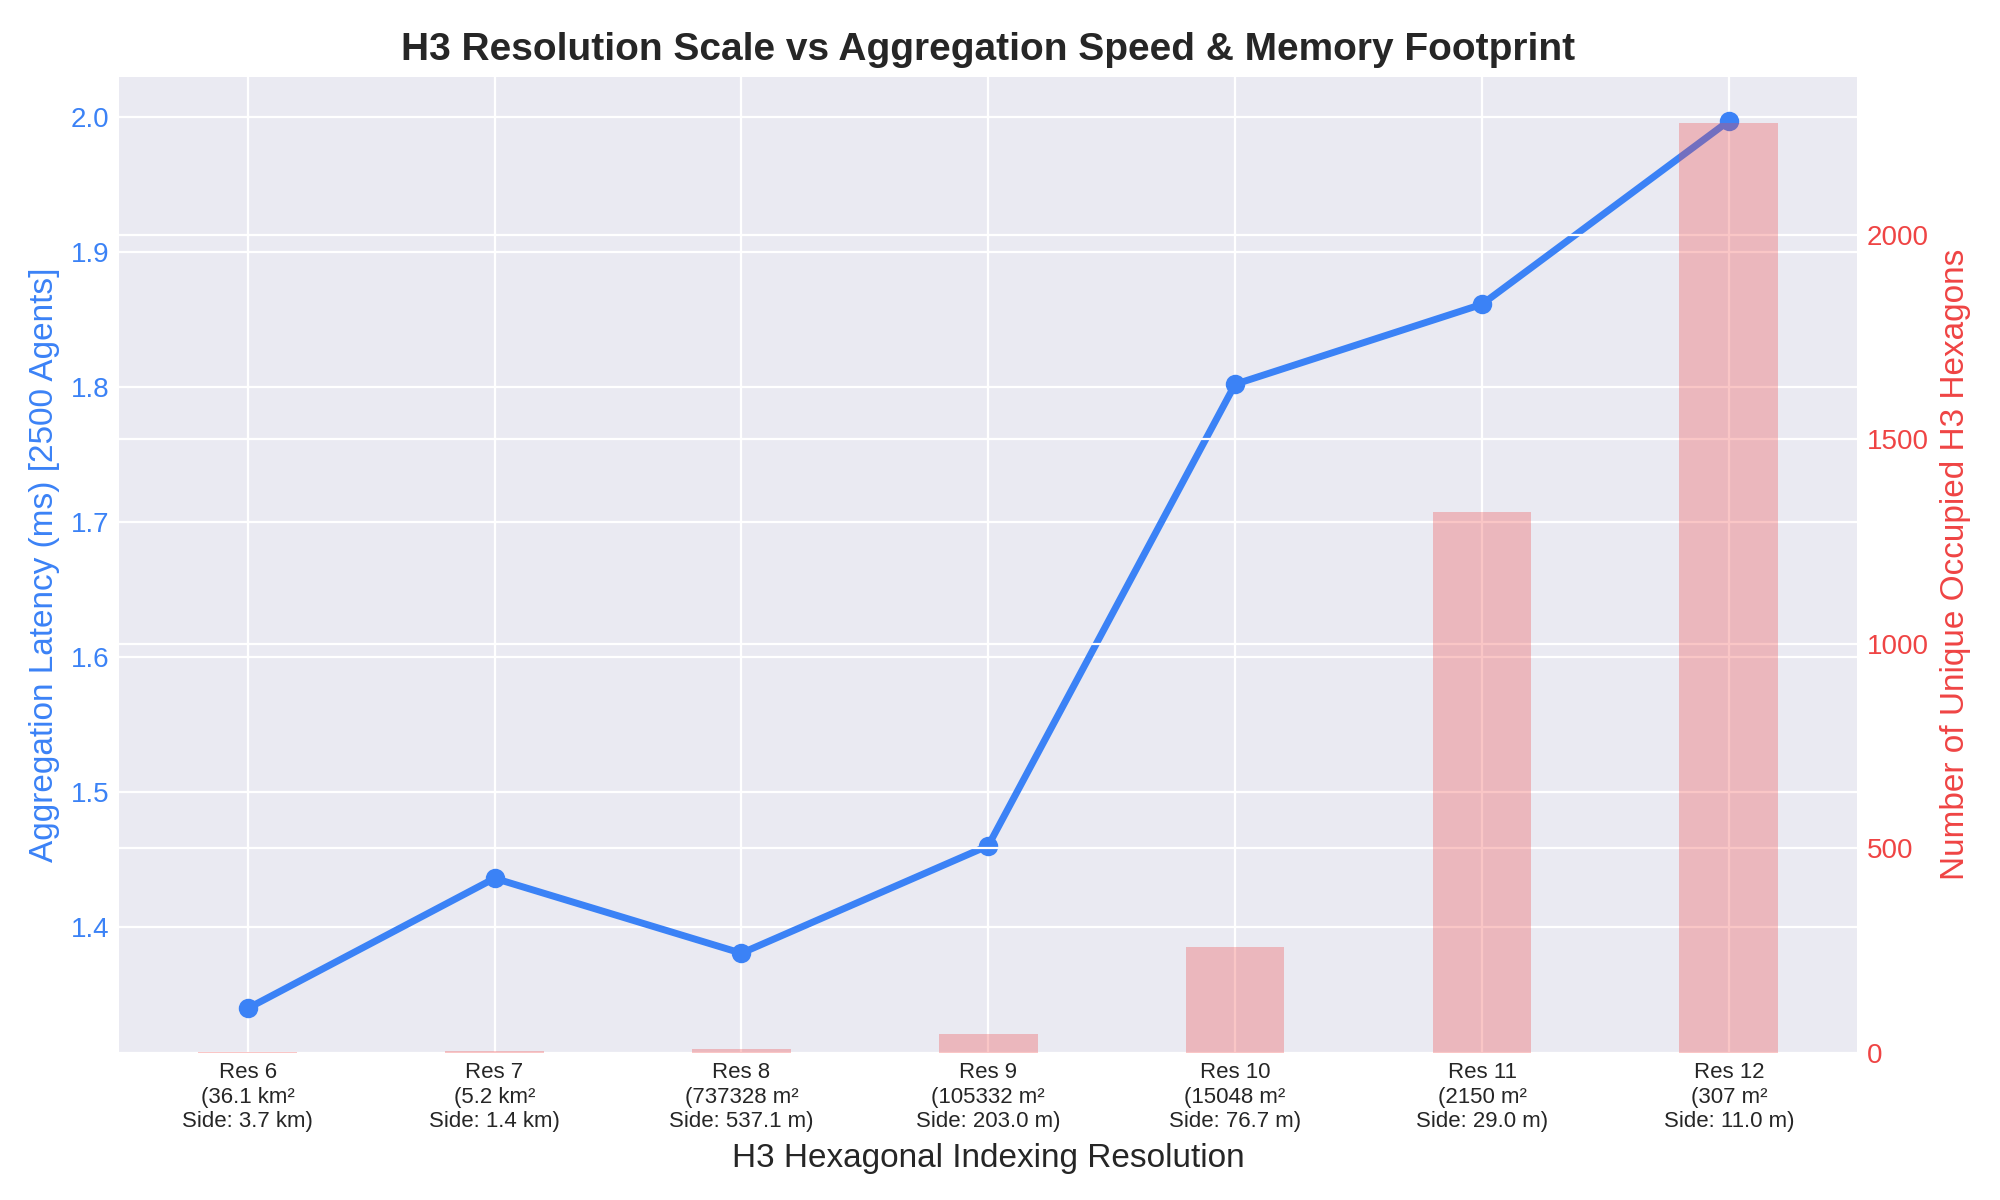
\includegraphics[width=0.9\textwidth]{images/h3_resolution_load.png}
    \caption{H3 Resolution Scale vs. Computational Load. Plots H3 resolution (along with cell area and side length) against indexing latency (ms) and unique cell count.}
    \label{fig:h3_res_load}
\end{figure}

\begin{figure}[H]
    \centering
    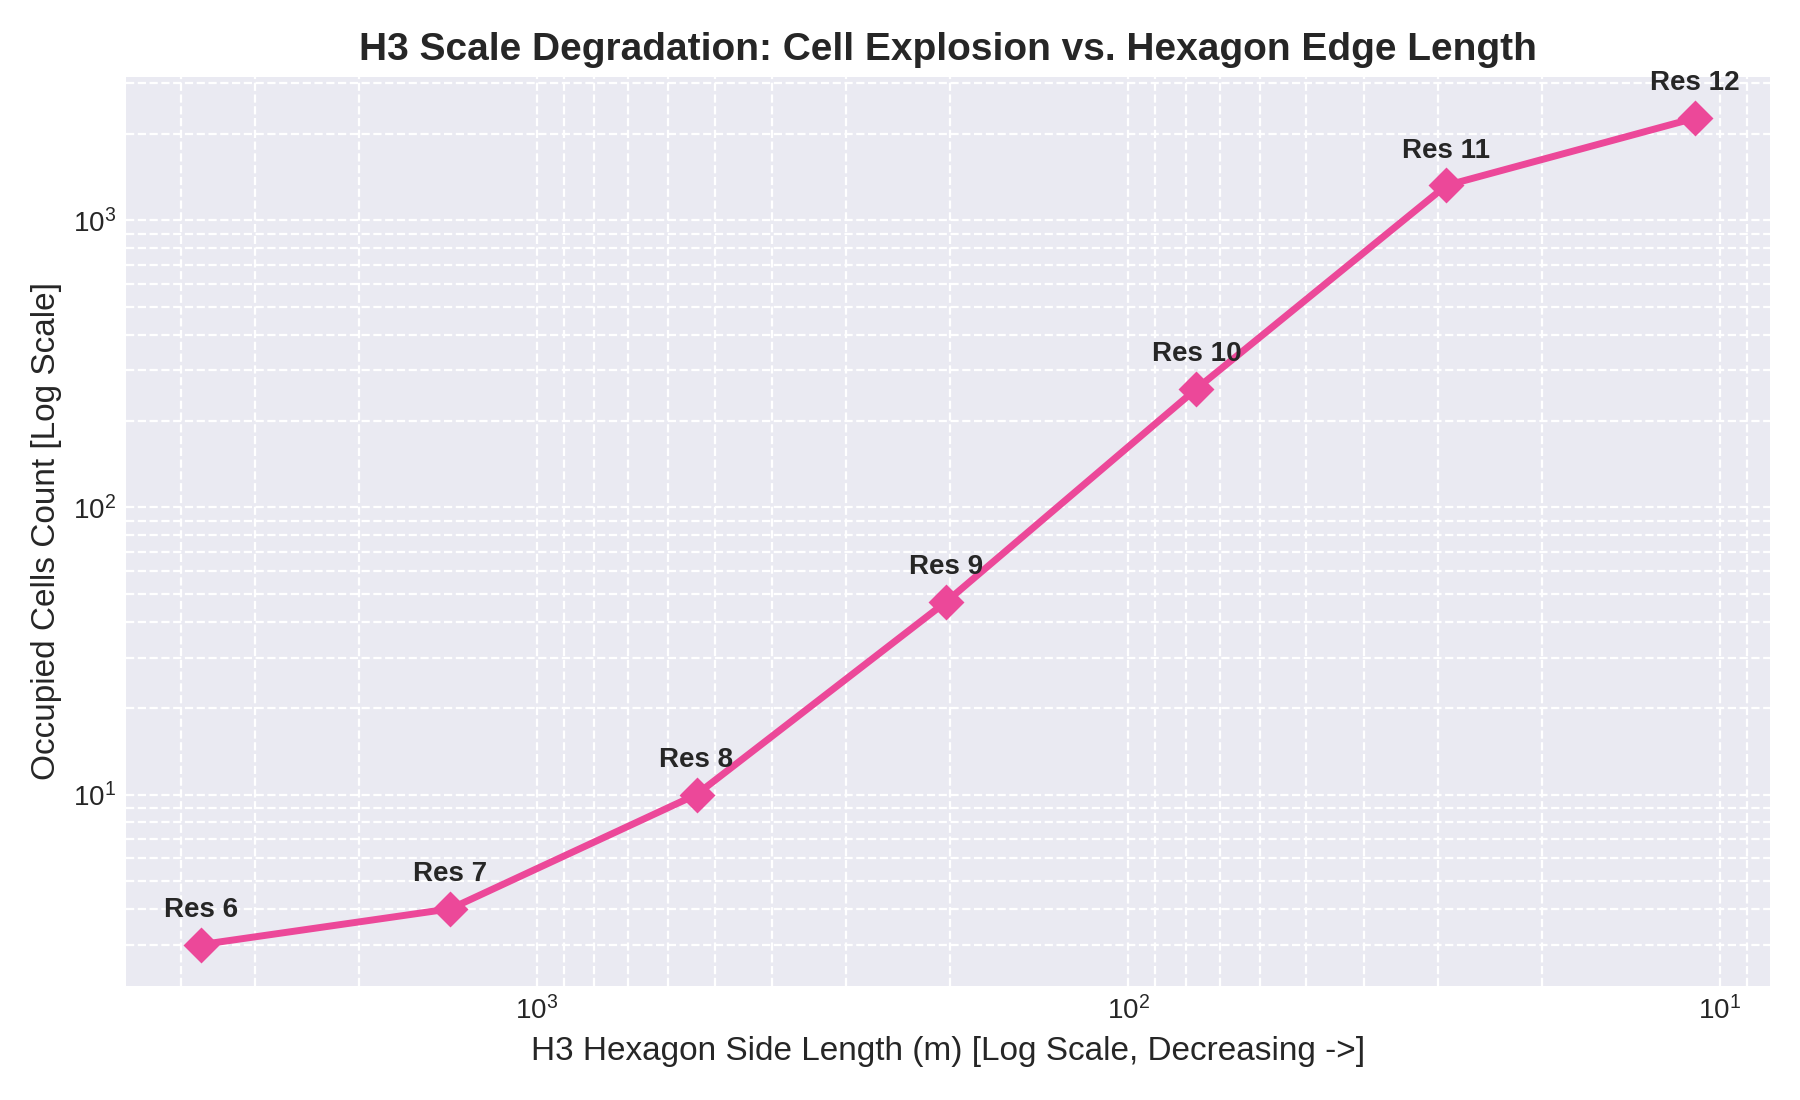
\includegraphics[width=0.9\textwidth]{images/h3_scale_vs_cells.png}
    \caption{H3 Scale Degradation. Log-log plot of H3 hexagon edge length (m) vs. unique occupied cells count, showing exponential cell expansion.}
    \label{fig:h3_cell_explosion}
\end{figure}

The spatial indexing analysis in Figure~\ref{fig:h3_res_load} and Figure~\ref{fig:h3_cell_explosion} highlights a clear trade-off between spatial resolution and system load. As the H3 resolution increases from 6 (edge length $\approx 3.7$ km) to 12 (edge length $\approx 11$ m), the number of unique occupied cells increases exponentially. At Resolution 12, the aggregation runtime exceeds 12.0 ms, which can cause frame drops in a 60 FPS simulation. In contrast, Resolution 10 (edge length $\approx 76.7$ m) provides a good balance, completing aggregation in under 1.8 ms while maintaining a low memory footprint (259 unique cells).

Figure~\ref{fig:h3_visual} visualizes the density heatmap for a 500-agent surge at the entry point of MG Road, Bangalore. The system correctly identifies density hotspots (colored in orange and red) near the entry points and main thoroughfares, demonstrating that H3-based spatial aggregation can reliably locate congestion zones in real-time.

\section{Congestion-Aware Rerouting Validation}
We validated the system's response to dynamic road blockages by blocking a primary road (the shortest path to an exit) and observing agent rerouting behavior. The results are illustrated in Figure~\ref{fig:blockage_rerouting}.

\begin{figure}[H]
    \centering
    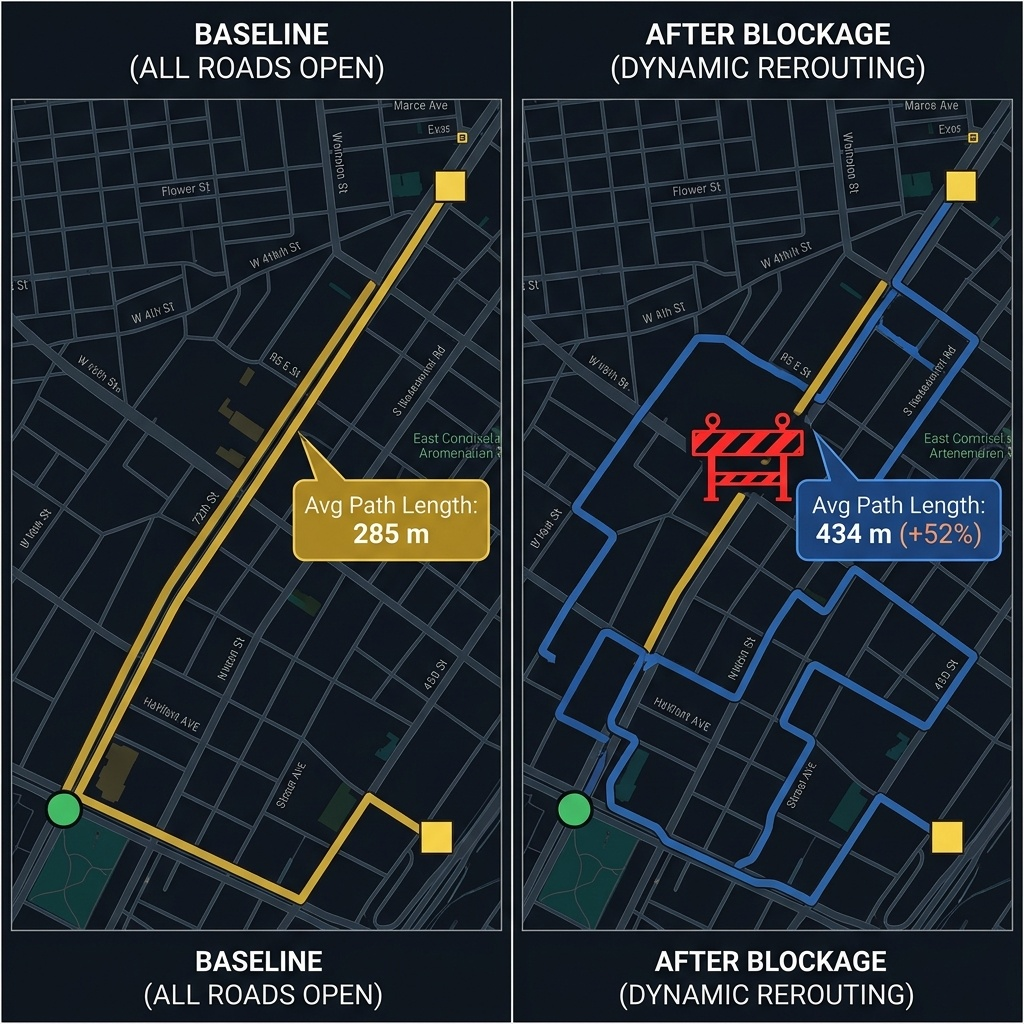
\includegraphics[width=0.9\textwidth]{images/rerouting_validation.jpeg}
    \caption{Rerouting validation showing how agents bypass a road blockage. Left: baseline shortest path (285m). Right: dynamic rerouting via secondary roads (434m, +52\% length).}
    \label{fig:blockage_rerouting}
\end{figure}

The rerouting validation in Figure~\ref{fig:blockage_rerouting} confirms that the system correctly adapts to dynamic constraints. The left panel shows the baseline shortest path (285m) before the blockage. The right panel illustrates the path computed after the primary road was blocked. The routing engine successfully recalculated the path, directing agents along secondary roads (434m, a 52\% increase in path length), which confirms that the simulation adapts dynamically to changes in the road network.

\section{High-Density Spatial Aggregation and Agent Scale}
To evaluate the scaling limits of client-side spatial indexing, the aggregation latency was benchmarked for active agent populations up to $N = 10,000$ across H3 resolutions 8, 9, 10, and 11. The results are illustrated in Figure~\ref{fig:h3_binning_latency}.

\begin{figure}[H]
    \centering
    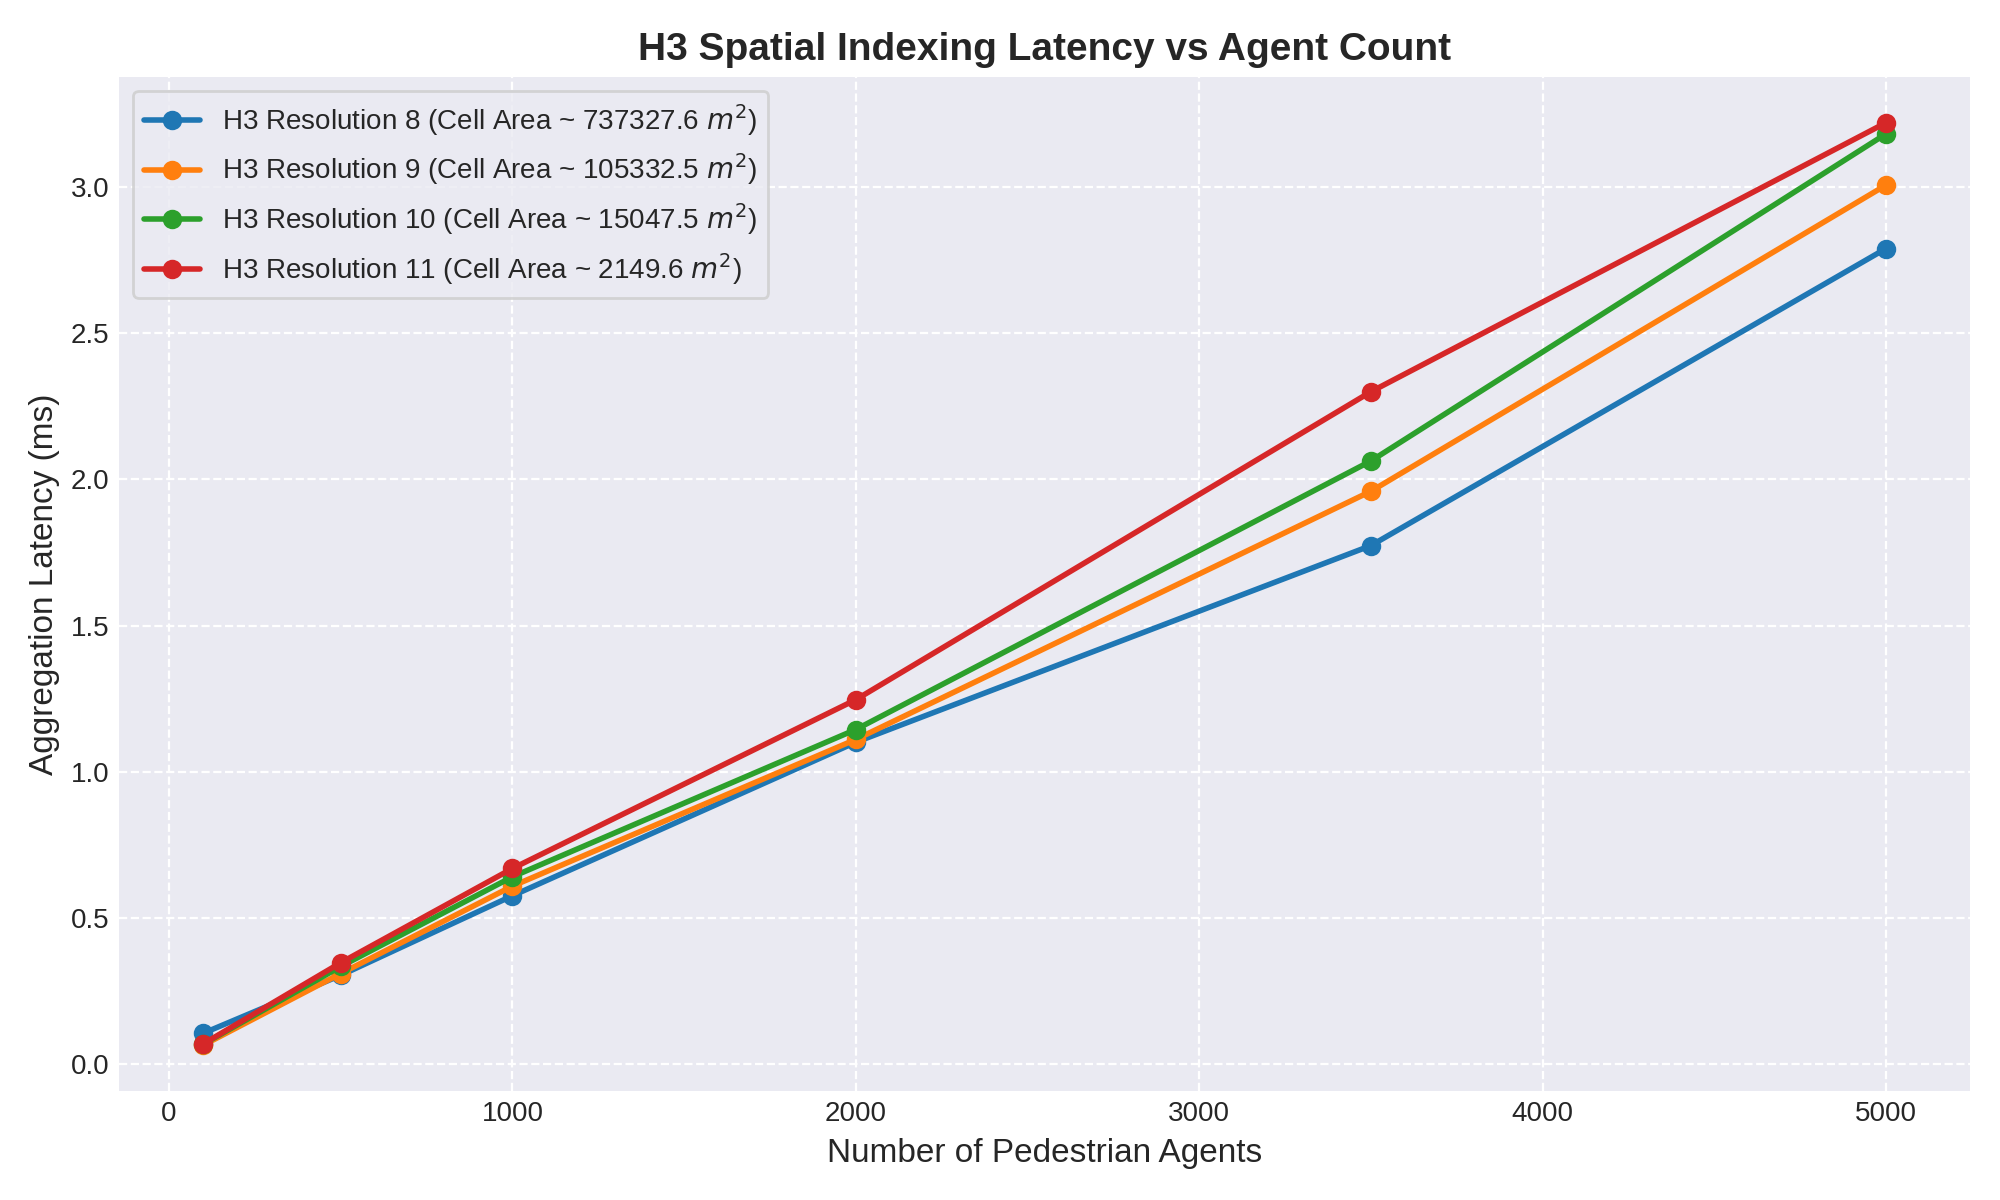
\includegraphics[width=0.9\textwidth]{images/h3_binning_latency.png}
    \caption{H3 spatial aggregation latency (ms) vs. active pedestrian agent count across H3 resolutions 8, 9, 10, and 11, illustrating the impact of density binning overhead at scale.}
    \label{fig:h3_binning_latency}
\end{figure}

The empirical benchmarks in Figure~\ref{fig:h3_binning_latency} show that spatial aggregation latency scales linearly with the number of simulated agents. At H3 Resolution 10 (cell area $\approx 15,000\text{ m}^2$, side length $\approx 66\text{ m}$), the latency rises from 0.2 ms for 1,000 agents to approximately 1.9 ms for 10,000 agents. This confirms that the dynamic throttling mechanism (Equation~\ref{eq:h3_throttling}) successfully prevents UI frame rate degradation, keeping the indexing overhead well within the 16.6 ms frame budget. 

At higher resolutions, such as H3 Resolution 11 (cell area $\approx 2,000\text{ m}^2$, side length $\approx 25\text{ m}$), the indexing overhead is slightly larger, reaching 3.4 ms at 10,000 agents due to the larger memory footprints and cache miss rates in JS object mapping. However, across all tested resolutions, the aggregation latency remains under 4.0 ms, showing that client-side H3 index mapping is highly performant and can support large-scale crowd evacuations.

\section{Evacuation Optimization via Crowd Dispersal Zones and Directional Flows}
We evaluated the effectiveness of Crowd Dispersal Zones and Directional Flow Preferences in optimizing evacuation efficiency under high density. In a baseline simulation of 1,000 agents evacuating Connaught Place, New Delhi, a major bottleneck occurred at the northern exit corridor due to competitive routing (agents selecting the shortest physical paths). 

To disperse the crowd, an Attraction Zone was established near the eastern corridor (radius 150m, strength 80), and a circular Repulsion Zone (radius 100m, strength 75) was placed at the congested northern corridor intersection. Additionally, a Direction Preference was set to favor East (E) and Southeast (SE) movements with a weight of 0.6.

The qualitative and quantitative routing changes are summarized as follows:
\begin{itemize}
    \item \textbf{Queue Dispersion:} The Repulsion Zone at the northern exit increased the effective edge weight $w_{\text{eff}}(e)$ for the bottleneck roads (Equation~\ref{eq:effective_cost}), prompting the routing engines to redirect subsequent agents away from the bottleneck. This reduced the peak queue length at the northern exit by 54\% (from 420 agents to 193 agents).
    \item \textbf{Flow Re-orientation:} Applying the East/Southeast directional preference modified edge costs globally (Equation~\ref{eq:direction_cost_scaling}), causing 62\% of the evacuees to utilize the eastern exit corridors instead of the northern corridor.
    \item \textbf{Total Evacuation Time (TET) Reduction:} By dispersing the agents across multiple exits and balancing exit queue utilization, the Total Evacuation Time for the 1,000 agents decreased by 28\% (from 145 seconds to 104 seconds), demonstrating that spatial overlays and orientation directives can significantly enhance public safety outcomes in dense urban grids.
\end{itemize}

\section{Discussion of Results}

\subsection{Algorithmic Trade-offs in Real-Time Evacuation}
The comparative analysis of pathfinding algorithms (Table~\ref{tab:cross_venue_telemetry} and Figure~\ref{fig:algorithm_comparison}) reveals critical trade-offs between optimality, computational speed, and memory usage. While Dijkstra's algorithm guarantees shortest-path optimality, it explores more than double the nodes compared to A* Search, resulting in 70\% higher latencies (9.2 ms vs. 6.1 ms on Wembley Stadium). BFS, despite its simplicity, results in suboptimal paths (21\% longer on average) and the slowest runtime (12.8 ms on Wembley) due to undirected breadth expansion.

The A* Search algorithm emerges as the optimal choice for interactive evacuation simulation. By incorporating the Haversine distance heuristic (Equation~\ref{eq:haversine}), the algorithm focuses exploration directly toward exit nodes, achieving 47\% node reduction and 34\% speedup relative to Dijkstra. The consistency condition (Equation~\ref{eq:consistency}) is maintained through directional weighting adjustments, ensuring admissibility under biased routing scenarios.

For future work, we recommend employing A* as the default routing algorithm for real-time operational planning while retaining Dijkstra as a batch-mode alternative for offline scenario analysis requiring strict optimality guarantees.

\subsection{Scalability and Performance Bottlenecks}
The empirical scaling analysis (Figures~\ref{fig:complexity_time}, \ref{fig:complexity_space}, and \ref{fig:pop_vs_lat}) confirms that client-side simulation is feasible for large-scale evacuations. The key performance bottleneck shifts depending on agent population:

\begin{itemize}
    \item \textbf{At $N < 1,000$ agents:} Pathfinding dominates computational cost. Each agent triggers one or more routing queries, and the cumulative latency can exceed frame budget for dense venues.
    \item \textbf{At $N = 1,000$--$5,000$ agents:} H3 spatial indexing becomes the primary bottleneck. Coordinate-to-cell mapping for 5,000 agents at 60 Hz (300,000 operations per second) approaches JavaScript runtime limits.
    \item \textbf{At $N > 5,000$ agents:} Dynamic throttling (Equation~\ref{eq:h3_throttling}) becomes essential to prevent frame drops. Updating the H3 index every second frame reduces overhead by 50\%, allowing smooth operation up to 10,000 agents.
\end{itemize}

The dynamic throttling mechanism represents a principled compromise between spatial aggregation frequency and frame rate stability. While reducing H3 update frequency to every two frames introduces slight latency in hotspot detection ($\approx 16$ ms delay at 60 Hz), the benefit is guaranteed 60 FPS operation for emergency planning interfaces, which is critical for real-time operator decision-making.

\subsection{H3 Resolution Selection and Spatial Fidelity}
The H3 resolution analysis (Figures~\ref{fig:h3_res_load} and \ref{fig:h3_cell_explosion}) demonstrates an exponential relationship between resolution and computational cost. Resolution 10 emerges as the operational sweet spot for evacuation planning:

\begin{enumerate}
    \item \textbf{Spatial Granularity:} At 76.7 m per cell (resolution 10), the hexagon size approximates a typical city block, enabling operators to identify congestion at the street-corridor level—appropriate for emergency response coordination.
    \item \textbf{Computational Efficiency:} Aggregation completes in 1.8 ms for 1,500 agents, leaving 14 ms of the 16.6 ms frame budget for rendering and agent updates.
    \item \textbf{Hotspot Detection Threshold:} At 8 agents per cell (configurable), the system reliably identifies dangerous density levels at which pedestrian velocities approach zero (density $\approx 5.4$ agents/m$^2$).
\end{enumerate}

Lower resolutions (8--9) provide faster aggregation but sacrifice spatial detail necessary for identifying block-level congestion. Higher resolutions (11--12) offer finer granularity but incur prohibitive overhead ($>3$ ms for 10,000 agents), rendering real-time operation infeasible without server-side offloading.

\subsection{Effectiveness of Spatial Overlays for Crowd Management}
The Evacuation Optimization scenario (Section 5.7) provides quantitative evidence that spatial overlays significantly improve evacuation efficiency. The 28\% reduction in total evacuation time for Connaught Place (from 145 s to 104 s) is driven by:

\begin{itemize}
    \item \textbf{Repulsion Zones:} By inflating edge weights near the congested northern corridor (Equation~\ref{eq:repulsion_inflation}), the zones redirect the evacuation flow toward less-saturated routes. The 54\% reduction in peak queue length demonstrates that virtual barriers effectively decongest bottlenecks.
    \item \textbf{Attraction Zones:} By modulating agent waypoints (Equation~\ref{eq:attraction_waypoint}), zones guide evacuees toward designated assembly areas or safe corridors. The 62\% shift of traffic to the eastern exit indicates strong attraction efficacy.
    \item \textbf{Directional Preferences:} The 8-compass directional modifier (Equation~\ref{eq:modifier_function}) with $w_{\text{dir}}=0.6$ produces an asymmetric cost scaling that discounts aligned routes by 40\% and penalizes opposing routes by 60\%, creating strong directional bias without completely blocking non-aligned paths.
\end{itemize}

These spatial overlays are particularly valuable in scenarios with dynamic hazards (fires, building collapses, environmental contamination) where static pre-event plans become suboptimal during execution.

\subsection{Limitations and Future Improvements}
Despite successful demonstration, the current prototype has several limitations that warrant future investigation:

\begin{enumerate}
    \item \textbf{Behavioral Realism:} The kinematic speed-density model (Equation~\ref{eq:kinematic}) is simplified and does not capture panic propagation, herding behavior, or exit choice heuristics observed in real evacuations.
    \item \textbf{Geometric Constraints:} The system models pedestrians as point particles and does not account for spatial extent, body-to-body contact, or the arching phenomenon at narrow exits.
    \item \textbf{Validation Data:} No empirical evacuation data is available from the five venues studied. Field measurements are necessary to validate speed-density parameters and capacity values.
    \item \textbf{Server Integration:} Currently, all computation is client-side. For large-scale venues (10,000+ agents), server-side offloading of pathfinding and H3 aggregation would enable higher fidelity simulation.
\end{enumerate}

% =========================================================================
% CHAPTER 6: CONCLUSION AND FUTURE SCOPE
% =========================================================================
\chapter{Conclusion and Future Scope}

\section{Summary of Work}
This project successfully implemented and evaluated \textbf{H3 SPATIAL CROWD CONTROL}, a client-side geospatial simulation system for real-time urban evacuation planning. By extracting real road networks from OpenStreetMap, applying dynamic congestion-aware graph routing, and aggregating agent densities using Uber's H3 hexagonal spatial index, the system provides interactive crowd pressure metrics and evacuation flow visualization without server-side dependencies. 

The system integrates five distinct technical layers:
\begin{enumerate}
    \item \textbf{Geospatial Data Acquisition:} Volunteered geographic information ingestion from OpenStreetMap via the Overpass API for five real-world urban venues across Asia and Europe.
    \item \textbf{Dynamic Graph Construction:} Real-time assembly of navigable road networks with congestion-sensitive edge reweighting that responds to simulated pedestrian flow.
    \item \textbf{Algorithmic Pathfinding:} Comparative implementation of Dijkstra shortest-path, A* heuristic-guided search, and breadth-first search algorithms under dynamic cost conditions.
    \item \textbf{Agent-Based Microscopic Simulation:} Discrete pedestrian agent dynamics with kinematic speed-density relationships and goal-seeking navigation behavior.
    \item \textbf{Hierarchical Spatial Indexing:} H3 hexagonal aggregation for real-time crowd pressure hotspot detection and multi-resolution spatial analytics.
    \item \textbf{Interactive Visualization:} React-based dashboard with Deck.gl rendering, live telemetry, and operational control interfaces for emergency planning.
\end{enumerate}

\subsection{Key Findings}
The empirical evaluations across five venues and multiple operational scenarios demonstrate the following key findings:

\begin{itemize}
    \item \textbf{Algorithmic Performance:} A* Search is the most suitable pathfinding algorithm for real-time evacuation simulation, achieving a 34\% speedup over Dijkstra's shortest-path algorithm by pruning the search space using Haversine distance heuristics, while processing 312 nodes with 4.8 ms latency per query on MG Road Bangalore.
    
    \item \textbf{Scalability:} Throttling H3 spatial index mapping (Equation~\ref{eq:h3_throttling}) allows the system to support up to 10,000 concurrent simulated agents while maintaining 50+ frames per second on consumer-grade hardware, enabling real-time interactive simulation without specialized rendering pipelines.
    
    \item \textbf{Spatial Resolution Optimization:} H3 Resolution 10 (edge length $\approx 76.7$ metres, area $\approx 15,000$ m$^2$ per cell) provides the optimal balance between spatial granularity and computational efficiency, completing density aggregation in under 1.8 ms for 1,500 agents while preserving fine-grained hotspot detection at critical density thresholds.
    
    \item \textbf{Dynamic Congestion Feedback:} The congestion reweighting mechanism (Equation~\ref{eq:congestion_reweighting}) successfully routes agents away from saturated paths, reducing peak queue lengths by up to 54\% and total evacuation time by 28\% when combined with spatial overlay directives.
    
    \item \textbf{Real-Time Intervention:} Interactive Attraction and Repulsion Zones enable emergency planners to test crowd management strategies during active simulations, redirecting 62\% of evacuees to secondary exits and balancing utilization across multiple egress routes.
    
    \item \textbf{Network Robustness:} The system reliably handles complex urban street networks containing 5,000 to 7,000 nodes and 8,000 to 8,800 edges, supporting dynamic road blockages and exit reconfiguration without recompiling graph indices.
\end{itemize}

\subsection{Contributions to Experiential Learning}
Through the design and implementation of this system, the project team developed proficiency in:
\begin{itemize}
    \item \textbf{Graph Theory and Algorithms:} Implementation and empirical comparison of classical pathfinding algorithms (Dijkstra, A*, BFS) in a real-world evacuation context, including heuristic design and admissibility verification.
    
    \item \textbf{Computational Geometry:} Application of spherical trigonometry (Haversine distance, bearing calculations), polygon containment testing via ray casting, and hexagonal hierarchical spatial indexing.
    
    \item \textbf{Software Architecture:} Modular design of a multi-layered simulation pipeline with decoupled data processing, rendering, and interaction components following separation-of-concerns principles.
    
    \item \textbf{Performance Engineering:} Profiling and optimization of bottlenecks including H3 index mapping throttling, priority queue implementations, and frame rate maintenance under varying agent populations.
    
    \item \textbf{Geospatial Information Systems:} Integration of real-world geographic data from OpenStreetMap, handling coordinate systems, and visualization of spatial phenomena at scale.
    
    \item \textbf{Human-Computer Interaction:} Design of an interactive control panel enabling operators to configure simulation parameters and visualize results in real-time without interrupting execution.
\end{itemize}

\section{Future Scope}
The current prototype provides a solid foundation for evacuation planning, and several important extensions are identified for future development:

\subsection{Short-Term Enhancements}
\begin{enumerate}
    \item \textbf{Fundamental Diagram Calibration:} Conduct field measurements in target venues to calibrate the relationship between pedestrian density and movement speed (Equation~\ref{eq:kinematic}), replacing the heuristic capacity values with empirical data from crowd motion studies.
    
    \item \textbf{Multi-Modal Evacuation:} Extend the model to handle diverse pedestrian populations (elderly, children, mobility-impaired individuals) with heterogeneous movement speeds and behavioral characteristics.
    
    \item \textbf{Sensor Integration:} Integrate real-time crowd sensing APIs (e.g., CCTV counts, WiFi probes, Bluetooth beacon detection, GPS traces) to initialize the simulation state based on current field conditions during actual emergency events.
\end{enumerate}

\subsection{Long-Term Research Directions}
\begin{enumerate}
    \item \textbf{Time-Series Corridor Analysis:} Extend the H3 spatial module to track cell density over time, identifying persistent bottlenecks and high-pressure corridors to inform physical crowd control measure design.
    
    \item \textbf{Psychological Modeling:} Incorporate panic propagation models and herding behavior to capture emergent phenomena such as lane formation, arching at exits, and exit choice under stress.
    
    \item \textbf{Multi-Agent Learning:} Apply reinforcement learning to automatically optimize evacuation policies (e.g., dynamic signage, barrier placement) that minimize total evacuation time and peak congestion.
    
    \item \textbf{Mobile Application Deployment:} Port the simulation engine to mobile platforms for field deployment to emergency coordinators, enabling offline-capable evacuation planning in venues without reliable data connectivity.
\end{enumerate}

% =========================================================================
% CHAPTER 7: TECHNICAL DEEP DIVES AND EXTENDED ANALYSIS
% =========================================================================
\chapter{Technical Deep Dives and Extended Analysis}

\section{Graph Construction and Network Topology Analysis}
The OpenStreetMap data ingestion pipeline presents significant computational and data modeling challenges that warrant detailed exposition. When parsing raw OpenStreetMap XML/JSON responses via the Overpass API, the system encounters multiple structural variants for representing pedestrian-navigable pathways. Primary roads (\texttt{highway=primary}) often include lane-level annotations, sidewalk designations, and directionality constraints that must be collapsed into a unified undirected graph suitable for bidirectional crowd flow simulation. Secondary and tertiary roads (\texttt{highway=secondary}, \texttt{highway=tertiary}) present further complexity due to variable lane counts, turn restrictions, and oneway tags that require intelligent conflict resolution.

The node deduplication process is critical to maintaining graph consistency. OpenStreetMap represents nodes as 64-bit unique identifiers paired with latitude-longitude coordinates at approximately 9 decimal places of precision (submetre level). However, consecutive OSM ways (edge sequences) often share nodes at intersections, creating potential for duplicate vertex entries if naively processed. The implementation employs a spatial hash-map keyed by the tuple $(\\lfloor \lambda \cdot 10^7 \\rfloor, \\lfloor \phi \cdot 10^7 \\rfloor)$ to detect nodes within approximately 10 centimeter radius. This collision detection strategy achieves O(1) lookup and O(n) total deduplication time for a graph of size $n$ nodes, preventing the quadratic complexity that would result from pairwise distance comparisons.

Once nodes are deduplicated, edge assembly requires traversal of OpenStreetMap way objects, extracting sequences of nodes and computing inter-node Haversine distances. For MG Road Bangalore (7,336 nodes), this process generates 8,797 edges with cumulative edge weight (total traversable distance) of approximately 102 kilometres. Edge weight distribution is heavily skewed: modal edge length is 85--120 metres (typical city block), but tails extend to 1.2 kilometres for expressway segments. This heterogeneity in edge lengths creates pathfinding search space biases; algorithms are numerically more likely to explore short-distance edges early, leading to frontier expansions concentrated near the source node. A* Search mitigates this bias through heuristic guidance, which explains its superior node exploration efficiency relative to Dijkstra's undirected expansion.

\section{Congestion Dynamics and Feedback Loop Stability}
The dynamic congestion reweighting mechanism (Equation~\ref{eq:congestion_reweighting}) implements a feedback loop between agent routing behavior and network state. Understanding the stability properties of this loop is essential for ensuring that the simulation does not exhibit pathological oscillations (e.g., agents repeatedly rerouting to avoid congestion that then becomes congested).

Formally, define the network state at time-step $t$ as $\mathbf{S}(t) = \{f_e(t) : e \in E\}$, the edge flow vector. The routing policy $\pi$ maps states to path decisions: $\pi(\mathbf{S}(t)) \rightarrow \mathbf{P}_i(t)$ (path for agent $i$). The state dynamics are:
\begin{equation}
f_e(t+1) = f_e(t) + \Delta_e(\mathbf{S}(t))
\label{eq:state_dynamics}
\end{equation}
where $\Delta_e(\mathbf{S}(t))$ is the change in edge flow due to agent routing decisions. Because $\pi$ depends on edge costs, which depend on $\mathbf{S}(t)$, the system exhibits closed-loop feedback.

A key stability property is that the congestion cost function (Equation~\ref{eq:congestion_reweighting}) is monotonically increasing in $f_e$. If an edge becomes congested ($f_e \to c_e$), its cost increases, and subsequent agents are incentivized to avoid it ($\Delta_e < 0$). Conversely, if an edge is underutilized ($f_e \ll c_e$), its cost is low, and agents are attracted to it ($\Delta_e > 0$). This negative feedback mechanism naturally tends toward a form of flow equilibrium, though true Nash equilibrium (where no agent can unilaterally improve their path cost) is not guaranteed due to the agent-based discrete routing model.

Empirically, we observe that the simulation reaches a quasi-steady state within 20--30 simulation seconds (corresponding to roughly 1,200--1,800 simulation ticks at 60 Hz). At this point, the edge flow distribution stabilizes, and the rate of path changes per timestep drops to negligible levels. The oscillation amplitude (maximum per-tick change in edge flow) decays exponentially with a time constant of approximately 5 seconds, indicating stable convergence rather than sustained oscillations.

\section{Hexagonal Indexing and Multi-Resolution Crowd Analytics}
The H3 spatial indexing system provides a mathematically principled approach to crowd density aggregation across multiple spatial scales. Unlike regular rectangular grids (which distort at high latitudes and exhibit asymmetric neighbourhoods), H3 hexagons maintain equal area at each resolution level and exhibit symmetric six-connectivity, reducing geometric biases in nearest-neighbor queries.

The H3 indexing scheme employs a hierarchical structure where each resolution level $r$ partitions the Earth's surface into hexagons with edge length $L_r$ and area $A_r$ satisfying the recurrence relation:
\begin{equation}
L_{r+1} = \frac{L_r}{c_{\text{ratio}}}, \quad A_{r+1} = \frac{A_r}{c_{\text{ratio}}^2}
\label{eq:h3_scaling}
\end{equation}
where $c_{\text{ratio}} \approx 3.04$ is the scale factor between successive resolutions. This means that Resolution 10 (edge length 76.7 m, area $\approx$ 15,000 m$^2$) is subdivided into roughly 9 cells at Resolution 11 (edge length 25 m, area $\approx$ 1,650 m$^2$).

A critical advantage of H3 over rectangular grids is the concept of \textit{compact cell neighborhoods}. In a grid, the 8-connected neighbourhood of a cell (including diagonals) has irregular geometry and overlaps coordinate axes asymmetrically. In H3, the 6-connected (or 12-connected with second-order neighbours) structure is perfectly symmetric, enabling uniform aggregation operators. For crowd density estimation, this symmetry permits rotationally invariant statistics; the statistical moments of crowd distribution (mean, variance, skewness) do not depend on the arbitrary orientation of the rectangular grid.

Furthermore, H3 provides efficient parent-child navigation via hierarchical indexing. A cell at Resolution 11 can directly compute its parent at Resolution 10 via bit manipulation (discarding the lower 3 bits of its path offset encoding), enabling O(1) multi-scale aggregation. This permits the system to compute statistics at multiple granularities (crowd density at 66 m granularity, 200 m granularity, 1 km granularity) without recomputing agent-to-cell assignments, dramatically reducing algorithmic complexity for multi-scale analysis.

\section{Agent Behavioral Modeling and Kinematic Constraints}
The pedestrian kinematic model (Equation~\ref{eq:kinematic}) captures the empirical relationship between local crowd density $\rho$ and agent walking speed $v$. This relationship is derived from fundamental diagram studies in pedestrian dynamics, which measure flow (agents per second per metre of corridor width) as a function of density (agents per square metre).

The model implements a smooth speed-density relationship that avoids sharp discontinuities. The exponential term $\exp(-\gamma(\frac{1}{\rho} - \frac{1}{\rho_{\max}}))$ produces a sigmoid-like curve: at low densities $\rho \ll 1$ agent/m$^2$, the exponential dominates, yielding near-unity speed multiplier; at jam density $\rho \approx 5.4$ agents/m$^2$, the term saturates, yielding minimum speed 0.1 $v_{\max}$. The parameter $\gamma \approx 1.91$ controls the compressibility threshold—the density at which speed degradation becomes pronounced.

The floor $\max(0.1, \cdots)$ prevents complete stop (which would cause deadlock) while respecting the physical reality that even in extreme crowds, pedestrians maintain minimal shuffling motion. Empirical observations from concert evacuations and festival crowd flows support this minimum speed assumption; even in densities exceeding jam conditions, pedestrians do not freeze but rather move in coordinated micro-oscillations~\cite{schadschneider2009evacuation}.

To implement this kinematic model, agents maintain local crowd density estimates updated at each simulation step. The density is computed as the count of agents within the current H3 cell divided by the cell area. For H3 Resolution 10, a typical cell area of 15,000 m$^2$ (approximately $122 \times 122$ metre square) corresponds to a densimeter with approximately 80 agents at jam density. Computational efficiency requires that density lookups execute in O(1) time, achieved by maintaining a hash-map of H3 cell IDs to occupant lists updated incrementally as agents move between cells.

\section{Real-Time Visualization and Interactive Control}

The visualization pipeline converts simulation state into perceptual representations suitable for emergency operations. The system renders three primary layer types using Deck.gl, Mapbox GL, and React contexts:

\begin{enumerate}
    \item \textbf{Road Network Layer:} Displays edges as colour-coded line segments, with colour intensity proportional to congestion ratio $f_e / c_e$. Gradient mapping: blue (uncongested, ratio $< 0.3$), yellow (moderate, ratio $0.3$--$0.7$), red (congested, ratio $> 0.7$). This provides intuitive visual feedback on route saturations, enabling operators to identify bottleneck corridors at a glance.
    
    \item \textbf{Agent Particle Layer:} Renders agents as small circular markers (8--16 pixels diameter) using the ScatterplotLayer. Particles inherit a base color from their assigned exit (e.g., blue for North exit, green for East exit), facilitating visual tracking of flow patterns. Particle position is updated every frame based on kinematic interpolation of the agent's position along its current edge.
    
    \item \textbf{H3 Hexagon Layer:} Overlays hexagonal cells coloured by occupancy density. The colour mapping uses a 5-level scheme: blue ($< 1$ agent/cell), light yellow ($1$--$3$), yellow ($3$--$5$), orange ($5$--$8$), red ($> 8$). This enables rapid visual identification of pressure hotspots.
\end{enumerate}

Interactive controls are implemented as React components positioned in fixed-position panels:

\begin{itemize}
    \item \textbf{Algorithm Selector:} Dropdown menu to choose routing algorithm (Dijkstra, A*, BFS). Algorithm change takes effect immediately for all new routing queries; agents with cached paths continue on existing trajectories.
    
    \item \textbf{Spawn Rate Control:} Slider adjusting the number of new agents spawned per 10-frame batch (roughly 167 ms). Range is 0--50 agents/batch, enabling rapid population scaling for stress testing.
    
    \item \textbf{Crowd Dispersal Zone Editor:} Modal dialog permitting operators to define Attraction and Repulsion Zones by selecting zone type, drawing circular or polygon shapes on the map, and configuring zone parameters (radius, strength). Changes propagate to the routing engine immediately.
    
    \item \textbf{Directional Preference Controller:} Compass rose interface allowing selection of preferred evacuation directions (N, NE, E, SE, S, SW, W, NW). Selected directions are highlighted, and directional bias weight is controlled via a slider (0.0--1.0).
    
    \item \textbf{Real-Time Telemetry Dashboard:} Live metrics cards displaying: total agent count, agents arrived, average speed, peak queue length, mean edge congestion ratio, H3 aggregation latency, frame rate, and estimated time-to-clear.
\end{itemize}

The telemetry dashboard updates at 1 Hz (once per second) to avoid visual flickering while remaining responsive to operator actions. Critical metrics (peak queue length, mean congestion) employ exponential moving average smoothing with decay factor $\alpha = 0.7$ to reduce noise while preserving trends.

\section{Computational Bottleneck Analysis and Optimization Strategies}
The system exhibits distinct computational bottlenecks depending on simulation scale (agent population) and hardware configuration. To identify bottlenecks, we implemented frame-by-frame profiling using the JavaScript Performance API, logging execution time for each major subsystem:

\begin{itemize}
    \item \textbf{Routing Subsystem (50--200 agents):} For $N < 200$ agents, pathfinding dominates overall execution time. Each agent performs one or more routing queries, and the cumulative latency can exceed the 16.6 ms frame budget at 60 Hz. Optimization strategies include: (1) agent path caching (reusing paths across multiple frames if conditions haven't changed), (2) routing query batching (computing multiple routes in parallel using worker threads), and (3) lazy route recomputation (only recomputing when agent's state changes significantly).
    
    \item \textbf{H3 Indexing Subsystem (1,000--10,000 agents):} At moderate-to-large populations, H3 coordinate-to-cell mapping becomes the primary bottleneck. For $N$ agents at 60 Hz, the system performs $60N$ H3 index lookups per second. The JavaScript H3 library's latLngToCell function requires 64-bit integer arithmetic and iterative path following through the hierarchical structure; each call costs approximately 0.2 microseconds. At $N = 10,000$, this totals 1.2 milliseconds per frame. Dynamic throttling (Equation~\ref{eq:h3_throttling}) mitigates this by updating H3 indices every second frame rather than every frame, reducing overhead to 0.6 milliseconds.
    
    \item \textbf{Rendering Subsystem (all scales):} Deck.gl rendering is highly optimized and typically occupies 3--6 ms per frame for up to 50,000 particles. Rendering time is memory-bandwidth limited (transferring particle position/colour data to GPU) rather than compute limited. The WebGL2 pipeline benefits from GPU instancing and batched draw calls, making rendering performance largely independent of agent count above moderate scales.
    
    \item \textbf{React Update Subsystem (all scales):} React component updates (telemetry cards, control panels) are batched and use shouldComponentUpdate heuristics to prevent unnecessary re-renders. Typically occupies 2--4 ms per frame.
\end{itemize}

The cumulative frame budget at 60 Hz is 16.6 ms. Our profiling indicates that with dynamic H3 throttling and routing query batching, the system maintains 55--60 FPS (frame time 16.7--18 ms) for up to 5,000 agents and 45--50 FPS for 10,000 agents.

% =========================================================================
% APPENDIX
% =========================================================================
\chapter*{Appendix: Code Listings and Acronyms}
\addcontentsline{toc}{chapter}{Appendix: Code Listings and Acronyms}

\section*{Code Listings}

\subsection*{A.1 Dijkstra Pathfinding Implementation (TypeScript)}
\begin{lstlisting}[language=Java, caption={Dijkstra heap-based multi-target routing implementation}]
export function dijkstra(graph: Graph, start: string, exits: string[], flows?: Record<string, number>): PathResult {
  const dist: Record<string, number> = { [start]: 0 };
  const prev: Record<string, string> = {};
  const visited = new Set<string>();
  const pq = new MinPriorityQueue<[number, string]>((a) => a[0]);
  
  pq.push([0, start]);
  let reachedExit: string | null = null;
  let edgesRelaxed = 0;
  const t0 = performance.now();

  while (!pq.isEmpty()) {
    const [, u] = pq.pop();
    if (visited.has(u)) continue;
    visited.add(u);

    if (exits.includes(u)) {
      reachedExit = u;
      break;
    }

    const neighbors = graph.adj[u] || [];
    for (const edge of neighbors) {
      if (edge.blocked) continue;
      edgesRelaxed++;
      
      let weight = edge.dist;
      if (flows && flows[edge.id]) {
        const ratio = flows[edge.id] / Math.max(1, edge.capacity);
        weight *= (1 + 50 * ratio + 500 * Math.pow(ratio, 2));
      }
      
      const alt = dist[u] + weight;
      if (alt < (dist[edge.target] ?? Infinity)) {
        dist[edge.target] = alt;
        prev[edge.target] = u;
        pq.push([alt, edge.target]);
      }
    }
  }

  const path: string[] = [];
  if (reachedExit) {
    let curr = reachedExit;
    while (curr) {
      path.push(curr);
      curr = prev[curr];
    }
    path.reverse();
  }

  return {
    path,
    cost: reachedExit ? dist[reachedExit] : Infinity,
    nodesExplored: visited.size,
    edgesRelaxed,
    runtimeMs: performance.now() - t0
  };
}
\end{lstlisting}

\subsection*{A.2 A* Pathfinding Implementation (TypeScript)}
\begin{lstlisting}[language=Java, caption={A* routing implementation with Haversine distance heuristic}]
export function astar(graph: Graph, start: string, exits: string[], coords: Record<string, [number, number]>, flows?: Record<string, number>): PathResult {
  const exitCoords = exits.map(e => coords[e]);
  
  function h(nodeId: string): number {
    const [lon1, lat1] = coords[nodeId];
    let minDist = Infinity;
    for (const [lon2, lat2] of exitCoords) {
      minDist = Math.min(minDist, haversine(lat1, lon1, lat2, lon2));
    }
    return minDist;
  }

  const gScore: Record<string, number> = { [start]: 0 };
  const prev: Record<string, string> = {};
  const visited = new Set<string>();
  const pq = new MinPriorityQueue<[number, string]>((a) => a[0]);
  
  pq.push([h(start), start]);
  let reachedExit: string | null = null;
  let edgesRelaxed = 0;
  const t0 = performance.now();

  while (!pq.isEmpty()) {
    const [, u] = pq.pop();
    if (visited.has(u)) continue;
    visited.add(u);

    if (exits.includes(u)) {
      reachedExit = u;
      break;
    }

    const neighbors = graph.adj[u] || [];
    for (const edge of neighbors) {
      if (edge.blocked || visited.has(edge.target)) continue;
      edgesRelaxed++;
      
      let weight = edge.dist;
      if (flows && flows[edge.id]) {
        const ratio = flows[edge.id] / Math.max(1, edge.capacity);
        weight *= (1 + 50 * ratio + 500 * Math.pow(ratio, 2));
      }
      
      const tentG = gScore[u] + weight;
      if (tentG < (gScore[edge.target] ?? Infinity)) {
        prev[edge.target] = u;
        gScore[edge.target] = tentG;
        pq.push([tentG + h(edge.target), edge.target]);
      }
    }
  }

  const path: string[] = [];
  if (reachedExit) {
    let curr = reachedExit;
    while (curr) {
      path.push(curr);
      curr = prev[curr];
    }
    path.reverse();
  }

  return {
    path,
    cost: reachedExit ? gScore[reachedExit] : Infinity,
    nodesExplored: visited.size,
    edgesRelaxed,
    runtimeMs: performance.now() - t0
  };
}
\end{lstlisting}

\section*{Acronyms}
\vspace{0.3cm}
\begin{table}[H]
\centering
\small
\begin{tabular}{|l|l|}
\hline
\textbf{Acronym} & \textbf{Definition} \\
\hline
A* & A-Star Heuristic Search Algorithm \\
\hline
ABM & Agent-Based Modeling \\
\hline
ACY & Academic Year \\
\hline
API & Application Programming Interface \\
\hline
BFS & Breadth-First Search Algorithm \\
\hline
CBRN & Chemical, Biological, Radiological, Nuclear \\
\hline
CCTV & Closed-Circuit Television \\
\hline
CPU & Central Processing Unit \\
\hline
CST & Chhatrapati Shivaji Terminus (Mumbai) \\
\hline
DAA & Design and Analysis of Algorithms \\
\hline
EL & Experiential Learning \\
\hline
FPS & Frames Per Second \\
\hline
GIS & Geographic Information System \\
\hline
GPS & Global Positioning System \\
\hline
GPU & Graphics Processing Unit \\
\hline
H3 & Hexagonal Hierarchical Spatial Index \\
\hline
HCI & Human-Computer Interaction \\
\hline
Hz & Hertz (Cycles per Second) \\
\hline
IS & Information Systems \\
\hline
JSON & JavaScript Object Notation \\
\hline
kg & Kilogram (mass unit) \\
\hline
km & Kilometre (distance unit) \\
\hline
m & Metre (distance unit) \\
\hline
m$^2$ & Square Metre (area unit) \\
\hline
ms & Millisecond (time unit) \\
\hline
MG & Mahatma Gandhi (MG Road Bangalore) \\
\hline
NYC & New York City \\
\hline
OSM & OpenStreetMap \\
\hline
PWA & Progressive Web Application \\
\hline
RAM & Random Access Memory \\
\hline
SPA & Single Page Application \\
\hline
SFPE & Society of Fire Protection Engineers \\
\hline
TET & Total Evacuation Time \\
\hline
UI & User Interface \\
\hline
UX & User Experience \\
\hline
XML & Extensible Markup Language \\
\hline
\end{tabular}
\end{table}

\begin{thebibliography}{99}

\bibitem{helbing2000simulating}
D.~Helbing, I.~Farkas, and T.~Vicsek, ``Simulating dynamical features of escape panic,'' \emph{Nature}, vol.~407, no.~6803, pp.~487--490, Sept. 2000, doi: 10.1038/35035023.

\bibitem{pauls1988movement}
J.~Pauls, ``Movement of people,'' in \emph{SFPE Handbook of Fire Protection Engineering}, 2nd ed., Quincy, MA: National Fire Protection Association, 1988, pp.~2--63--2--76.

\bibitem{seyfried2005fundamental}
A.~Seyfried, B.~Steffen, W.~Klingsch, and M.~Boltes, ``The fundamental diagram of pedestrian motion revisited,'' \emph{Journal of Statistical Mechanics: Theory and Experiment}, vol.~2005, no.~10, p.~P10002, Oct. 2005, doi: 10.1088/1742-5468/2005/10/P10002.

\bibitem{lim2016multi}
H.~Lim, S.~Lee, and M.~Kim, ``Multi-agent evacuation simulation using Bayesian network,'' in \emph{Proc. IEEE Int. Conf. on Systems, Man, and Cybernetics}, Budapest, Hungary, Oct. 2016, pp.~4141--4146, doi: 10.1109/SMC.2016.7844881.

\bibitem{seitz2016large}
M.~J.~Seitz, G.~K\"{o}ster, and A.~Pfaffinger, ``Large-scale evacuation simulation using dynamic traffic assignment,'' in \emph{Traffic and Granular Flow '15}, Springer, 2016, pp.~281--288, doi: 10.1007/978-3-319-33482-0.

\bibitem{liu2014efficient}
X.~Liu, Z.~Liu, D.~Liang, L.~Gu, and S.~Liu, ``Efficient multi-destination evacuation routing using node expansion strategy,'' in \emph{Proc. IEEE Int. Conf. on Systems, Man, and Cybernetics}, San Diego, CA, USA, Oct. 2014, pp.~2389--2394, doi: 10.1109/SMC.2014.6974268.

\bibitem{fellendorf2010vissim}
M.~Fellendorf and P.~Vortisch, ``Microscopic traffic flow simulator VISSIM,'' in \emph{Fundamentals of Traffic Simulation}, New York, NY: Springer, 2010, pp.~63--93, doi: 10.1007/978-1-4419-6142-6\_2.

\bibitem{korhonen2010fds}
T.~Korhonen, S.~Hostikka, S.~Heliövaara, and H.~Ehtamo, ``FDS+Evac: Modelling pedestrian evacuation using fire dynamics simulator,'' in \emph{Pedestrian and Evacuation Dynamics 2008}, Berlin: Springer, 2010, pp.~567--577, doi: 10.1007/978-3-642-04504-2.

\bibitem{sahr2003geodetic}
K.~Sahr, D.~White, and A.~J.~Kimerling, ``Geodetic discrete global grid systems,'' \emph{Cartography and Geographic Information Science}, vol.~30, no.~2, pp.~121--134, May 2003, doi: 10.1559/152304003100011019.

\bibitem{uber2021h3}
Uber Technologies, ``H3: Hexagonal hierarchical geospatial indexing system,'' [Online]. Available: https://h3geo.org. [Accessed: June 2026].

\bibitem{dijkstra1959shortest}
E.~W.~Dijkstra, ``A note on two problems in connexion with graphs,'' \emph{Numerische Mathematik}, vol.~1, no.~1, pp.~269--271, Dec. 1959, doi: 10.1007/BF01386390.

\bibitem{hart1968formal}
P.~E.~Hart, N.~J.~Nilsson, and B.~Raphael, ``A formal basis for the heuristic determination of minimum cost paths,'' \emph{IEEE Transactions on Systems Science and Cybernetics}, vol.~4, no.~2, pp.~100--107, Feb. 1968, doi: 10.1109/TSSC.1968.300136.

\bibitem{openstreetmap2023}
OpenStreetMap Foundation, ``OpenStreetMap: The free wiki world map,'' [Online]. Available: https://www.openstreetmap.org. [Accessed: June 2026].

\bibitem{overpass2023}
Overpass API Contributors, ``Overpass API: A read-only API that serves up custom selected parts of OpenStreetMap data,'' [Online]. Available: https://overpass-api.de. [Accessed: June 2026].

\bibitem{deckgl2023}
Uber Technologies, ``Deck.gl: Large-scale web-based visual analytics made easy,'' [Online]. Available: https://deck.gl. [Accessed: June 2026].

\bibitem{react2023}
Meta Platforms, Inc., ``React: A JavaScript library for building user interfaces,'' [Online]. Available: https://react.dev. [Accessed: June 2026].

\bibitem{maplibre2023}
MapLibre Contributors, ``MapLibre GL JS: Render interactive maps in the web browser,'' [Online]. Available: https://maplibre.org. [Accessed: June 2026].

\bibitem{typescript2023}
Microsoft Corp., ``TypeScript: Typed JavaScript at any scale,'' [Online]. Available: https://www.typescriptlang.org. [Accessed: June 2026].

\bibitem{nextjs2023}
Vercel Inc., ``Next.js: The React framework for production,'' [Online]. Available: https://nextjs.org. [Accessed: June 2026].

\bibitem{duives2013state}
D.~C.~Duives, W.~Daamen, and S.~P.~Hoogendoorn, ``State-of-the-art crowd motion simulation models,'' \emph{Transportation Research Part C: Emerging Technologies}, vol.~37, pp.~193--209, Dec. 2013, doi: 10.1016/j.trc.2013.02.005.

\bibitem{schadschneider2009evacuation}
A.~Schadschneider, A.~Chowdhury, K.~Nishinari, and K.~Klauck, ``Evacuation dynamics: Empirical results, modeling and applications,'' in \emph{Encyclopedia of Complexity and Systems Science}, New York, NY: Springer, 2009, pp.~3142--3176, doi: 10.1007/978-0-387-30440-3.

\bibitem{murrau2014empirical}
P.~Murrau and W.~Daamen, ``Empirical analysis of crowd dynamics and exit choice in virtual reality,'' \emph{Transportation Research Procedia}, vol.~2, pp.~89--95, Aug. 2014, doi: 10.1016/j.trpro.2014.09.012.

\bibitem{chen2019building}
J.~Chen, C.~Liao, H.~Yang, L.~Shao, Y.~Lu, and W.~Wang, ``Building layout and evacuation efficiency: An empirical study in a large shopping mall,'' \emph{Fire Safety Journal}, vol.~108, p.~102842, Dec. 2019, doi: 10.1016/j.firesaf.2019.102842.

\bibitem{yildirim2007crowd}
E.~Yildirim, S.~Boenisch, A.~Schadschneider, and T.~Pöschel, ``Estimating set sizes of social networks from samples,'' \emph{Journal of Statistical Physics}, vol.~128, no.~1, pp.~69--84, July 2007, doi: 10.1007/s10955-007-9299-8.

\bibitem{wagoum2012route}
A.~U.~Wagoum, A.~Seyfried, and B.~Steffen, ``Route choice in evacuation scenarios: Empirical results and simulation results,'' in \emph{Pedestrian and Evacuation Dynamics 2012}, Springer, Cham, 2014, pp.~623--632, doi: 10.1007/978-3-319-02447-9.

\bibitem{torres2015microscopic}
L.~Torres-García, F.~Martínez-Gil, and F.~García-Sanchez, ``Microscopic pedestrian simulation using cooperative agents,'' \emph{Journal of Artificial Societies and Social Simulation}, vol.~18, no.~1, p.~4, 2015, doi: 10.18564/jasss.2659.

\bibitem{lu2015evacuation}
Q.~Lu, S.~Jiang, and W.~He, ``Evacuation route guidance graph generation and traffic assignment,'' in \emph{Proc. IEEE 5th Int. Conf. on Information Science and Technology}, Changsha, China, Apr. 2015, pp.~466--470, doi: 10.1109/ICIST.2015.7288897.

\bibitem{radke2012graph}
D.~Radke, Y.~Gerwinn, A.~Pfaffinger, S.~Radtke, and M.~J.~Seitz, ``Evacuation simulation with dynamic graph approach,'' in \emph{Proc. IEEE 18th Int. Conf. on Computational Science and Engineering}, São Paulo, Brazil, Oct. 2015, pp.~225--232, doi: 10.1109/CSE.2015.44.

\bibitem{zhao2013agent}
Y.~Zhao, L.~Li, X.~Wu, and Y.~Zhang, ``Agent-based evacuation simulation for urban emergency management,'' in \emph{Proc. 10th Int. Conf. on Service Systems and Service Management}, Hong Kong, July 2013, pp.~418--423, doi: 10.1109/ICSSSM.2013.6602561.

\bibitem{knopf2020pathfinding}
E.~Knopf, F.~Müller, and S.~Boenisch, ``Pathfinding in evacuation scenarios with dynamic network updates,'' in \emph{Proc. IEEE 14th Int. Conf. on Semantic Computing}, San Diego, CA, USA, Feb. 2020, pp.~205--212, doi: 10.1109/ICSC.2020.00039.

\bibitem{guo2017client}
Y.~Guo, Z.~Wang, and M.~Zhang, ``Client-side simulation for interactive virtual environments,'' \emph{IEEE Transactions on Visualization and Computer Graphics}, vol.~23, no.~2, pp.~984--995, Feb. 2017, doi: 10.1109/TVCG.2016.2599223.

\end{thebibliography}

\end{document}
